\chapter{Phonon-assisted electron recoil}\label{chap:13}
The lowest electron--hole pair of silicon has a crystal momentum of \SI{1.94}{keV}: the hole sits at the center of the zone and the electron in one of the six conduction valleys near X (\cref{sec:3.3}). Dark matter lighter than about \SI{0.4}{MeV} cannot supply that momentum together with the \SI{1.17}{eV} of the gap, because at the momentum transfer where it deposits the most energy the pairs cost more. It can still create a pair, however, if it creates a phonon at the same time, and the phonon carries the missing crystal momentum for an energy of at most \SI{64}{meV}. Light does the same between the indirect and the direct gap, and the absorption edge of silicon is a measurement of that process (\cref{sec:6.5}). The question of this chapter is how large the phonon-assisted rate is, and how to compute it without double-counting the zero-phonon rate of \cref{chap:10}. For silicon detectors the answer decides over which masses this is the only electron-recoil channel, and which edges of that window are still uncertain. In the decomposition of \cref{sec:8.6} its final states form the phonon-dressed electronic sector, the second mixed sector after the Migdal effect of \cref{chap:12}, and its optical limit ties it to the absorption data of \cref{sec:6.5} (\cref{fig:13-map}).

\begin{figure}[tbp]
  \centering
  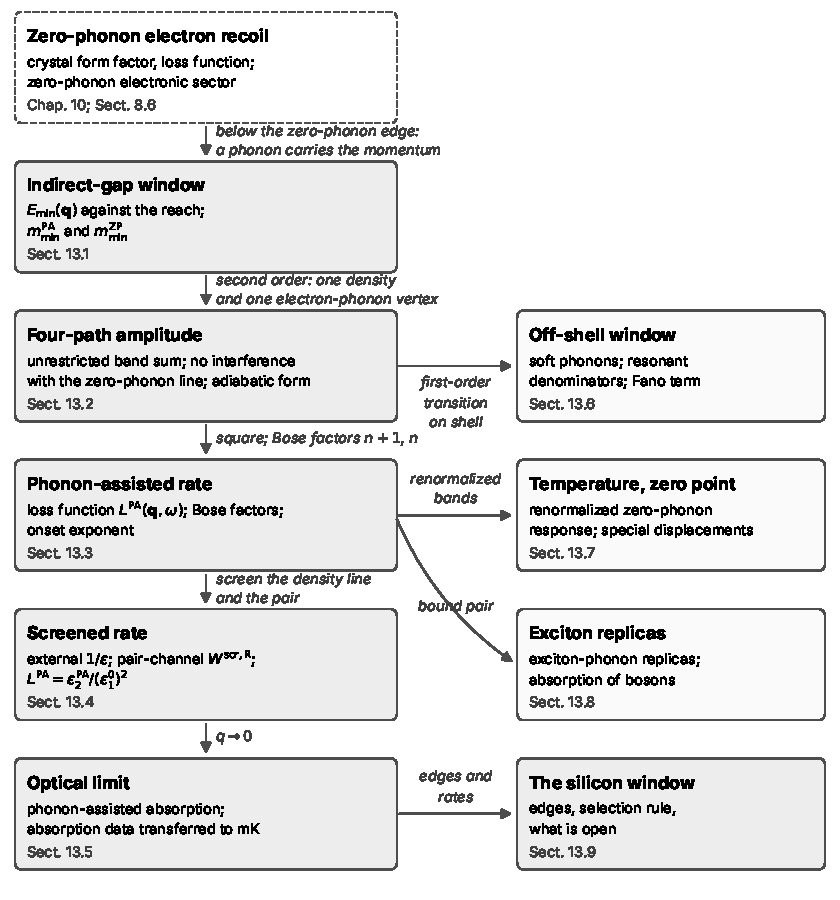
\includegraphics[width=0.85\linewidth]{figures/ch13/map13.pdf}
  \caption{Phonon-assisted electron recoil, from the kinematics of the window to the silicon window itself. Below the zero-phonon edge of the electronic response of \cref{chap:10}, a phonon must carry the missing crystal momentum (\cref{sec:13.1}). The amplitude is of second order, with one density vertex and one electron--phonon vertex on four paths (\cref{sec:13.2}); squared and summed over final states it gives the phonon-assisted loss function and rate (\cref{sec:13.3}), which screening dresses on the density line and on the pair (\cref{sec:13.4}); at $q \to 0$ it becomes phonon-assisted optical absorption (\cref{sec:13.5}; \cref{lim:13.5a}). The figure also places the off-shell window outside which the second-order rate is not separately defined (\cref{sec:13.6}), the renormalized bands at finite temperature and zero point (\cref{sec:13.7}; \cref{lim:13.7a}), and the bound pair with its phonon replicas and the absorption of bosonic dark matter (\cref{sec:13.8}). The edges and rates meet in the silicon window (\cref{sec:13.9}).}
  \label{fig:13-map}
\end{figure}

\section{The indirect-gap window}\label{sec:13.1}

A dark-matter particle of \SI{0.35}{MeV} can deposit up to $\frac12\mchi v_{\mathrm{max}}^2 = \SI{1.23}{eV}$, more than the \SI{1.17}{eV} gap of silicon, but only at the momentum transfer $q = \mchi v_{\mathrm{max}} = \SI{0.93}{keV}$. This momentum transfer is less than half of the \SI{1.94}{keV} that separates the valence-band maximum from the conduction valleys, and at $q = \SI{0.93}{keV}$ the cheapest electron--hole pair along the valley axis costs about \SI{1.9}{eV} (\cref{fig:3-si-bands}). Without a phonon the particle cannot create a pair. With a phonon of about \SI{15}{meV} that takes up the remaining \SI{1.0}{keV} of the valley momentum, it can. The phonon-assisted process of \cref{sec:9.1} is then the only way for dark matter scattering on electrons to create an electron--hole pair, in a window of masses that runs from the lightest mass that creates a pair with a phonon, $m_{\mathrm{min}}^{\mathrm{PA}}$, to the lightest mass that creates a pair without a phonon, $m_{\mathrm{min}}^{\mathrm{ZP}}$.

\subsection{The zero-phonon threshold mass}

The largest momentum transfer of a particle of mass $\mchi$ is $2\mchi v_{\mathrm{max}}$, and it reaches the valley momentum $k_{\mathrm{c}} = \SI{1.94}{keV}$ of \cref{eq:3.3-kc} only for $\mchi \ge k_{\mathrm{c}}/2v_{\mathrm{max}} = \SI{0.366}{MeV}$; at that mass the particle reaches $k_{\mathrm{c}}$ by backscattering, with no energy to spare. The energy that the particle can deposit at fixed $q$ is $qv_{\mathrm{max}} - q^2/2\mchi$ (\cref{eq:1.3-region}), largest at $q = \mchi v_{\mathrm{max}}$. The two requirements conflict: depositing the gap favors $q \approx \mchi v_{\mathrm{max}}$, while reaching the valley needs $q \approx k_{\mathrm{c}}$, and for light particles $\mchi v_{\mathrm{max}}$ is well below $k_{\mathrm{c}}$.

To locate the zero-phonon threshold, we turn the kinematic condition \cref{eq:3.3-allowed} into a condition on the mass. At fixed $\vect{q}$, a pair of energy $E$ is reachable when $qv_{\mathrm{max}} - q^2/2\mchi \ge E$. For $qv_{\mathrm{max}} > E$ this condition reads
\begin{equation*}
  \mchi \ge \frac{q^2}{2\,(qv_{\mathrm{max}} - E)} .
\end{equation*}
The right-hand side grows with $E$ at fixed $q$, so at each $\vect{q}$ the cheapest pair sets the bound, and the energy of that pair is the minimum pair energy $E_{\mathrm{min}}(\vect{q})$ of \cref{eq:3.3-Emin}. Minimizing then over $\vect{q}$, and writing out the minimum over the hole's crystal momentum $\vect{k}$ that $E_{\mathrm{min}}$ contains, gives the zero-phonon threshold mass
\begin{equation}
  m_{\mathrm{min}}^{\mathrm{ZP}} = \min_{\vect{q}}\frac{q^2}{2\,[qv_{\mathrm{max}} - E_{\mathrm{min}}(\vect{q})]}
  = \min_{\vect{q},\,\vect{k},\,v,\,c}\frac{q^2}{2\,[qv_{\mathrm{max}} - \varepsilon_{c,\vect{k}+\vect{q}} + \varepsilon_{v\vect{k}}]} ,
  \label{eq:13.1-mZP}
\end{equation}
with the minimum over the region where the denominator is positive. The second form is one minimization over six continuous variables, three for $\vect{q}$ and three for $\vect{k}$, and it shows that two common simplifications, fixing the hole at the valence-band maximum and restricting $\vect{q}$ to a few directions, can only raise the result.

Near a valley the minimization can be done by hand. Along the axis of a silicon valley, the pair energy is the parabola \cref{eq:3.3-Eminpar}, $E_{\mathrm{min}} \simeq \Eg + (q - k_{\mathrm{c}})^2/2M_{\mathrm{eh}}$, where $M_{\mathrm{eh}} = m^*_\parallel + m_{\mathrm{hh}}$ is the mass with which the pair as a whole recoils, equal to the sum of the longitudinal electron mass and the heavy-hole mass in the same direction. With $m^*_\parallel = 0.916\,m_e$ and $m_{\mathrm{hh}} = 0.277\,m_e$ along [100] (\cref{tab:3-materials}), $M_{\mathrm{eh}} = 1.19\,m_e$. Inserted in \cref{eq:13.1-mZP}, the parabola gives $m_{\mathrm{min}}^{\mathrm{ZP}} = \SI{0.425}{MeV}$ at $q = \SI{1.46}{keV}$. At that point the particle falls \SI{0.48}{keV} short of the valley, and the pair absorbs the shortfall as kinetic energy, $(\SI{0.48}{keV})^2/2M_{\mathrm{eh}} = \SI{0.19}{eV}$, for a total pair energy of \SI{1.36}{eV}. Lighter particles would have to transfer still less momentum, and the kinetic energy of the pair grows quadratically with the shortfall while the energy available grows only linearly with $\mchi$. The first-principles bands of \cref{fig:3-si-bands}, used along the same axis, give \SI{0.420}{MeV} at $q = \SI{1.43}{keV}$.

The pair need not move along the valley axis, and the hole need not sit at the valence-band maximum; the heavy-hole surfaces of silicon are strongly warped (\cref{eq:3.3-holes}), and a hole that moves into a flat direction lowers the kinetic energy of the pair. The full minimization \cref{eq:13.1-mZP} therefore gives a threshold mass below \SI{0.42}{MeV}, off the axis. \Cref{sec:13.9} gives its value and explains why the first zero-phonon states reached at that threshold are weakly coupled. Binding the pair into an exciton changes the threshold mass only slightly. The $1s$ exciton lies $E_x^b = \SI{14.7}{meV}$ below the free pair (\cref{sec:4.9}). Since $\partial\mchi/\partial E = \mchi/(qv_{\mathrm{max}} - E)$ at fixed $q$, the exciton lowers the threshold mass by $\mchi E_x^b/(qv_{\mathrm{max}} - E) = \SI{0.0025}{MeV}$ at the parabolic optimum, about \SI{0.6}{\percent}.

\subsection{The phonon-assisted onset}

A phonon changes the bookkeeping of crystal momentum. The dark matter transfers $\vect{q}$; the electron ends at $\vect{k}_e$ in a conduction band, the hole at $\vect{k}_h$ in a valence band, and a phonon of branch $\nu$ and wavevector $\vect{Q}$ is emitted. Conservation of crystal momentum fixes $\vect{Q} = \vect{k}_e - \vect{k}_h - \vect{q}$ up to a reciprocal-lattice vector, and the energy deposited is $\varepsilon_{c\vect{k}_e} - \varepsilon_{v\vect{k}_h} + \omega_{\vect{Q}\nu}$. The phonon takes whatever crystal momentum the pair needs, and since no phonon of silicon has more than \SI{64}{meV} (\cref{sec:5.2}), that momentum costs at most a few percent of the gap. The cheapest final state puts the electron at the bottom of a valley and the hole at the valence-band maximum. At momentum transfer $\vect{q}$ it costs
\begin{equation}
  E_{\mathrm{min}}^{\mathrm{PA}}(\vect{q}) = \Eg + \min_\nu\,\omega_{\vect{k}_{\mathrm{c}} - \vect{q},\,\nu} ,
  \label{eq:13.1-EPA}
\end{equation}
with $\vect{k}_{\mathrm{c}}$ the valley that makes the phonon cheapest, chosen among the six valleys and their images under reciprocal-lattice vectors. Compared to the zero-phonon edge, the phonon-assisted threshold hardly depends on $\vect{q}$. It falls to $\Eg$ only at $\vect{q} = \vect{k}_{\mathrm{c}}$, where the acoustic phonon needed has zero energy, and it never rises above $\Eg + \SI{64}{meV}$. Moving the electron and the hole off the band extrema could lower the phonon energy but adds kinetic energy to the pair. With the dispersion of \cref{sec:5.2}, the best trade between phonon energy and kinetic energy lowers the threshold by less than \SI{0.02}{meV}, an amount we neglect.

\Cref{eq:13.1-EPA} assumes that the phonon is emitted. At temperature $T$ the pair can also be created by absorbing a phonon. Absorption costs $\Eg - \omega_{\vect{Q}\nu}$ but comes with the occupation $n_{\mathrm{B}}(\omega_{\vect{Q}\nu})$ in place of $n_{\mathrm{B}} + 1$ (\cref{sec:5.3}), and $\Eg$ itself shifts with $T$ (\cref{sec:13.7}). For the transverse acoustic phonon of about \SI{15}{meV} that sets the onset below, $n_{\mathrm{B}}$ is 0.12 at \SI{77}{K}, $2\times10^{-19}$ at \SI{4}{K} and $3\times10^{-75}$ at \SI{1}{K}. The absorption sideband, which would open at \SI{0.329}{MeV}, is absent in a detector at millikelvin temperatures. At those temperatures only emission counts, and $\Eg$ is the gap extrapolated to zero temperature.

The onset mass follows from \cref{eq:13.1-EPA} as $m_{\mathrm{min}}^{\mathrm{ZP}}$ followed from $E_{\mathrm{min}}$:
\begin{equation}
  m_{\mathrm{min}}^{\mathrm{PA}} = \min_{\vect{q}}\frac{q^2}{2\,[qv_{\mathrm{max}} - E_{\mathrm{min}}^{\mathrm{PA}}(\vect{q})]} .
  \label{eq:13.1-mPAdef}
\end{equation}
For a threshold $E$ independent of $q$, the minimum sits at $q = 2E/v_{\mathrm{max}}$ and equals the floor $2E/v_{\mathrm{max}}^2$ of \cref{eq:1.3-mmin}. Here $E$ varies with $q$, but slowly. Write $E(q)$ for $E_{\mathrm{min}}^{\mathrm{PA}}$ along a line of $\vect{q}$ and $E' = \dd E/\dd q$. Setting the derivative of $q^2/[2(qv_{\mathrm{max}} - E)]$ to zero gives $qv_{\mathrm{max}} - 2E + qE' = 0$. The optimum is therefore $q^* = 2E/(v_{\mathrm{max}} + E')$, and inserting $q^*$ back into \cref{eq:13.1-mPAdef} gives
\begin{equation}
  m_{\mathrm{min}}^{\mathrm{PA}} = \frac{2\,[\Eg + \omega_\nu(\vect{Q}^*)]}{v_{\mathrm{max}}^2 - u_\nu^2} ,
  \qquad \vect{Q}^* = \vect{k}_{\mathrm{c}} - \vect{q}^* ,\quad q^* \simeq \frac{2\,[\Eg + \omega_\nu(\vect{Q}^*)]}{v_{\mathrm{max}}} ,
  \label{eq:13.1-mPA}
\end{equation}
where $u_\nu = |E'|$ is the group velocity of the phonon along $\vect{q}$ at $\vect{Q}^*$ and the branch $\nu$ is the one that gives the smallest result. The slope of the dispersion enters only squared, because $q^*$ is a stationary point: moving $q$ slightly changes the phonon energy to first order but the mass only to second. Phonon group velocities are a few km/s, below the speeds of sound, against $v_{\mathrm{max}} = \SI{794.5}{km.s^{-1}}$, and $u_\nu^2/v_{\mathrm{max}}^2 \sim 10^{-5}$. To that accuracy the onset is the kinematic floor with the gap raised by the energy of one phonon, at the wavevector $\vect{Q}^*$ that the dark matter leaves for the phonon. \Cref{eq:13.1-mPA} is implicit, since $\vect{Q}^*$ depends on $q^*$, but one or two iterations starting from $\omega = 0$ settle the value of $q^*$.

\begin{keyresult}[Window kinematics]
In an indirect-gap crystal at zero temperature, scattering dark matter creates an electron--hole pair only above the phonon-assisted onset $m_{\mathrm{min}}^{\mathrm{PA}}$ of \cref{eq:13.1-mPA}, and without a phonon only above the zero-phonon threshold $m_{\mathrm{min}}^{\mathrm{ZP}}$ of \cref{eq:13.1-mZP}. For
\begin{equation*}
  m_{\mathrm{min}}^{\mathrm{PA}} \le \mchi < m_{\mathrm{min}}^{\mathrm{ZP}} ,
\end{equation*}
the phonon-assisted process is the only electron-recoil channel. Bound pairs lower both edges of the window by replacing $\Eg$ with $\Eg - E_x^b$ in the corresponding threshold.
\end{keyresult}

The onset is set by the branch of lowest energy at $\vect{Q}^*$, whatever its coupling strength. In silicon the transverse acoustic (TA) branch is the lowest everywhere away from the zone center, and \cref{we:13-onset} finds $\omega_{\mathrm{TA}}(\vect{Q}^*) = \SI{14.8}{meV}$ at $|\vect{Q}^*| = 0.46\,(2\pi/a)$, with $\vect{q}^*$ along the valley axis. Tilting $\vect{q}$ away from the axis raises the TA energy at $\vect{Q}^*$, by \SI{0.7}{meV} at a tilt of \SI{0.3}{rad} in a $\{001\}$ plane, so the onset is on the axis. The longitudinal acoustic and transverse optical branches open later, at 0.341 and \SI{0.350}{MeV}. Compared to light, dark matter needs a phonon of shorter wavevector and lower energy. A photon carries no momentum on the scale of the zone, so in optical absorption the phonon must supply all of $\vect{k}_{\mathrm{c}}$, and the TA phonon that sets the optical edge has \SI{18.27}{meV}~\cite{macfarlane1958fine} (\cref{sec:6.5}). A particle at the onset supplies $q^* = \SI{0.90}{keV}$ itself, about half of $k_{\mathrm{c}}$, and leaves the phonon a shorter wavevector on the flat part of the TA branch.

\Cref{fig:13-window} puts the two thresholds side by side. In panel (a) the zero-phonon edge $E_{\mathrm{min}}(\vect{q})$ dips to $\Eg$ only near $k_{\mathrm{c}}$, while the phonon-assisted threshold \cref{eq:13.1-EPA} runs almost flat just above $\Eg$ at every $q$. The parabola of a \SI{0.3}{MeV} particle stays below both thresholds. The parabola of a \SI{0.4}{MeV} particle crosses the phonon-assisted threshold but not, along these directions, the zero-phonon edge; a \SI{0.5}{MeV} particle reaches both thresholds. Panel (b) shows the same comparison as two curves of threshold mass against $q$, and the minima of the two curves are \cref{eq:13.1-mZP,eq:13.1-mPAdef}: the phonon-assisted curve has a broad minimum near \SI{0.9}{keV}, the zero-phonon curve a narrow one near \SI{1.4}{keV}.

\begin{figure}[tbp]
  \centering
  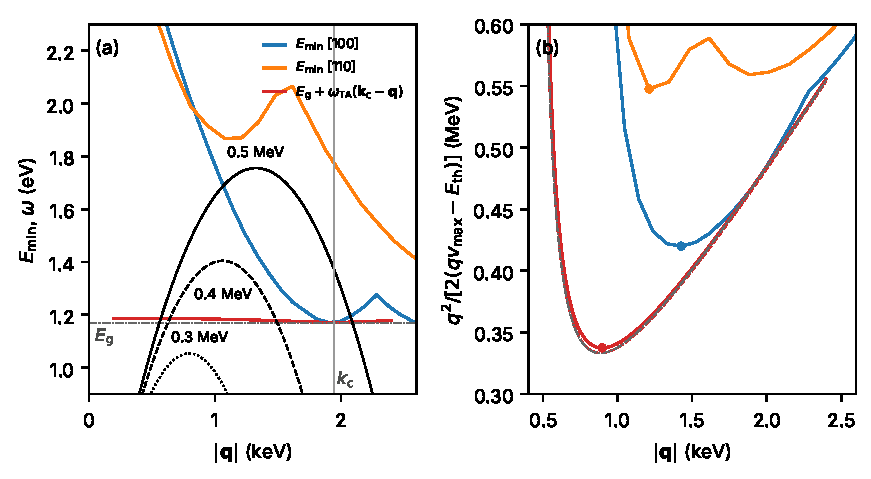
\includegraphics[width=\linewidth]{figures/ch13/fig13_1.pdf}
  \caption{Kinematics of the indirect-gap window of silicon. (a)~Minimum pair energy $E_{\mathrm{min}}(\vect{q})$ (\cref{eq:3.3-Emin}) for $\vect{q}$ along [100] and [110], and the phonon-assisted threshold $\Eg + \omega_{\mathrm{TA}}(\vect{k}_{\mathrm{c}} - \vect{q})$ (\cref{eq:13.1-EPA}) for $\vect{q}$ along [100], with the electron at the valley minimum $\vect{k}_{\mathrm{c}} = 0.85\,(2\pi/a)(1,0,0)$ and the hole at the valence-band maximum. Black: the largest energy deposited, $qv_{\mathrm{max}} - q^2/2\mchi$, for $\mchi = 0.3$ (dotted), 0.4 (dashed) and \SI{0.5}{MeV} (solid), with $v_{\mathrm{max}} = 2.650\times10^{-3}$. Dash-dotted: $\Eg = \SI{1.17}{eV}$. (b)~The lightest mass that reaches each threshold at momentum transfer $q$, $q^2/[2(qv_{\mathrm{max}} - E_{\mathrm{th}})]$; dots mark the minima over $q$. Red solid: phonon-assisted, free pair, minimum \SI{0.3374}{MeV} at $q = \SI{0.90}{keV}$; red dashed: bound pair, $\Eg$ lowered by $E_x^b = \SI{14.7}{meV}$, minimum \SI{0.3332}{MeV}; grey dash-dotted: the floor $2\Eg/v_{\mathrm{max}}^2$ at fixed threshold $\Eg$. Blue and orange: zero-phonon, with minima \SI{0.420}{MeV} along [100] and \SI{0.548}{MeV} along [110]; these are upper values for the zero-phonon threshold, since the joint minimum over all directions of $\vect{q}$ and all hole momenta lies lower. The [111] direction, whose $E_{\mathrm{min}}$ stays above \SI{2.13}{eV}, is off scale (minimum \SI{0.615}{MeV}). Bands: PBE calculation of \cref{fig:3-si-bands} at $a = \SI{5.431}{\angstrom}$ on a grid of $48^3$ crystal momenta, without spin--orbit coupling, with the conduction bands shifted up by \SI{0.613}{eV} so that the indirect gap equals the measured \SI{1.17}{eV}. Phonons: PBE force constants of \cref{sec:5.2} at the same lattice constant. The TA branch of these force constants is \SI{8}{\percent} below the neutron data at X, and scaling it up to the data raises the phonon-assisted minimum to \SI{0.3378}{MeV}.}
  \label{fig:13-window}
\end{figure}

\begin{workedexample}{The phonon-assisted onset of silicon}\label{we:13-onset}
We evaluate \cref{eq:13.1-mPA} with the measured gap extrapolated to zero temperature, $\Eg = \SI{1.17}{eV}$, the valley at $k_{\mathrm{c}} = 0.85\,(2\pi/a) = \SI{1940}{eV}$ (\cref{we:3-kc}), $v_{\mathrm{max}}^2 = 7.023\times10^{-6}$, and the TA branch of the force constants of \cref{sec:5.2}, with $\vect{q}$ along the valley axis.

\emph{First pass, no phonon energy.} $q^* = 2\Eg/v_{\mathrm{max}} = \SI{883}{eV}$, which leaves the phonon $Q^* = k_{\mathrm{c}} - q^* = \SI{1057}{eV} = 0.463\,(2\pi/a)$. The TA energy there is \SI{14.87}{meV}.

\emph{Second pass.} With $E = \Eg + \omega_{\mathrm{TA}}(\vect{Q}^*) = \SI{1.1849}{eV}$, $q^* = 2E/v_{\mathrm{max}} = \SI{894}{eV}$ and $Q^* = 0.458\,(2\pi/a) = \SI{0.53}{\angstrom^{-1}}$, where $\omega_{\mathrm{TA}}(\vect{Q}^*) = \SI{14.79}{meV}$. A third pass changes nothing at this precision. The slope of the TA branch at $Q^*$ is $u_{\mathrm{TA}} = \SI{2.1}{km.s^{-1}}$, and $u_{\mathrm{TA}}^2/v_{\mathrm{max}}^2 = 7\times10^{-6}$ is negligible. The onset is
\begin{equation*}
  m_{\mathrm{min}}^{\mathrm{PA}} = \frac{2\times(\SI{1.17}{eV} + \SI{0.01479}{eV})}{7.023\times10^{-6}} = \SI{0.3374}{MeV} ,
\end{equation*}
\SI{1.3}{\percent} above the floor $2\Eg/v_{\mathrm{max}}^2 = \SI{0.3332}{MeV}$. The direct minimization of \cref{eq:13.1-mPAdef} on a grid of $q$ gives the same value, at $q = \SI{0.90}{keV}$.

\emph{Sensitivity.} An error $\delta\omega$ in the phonon energy moves the onset by $2\,\delta\omega/v_{\mathrm{max}}^2 = \SI{2.8e-4}{MeV}$ per meV. The TA branch of this calculation is \SI{8}{\percent} soft at X; scaling the whole branch up to the neutron value there gives $\omega_{\mathrm{TA}}(\vect{Q}^*) = \SI{16.1}{meV}$ and an onset of \SI{0.3378}{MeV}. Had the phonon to supply all of $\vect{k}_{\mathrm{c}}$, as for light, the \SI{18.27}{meV} of the optical edge would put the onset at \SI{0.3384}{MeV}.

\emph{Bound pair.} The $1s$ exciton replaces $\Eg$ by $\Eg - E_x^b = \SI{1.1553}{eV}$. The same passes give $q^* = 2E/v_{\mathrm{max}} = \SI{0.883}{keV}$, where $\omega_{\mathrm{TA}}(\vect{Q}^*) = \SI{14.87}{meV}$, and the onset becomes $2\times\SI{1.1702}{eV}/v_{\mathrm{max}}^2 = \SI{0.3332}{MeV}$; the direct minimization puts the optimum at \SI{0.885}{keV} with the same onset. The phonon energy and the binding energy nearly cancel, and the bound-pair onset falls on the floor $2\Eg/v_{\mathrm{max}}^2$ that a crystal with a direct gap of \SI{1.17}{eV} would have. The strength of this phonon replica of the $1s$ exciton, compared with the free-pair continuum above it, is a question for \cref{sec:13.8}.
\end{workedexample}

\subsection{Germanium and a direct-gap crystal}

Germanium has its valleys at the L points, at $|\vect{k}_{\mathrm{c}}| = |\mathrm{\Gamma}\mathrm{L}| = \SI{1.90}{keV}$, almost the momentum of the silicon valleys, but a gap of only \SI{0.744}{eV} (\cref{sec:3.3}). Its floor $2\Eg/v_{\mathrm{max}}^2$ is \SI{0.212}{MeV}, at $q = \SI{0.56}{keV}$, and the phonon must supply the remaining \SI{1.34}{keV}, about 0.7 of the way from $\mathrm{\Gamma}$ to L. Along that line the transverse acoustic branch of germanium rises monotonically to \SI{1.9}{THz}, \SI{7.9}{meV}, at L~\cites{nilsson1971phonon}[Table~IV]{haxhijaj2026lattice}, so $\omega_{\mathrm{TA}}(\vect{Q}^*) \le \SI{7.9}{meV}$, and \cref{eq:13.1-mPA} places the phonon-assisted onset between 0.2119 and \SI{0.2141}{MeV}. The bracket needs no band structure and no computed phonon, only the gap, the position of L and the measured TA branch.

The zero-phonon threshold of germanium is harder to pin down. \Cref{we:3-mmin} bracketed it between 0.212 and \SI{0.420}{MeV}. On the L axis, with the parabola of \cref{eq:3.3-Eminpar} and $M_{\mathrm{eh}} = m^*_\parallel + m_{\mathrm{hh}} = (1.59 + 0.469)\,m_e = 2.06\,m_e$ along [111] (\cref{tab:3-materials}), \cref{eq:13.1-mZP} gives \SI{0.32}{MeV} at $q = \SI{1.10}{keV}$. The heavy longitudinal mass of the L valleys makes the kinetic energy of the momentum shortfall small, and the zero-phonon edge sits much closer to the onset, in relative terms, than in silicon. The value of \SI{0.32}{MeV} is a guide, not a bound on the zero-phonon edge: the minimum need not lie on the axis, and the heavy hole of germanium is warped and strongly mixed by spin--orbit coupling ($\Delta_{\mathrm{SO}} = \SI{0.296}{eV}$). \Cref{sec:13.9-ge-gaas} states what is known of the edge.

The route through the direct gap at $\mathrm{\Gamma}$ plays no part: as \cref{we:3-mmin} showed, the light pair at the direct gap opens only at a few MeV.

A direct-gap crystal has a window as well. Take GaAs, with both band edges at $\mathrm{\Gamma}$ and a gap of \SI{1.52}{eV}. Its floor is $2\Eg/v_{\mathrm{max}}^2 = \SI{0.433}{MeV}$, and below that mass dark matter scattering creates no pair in GaAs, with or without a phonon. At the masses of the silicon and germanium windows a direct-gap crystal of this gap has no electron-recoil channel. Above the floor, however, energy and momentum conflict again. A pair at rest at $\mathrm{\Gamma}$ costs exactly $\Eg$, but the particle deposits $\Eg$ only near $q^* = 2\Eg/v_{\mathrm{max}} = \SI{1.15}{keV}$, and a zero-phonon pair that carries this momentum has kinetic energy $q^{*2}/2M_{\mathrm{eh}}$. The electron of GaAs is light, $0.067\,m_e$, and with a heavy hole along [100] or [111] the pair mass is $M_{\mathrm{eh}} = 0.42$ or $0.96\,m_e$, and the kinetic energy is 3.1 or \SI{1.3}{eV}, comparable to the gap itself. For a pair of mass $M_{\mathrm{eh}}$ at $\mathrm{\Gamma}$, the condition for the pair to be reachable is $qv_{\mathrm{max}} - q^2/2\mchi - q^2/2M_{\mathrm{eh}} \ge \Eg$. Its left-hand side is largest at $q = \mu v_{\mathrm{max}}$, with $\mu = \mchi M_{\mathrm{eh}}/(\mchi + M_{\mathrm{eh}})$, where it equals $\frac12\mu v_{\mathrm{max}}^2$. Writing $m_{\mathrm{g}} = 2\Eg/v_{\mathrm{max}}^2$ for the floor, the zero-phonon threshold of a direct gap is therefore
\begin{equation}
  m_{\mathrm{min}}^{\mathrm{ZP}} = \frac{m_{\mathrm{g}}M_{\mathrm{eh}}}{M_{\mathrm{eh}} - m_{\mathrm{g}}} \qquad (M_{\mathrm{eh}} > m_{\mathrm{g}}) ,
  \label{eq:13.1-mZPdir}
\end{equation}
and there is none when $M_{\mathrm{eh}} \le m_{\mathrm{g}}$. For GaAs, $m_{\mathrm{g}} = 0.847\,m_e$: in the parabolic approximation, the pair with the [100] heavy hole never opens, and the pair with the [111] heavy hole opens at \SI{3.7}{MeV}. A phonon supplies the momentum, as in silicon: it carries $\vect{Q} \approx -\vect{q}^*$, about half the way to the zone boundary, and leaves the pair at rest. The transverse acoustic branch is the cheapest, and it stays below the \SI{10.5}{meV} that the computed dispersion gives at X (\cref{tab:5-phonons}). The computed \SI{10.5}{meV} is an upper value, since the computed branch lies above the measured one at X, and \cref{eq:13.1-mPA} gives an onset of 0.433 to \SI{0.436}{MeV}. The first zero-phonon states that a particle near this mass can reach are the states of the L valleys, which lie \SI{1.815}{eV} above the valence-band maximum, at $|\mathrm{\Gamma}\mathrm{L}| = \SI{1.90}{keV}$ (\cref{sec:3.3}). Their floor is $2\times\SI{1.815}{eV}/v_{\mathrm{max}}^2 = \SI{0.517}{MeV}$, and depositing \SI{1.815}{eV} at exactly $|\mathrm{\Gamma}\mathrm{L}|$ needs \SI{0.560}{MeV}, so the zero-phonon edge of the L valleys lies between 0.517 and \SI{0.560}{MeV}. GaAs therefore has a phonon-assisted window too, from \SI{0.43}{MeV} to above \SI{0.5}{MeV}, but it begins above the masses at which the silicon window has already closed.

A window thus exists in any crystal whose pairs cannot absorb the momentum $q^* \approx 2\Eg/v_{\mathrm{max}}$ for less than a phonon energy, that is, whenever $|\vect{q}^* - \vect{k}_{\mathrm{c}}|^2/2M_{\mathrm{eh}}$ exceeds the phonon energies at the corresponding $\vect{Q}^*$. For band masses of order $m_e$ and $q^* \sim \SI{1}{keV}$ the kinetic energy of the pair is of order an eV, a hundred times a phonon energy, and the condition is met in silicon, germanium and GaAs alike. In silicon and germanium the indirect gap places the windows low. The two windows start at the floors of their crystals, 0.333 and \SI{0.212}{MeV}, where no direct-gap crystal of comparable gap has any electron recoil. The optical absorption edges of silicon and germanium are phonon-assisted, and they measure the same kind of amplitude in the limit $q \to 0$ (\cref{sec:13.5}).

\section{The phonon-assisted amplitude}\label{sec:13.2}

At the onset of \cref{we:13-onset} a particle of \SI{0.3374}{MeV} transfers $q^* = \SI{0.90}{keV}$ along a valley axis of silicon and deposits \SI{1.185}{eV}. The final state has a hole at the valence-band maximum, an electron at the bottom of a conduction valley, \SI{1.94}{keV} away in crystal momentum, and a transverse acoustic phonon of \SI{14.8}{meV} that carries the remaining \SI{1.0}{keV}. Neither the density coupling nor the electron--phonon coupling reaches this final state alone. The density $n_e(\vect{q})$ creates pairs of crystal momentum $\vect{q}$, and at $q = \SI{0.90}{keV}$ the cheapest of them costs about \SI{1.9}{eV} (\cref{fig:13-window}). The electron--phonon coupling creates a phonon and can change the crystal momentum of an electron by any amount, but it cannot lift an electron across a gap of \SI{1.17}{eV} with the tens of meV that a phonon brings. The amplitude is therefore of second order, with one density vertex and one electron--phonon vertex.

\subsection{Final states and the second-order amplitude}

The target is the crystal at the base point of \cref{sec:8.5} with one coupling added: independent electrons in Bloch states $\psi_{n\vect{k}}$ with energies $\varepsilon_{n\vect{k}}$ (Kohn--Sham energies with the conduction bands raised by the scissor shift, as in \cref{sec:10.1}), harmonic phonons $(\vect{Q},\nu)$ with energies $\omega_{\vect{Q}\nu}$, and the electron--phonon Hamiltonian $H_{\mathrm{ep}}$ of \cref{eq:A.6-Hep}, linear in the displacements, with the screened vertex $g_{mn\nu}(\vect{k},\vect{Q})$ of \cref{eq:A.6-g}. The dark matter couples to the electron density, through the row of \cref{eq:8.2-spectrum} with $\mathfrak{D}_{ee} = |\tilde V(\vect{q})|^2$. The target enters only through the matrix elements of $n_e(\vect{q})$ (\cref{eq:3.2-ne}) that appear in the structure factor \cref{eq:4.2-Sab}. In the zero-phonon response of \cref{sec:10.1}, the matrix element of $n_e(\vect{q})$ is the density vertex $\rho_{cv}(\vect{k},\vect{q})$ of \cref{eq:3.2-rho}. In the phonon-assisted response a second-order amplitude replaces the density vertex.

The initial state $|i\rangle$ has the valence bands filled, the conduction bands empty and $n_{\vect{Q}\nu}$ phonons in each mode. A one-phonon final state has an electron in $(c,\vect{k}')$, a hole in $(v,\vect{k})$ and the phonon occupations of $|i\rangle$ changed in one mode,
\begin{equation}
  |f\rangle = c^\dagger_{c\vect{k}'}c_{v\vect{k}}\,|i'\rangle , \qquad
  \vect{k}' = \vect{k} + \vect{q} + \vect{Q} , \qquad
  E_f - E_i = \varepsilon_{c\vect{k}'} - \varepsilon_{v\vect{k}} \pm \omega_{\vect{Q}\nu} ,
  \label{eq:13.2-final}
\end{equation}
where $|i'\rangle$ has one phonon more in $(-\vect{Q},\nu)$ (upper sign, emission) or one fewer in $(\vect{Q},\nu)$ (lower sign, absorption), as in \cref{eq:A.6-weights}, and $\vect{k}'$ is folded back into the zone. The momentum transfer $\vect{q}$ is not folded: the density vertex keeps it whole and carries the Umklapp vector in its plane wave (\cref{eq:3.2-rho}). Conservation of crystal momentum leaves the phonon whatever crystal momentum the pair needs beyond $\vect{q}$: $\vect{Q} = \vect{k}' - \vect{k} - \vect{q}$ modulo a reciprocal-lattice vector, as in \cref{sec:13.1}. The density vertex and the electron--phonon vertex are both diagonal in spin, so the electron and the hole have the same spin, and the spin sum enters only the rate (\cref{sec:13.3}). With spin--orbit coupling the bands are spinors, and the formulas below hold with the band indices running over spinor bands.

The second-order amplitude follows from \cref{eq:2.4-c2} as for light (\cref{sec:6.5}). The dark matter gives up the energy $\omega$ and the momentum $\vect{q}$ at its own vertex, and its kinetic energy cancels from every denominator. In the ordering in which the density vertex acts first, the intermediate state $|m\rangle$ already holds the energy $\omega$; in the ordering in which the electron--phonon vertex acts first, the intermediate state does not:
\begin{equation}
  \langle f|n_e^{(2)}(\vect{q})|i\rangle = \sum_m\left[\frac{\langle f|H_{\mathrm{ep}}|m\rangle\langle m|n_e(\vect{q})|i\rangle}{E_i + \omega - E_m} + \frac{\langle f|n_e(\vect{q})|m\rangle\langle m|H_{\mathrm{ep}}|i\rangle}{E_i - E_m}\right] , \qquad
  \omega = E_f - E_i .
  \label{eq:13.2-T}
\end{equation}
This matrix element takes the place of $\langle f|n_e(\vect{q})|i\rangle$ in \cref{eq:4.2-Sab}. The condition $\omega = E_f - E_i$ is the energy delta function of the structure factor, and the amplitude is needed only there, on the energy shell. The sum runs over many-electron states with their phonons, and it is finite as long as no $E_m$ equals $E_i + \omega$ or $E_i$. An $E_m$ equal to $E_i$ never occurs in an insulator. An $E_m$ equal to $E_i + \omega$ would mean that the density alone creates a real zero-phonon pair at $(\vect{q},\omega)$, and no such pair exists while $\omega$ lies below $E_{\mathrm{min}}(\vect{q})$ (\cref{eq:13.2-doff}).

\subsection{Four paths}

Both vertices are one-body operators, $n_e(\vect{q}) = \sum\rho_{mn}c^\dagger c$ and $H_{\mathrm{ep}} = N^{-1/2}\sum g_{mn\nu}c^\dagger c\,B_{\vect{Q}\nu}$, and each moves one electron. Acting first on the filled valence bands, a vertex can only move an electron from a filled state into an empty one, so every intermediate state $|m\rangle$ holds exactly one electron--hole pair. (A term that moves an electron back into the state it came from needs a momentum transfer equal to a reciprocal-lattice vector, $\vect{q} = \vect{G}$ or $\vect{Q} = 0$. It has measure zero in the integrals over $\vect{q}$ and $\vect{Q}$, and \cref{app:D.35} shows that even there it adds nothing new.) The second vertex must turn that intermediate pair into the final pair $(c\vect{k}';\,v\vect{k})$, again by moving one electron. The second vertex can do so in two ways. It can move the intermediate electron into $(c,\vect{k}')$, if the intermediate hole is already the final one, $(v,\vect{k})$; or it can move the electron of $(v,\vect{k})$ into the intermediate hole, if the intermediate electron is already the final one, $(c,\vect{k}')$. The two ways, combined with the two orderings of the vertices, make four paths:
\begin{equation}
  \begin{aligned}
  \text{A:}&\quad \frac{g_{cp\nu}(\vect{k}+\vect{q},\vect{Q})\,\rho_{pv}(\vect{k},\vect{q})}{\omega - \varepsilon_{p,\vect{k}+\vect{q}} + \varepsilon_{v\vect{k}}} ,
  &\text{B:}&\quad \frac{\rho_{cp}(\vect{k}+\vect{Q},\vect{q})\,g_{pv\nu}(\vect{k},\vect{Q})}{\varepsilon_{v\vect{k}} - \varepsilon_{p,\vect{k}+\vect{Q}} \mp \omega_{\vect{Q}\nu}} , &&\quad p\ \text{empty}, \\
  \text{C:}&\quad -\frac{\rho_{cp}(\vect{k}+\vect{Q},\vect{q})\,g_{pv\nu}(\vect{k},\vect{Q})}{\omega - \varepsilon_{c\vect{k}'} + \varepsilon_{p,\vect{k}+\vect{Q}}} ,
  &\text{D:}&\quad -\frac{g_{cp\nu}(\vect{k}+\vect{q},\vect{Q})\,\rho_{pv}(\vect{k},\vect{q})}{\varepsilon_{p,\vect{k}+\vect{q}} - \varepsilon_{c\vect{k}'} \mp \omega_{\vect{Q}\nu}} , &&\quad p\ \text{filled}.
  \end{aligned}
  \label{eq:13.2-paths}
\end{equation}
Each term is the contribution of one intermediate band $p$, with the common factor $N^{-1/2}(n_{\vect{Q}\nu} + \frac12 \pm \frac12)^{1/2}$ of the phonon vertex taken out. \Cref{fig:13-paths} draws the four paths as time-ordered diagrams.

\begin{figure}[tbp]
  \centering
  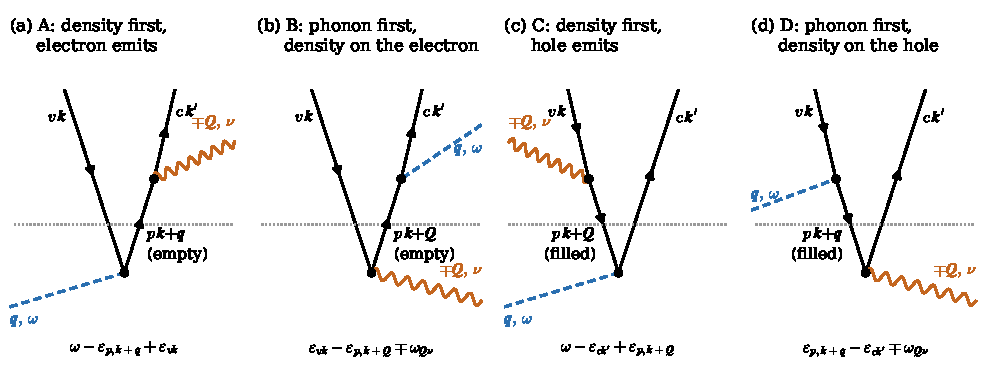
\includegraphics[width=\linewidth]{figures/ch13/fig13_2.pdf}
  \caption{The four paths of the phonon-assisted electron-recoil amplitude, \cref{eq:13.2-paths}, as time-ordered diagrams. Time runs upward. Lines with upward arrows are electrons, lines with downward arrows are holes; the dashed line is the dark-matter density vertex, which delivers momentum $\vect{q}$ and energy $\omega$; the wavy line is the phonon, emitted with $-\vect{Q}$ or absorbed with $+\vect{Q}$. The dotted line cuts the intermediate state, whose energy denominator is printed below each panel. Every path ends in the same final state, an electron in $(c,\vect{k}')$ with $\vect{k}' = \vect{k} + \vect{q} + \vect{Q}$ and a hole in $(v,\vect{k})$. (a)--(d)~Paths A to D, with an electron in an empty band $p$ between the vertices in A and B and a hole in a filled band $p$ in C and D. Schematic; no line length or angle carries a number.}
  \label{fig:13-paths}
\end{figure}

In paths A and B an electron propagates between the vertices. In A the density creates a pair, $(p,\vect{k}+\vect{q})$ with $(v,\vect{k})$, and the electron then scatters into $(c,\vect{k}')$ by emitting or absorbing the phonon; the pair created in A is the virtual zero-phonon pair of \cref{sec:10.1}, carried to the final state by the phonon. In B the phonon vertex creates a virtual pair at crystal momentum $\vect{Q}$, $(p,\vect{k}+\vect{Q})$ with $(v,\vect{k})$, and the density then scatters the electron by $\vect{q}$. The intermediate band $p$ must be empty in both A and B, since an electron cannot enter a filled state. In paths C and D a hole propagates. In C the density creates the final electron from a filled state $(p,\vect{k}+\vect{Q})$, and the phonon vertex then moves an electron from $(v,\vect{k})$ into the hole that the final electron left. In D the phonon vertex creates the final electron from a filled state $(p,\vect{k}+\vect{q})$, and the density then fills the hole in $(p,\vect{k}+\vect{q})$ from $(v,\vect{k})$. The denominators contain the energies of the intermediate pairs. They also contain $\omega$ in the density-first orderings A and C, and the phonon energy in the phonon-first orderings B and D, where the phonon has already been emitted or absorbed.

The minus signs of C and D come from the order of the fermion operators. In path A the operators act as $c^\dagger_cc_p\,c^\dagger_pc_v = c^\dagger_c(1 - n_p)c_v$, which is $c^\dagger_cc_v$ on a state with $p$ empty. In path C they act as $c^\dagger_pc_v\,c^\dagger_cc_p$, and three exchanges of neighboring operators bring them into the order $-c^\dagger_c\,(c^\dagger_pc_p)\,c_v = -c^\dagger_c\,n_p\,c_v$, which is $-c^\dagger_cc_v$ on a state with $p$ filled. The same reordering gives $-1$ for D. The four paths are those of phonon-assisted absorption (\cref{sec:6.5}), with the velocity vertex of light replaced by the density vertex; summed over every band they give the two-term amplitude of phonon-assisted absorption~\cites[Eq.~(200)]{giustino2017electron}[Eqs.~(2) and~(3)]{noffsinger2012phonon}. Replacing the velocity vertex by the density vertex changes the crystal momenta at which the intermediate states sit: the photon-first intermediate state of \cref{eq:6.5-M} sits at the crystal momentum of the hole, and the density-first intermediate state of path A at $\vect{k}+\vect{q}$.

\subsection{The unrestricted band sum}

On the energy shell the hole paths change form. Insert $\omega = \varepsilon_{c\vect{k}'} - \varepsilon_{v\vect{k}} \pm \omega_{\vect{Q}\nu}$ of \cref{eq:13.2-final} into their denominators. The denominator of C becomes $\varepsilon_{p,\vect{k}+\vect{Q}} - \varepsilon_{v\vect{k}} \pm \omega_{\vect{Q}\nu}$, and with its minus sign, path C becomes the expression of path B for a filled band $p$. The denominator of D becomes $\varepsilon_{p,\vect{k}+\vect{q}} - \varepsilon_{v\vect{k}} - \omega$, and path D becomes the expression of path A for a filled band. A single electron could not take paths A and B through a filled band: Pauli blocking forbids them. In the many-electron amplitude the blocked paths return as exchange partners, paths C and D, with exactly the one-electron value. In path C the electron that ends in $(c,\vect{k}')$ comes from the filled band $p$, and the electron from $(v,\vect{k})$ takes its place; exchanging the two identical electrons turns path C into path B with the electron from $v$ passing through $p$. The fermion sign of the exchange and the sign of the hole denominator cancel, and the four paths combine into the amplitude of one electron alone in the bands:
\begin{keyresult}[Phonon-assisted amplitude]
On the energy shell, the second-order amplitude \cref{eq:13.2-T} into the final state \cref{eq:13.2-final} is
\begin{equation}
  \begin{gathered}
  \langle f|n_e^{(2)}(\vect{q})|i\rangle = \frac{1}{\sqrt N}\bigl(n_{\vect{Q}\nu} + \tfrac12 \pm \tfrac12\bigr)^{1/2}M^{\pm}_{cv\nu}(\vect{k},\vect{q},\vect{Q}) , \\
  M^{\pm}_{cv\nu}(\vect{k},\vect{q},\vect{Q}) = \sum_p\left[\frac{g_{cp\nu}(\vect{k}+\vect{q},\vect{Q})\,\rho_{pv}(\vect{k},\vect{q})}{\omega - \varepsilon_{p,\vect{k}+\vect{q}} + \varepsilon_{v\vect{k}}} + \frac{\rho_{cp}(\vect{k}+\vect{Q},\vect{q})\,g_{pv\nu}(\vect{k},\vect{Q})}{\varepsilon_{v\vect{k}} - \varepsilon_{p,\vect{k}+\vect{Q}} \mp \omega_{\vect{Q}\nu}}\right] ,
  \end{gathered}
  \label{eq:13.2-M}
\end{equation}
with $\omega = \varepsilon_{c\vect{k}'} - \varepsilon_{v\vect{k}} \pm \omega_{\vect{Q}\nu}$, the upper sign for emission, and the sum over every band $p$, filled or empty, including $p = v$ and $p = c$.
\end{keyresult}
\noindent The amplitude $M^\pm$ is dimensionless, like $\rho$, and of order one in $N$; the factor $N^{-1/2}$ is that of \cref{eq:A.6-Hep}, and it is removed by the independent sum over $\vect{Q}$ in the rate (\cref{sec:13.3}). In operator form, $M^\pm$ is the matrix element between $(v,\vect{k})$ and $(c,\vect{k}')$ of the two vertices joined by the resolvent of the one-electron Hamiltonian, with no projector on empty states. The general statement, for any two one-body vertices acting on an independent-particle ground state, is proved in \cref{app:D.35}; \cref{eq:6.5-M} is its instance for light.

The band-sum form \cref{eq:13.2-M}, an instance of the band-sum theorem of \cref{app:D.35}, holds on the energy shell only. Off the shell the denominators of C and D differ from those of the blocked electron paths by $\omega - (E_f - E_i)$. Any quantity that needs the amplitude off the shell has to keep the four paths of \cref{eq:13.2-paths} as they stand; the real part of a phonon-assisted response is an example. The band-sum form also requires independent electrons, where the intermediate and final states are single Slater determinants. With the electron--hole attraction the final pair is an exciton, and the paths are rebuilt from exciton states in \cref{sec:13.8}. Finally, the band-sum form needs every intermediate state to be off the shell, a condition that \cref{eq:13.2-doff} below guarantees inside the window.

When the intermediate states are thought of as virtual electrons, the natural truncation keeps only empty intermediate bands, and this truncation gets the amplitude wrong by a factor of order one: \cref{we:13-exchange} finds a factor of 2.4 in the rate of a model, or 1.6 with the other phase convention of its phonon vertex. The intraband terms belong to the sum as well. In path A with $p = v$, the density moves the valence electron within its band and the phonon then lifts it across the gap. In path B with $p = c$, the phonon creates the pair and the density moves the electron within the conduction band. These two terms carry the largest density vertices at small $q$, since $\rho_{vv}$ and $\rho_{cc}$ tend to one, and they cancel at $\vect{q} = 0$. At $\vect{q} = 0$, $\rho_{pv}(\vect{k},0) = \delta_{pv}$, path A reduces to $g_{cv\nu}(\vect{k},\vect{Q})/\omega$ and path B to $g_{cv\nu}(\vect{k},\vect{Q})/(\varepsilon_{v\vect{k}} - \varepsilon_{c,\vect{k}+\vect{Q}} \mp \omega_{\vect{Q}\nu}) = -g_{cv\nu}(\vect{k},\vect{Q})/\omega$, and
\begin{equation}
  M^{\pm}_{cv\nu}(\vect{k},0,\vect{Q}) = 0 .
  \label{eq:13.2-q0}
\end{equation}
The zero of \cref{eq:13.2-q0} is exact, because $n_e(0)$ is the number of electrons, which commutes with the Hamiltonian and causes no transition at any order. The amplitude therefore starts at first order in $\vect{q}$, as the zero-phonon vertex $\rho_{cv}$ does (\cref{eq:3.2-optical}), and the limit $\vect{q}\to0$ that connects the amplitude to phonon-assisted optical absorption is taken in \cref{sec:13.5}. A calculation that truncates the band sum, or treats the intraband terms with a different vertex than the interband ones, loses \cref{eq:13.2-q0} and with it the small-$q$ behavior of the rate.

\begin{workedexample}{Exchange partners in a two-band chain}\label{we:13-exchange}
The smallest system in which all four paths appear has two bands and one phonon mode. Take a chain of $N = 6$ cells with two orbitals per cell, A at $x = 0$ and B at $x = a/2$, on-site energies $+\SI{0.4}{eV}$ and $-\SI{0.4}{eV}$, and hoppings \SI{1.6}{eV} within the cell and \SI{1.0}{eV} between cells. The electrons are spinless, since the spin only doubles a rate. The density vertex is $\ee^{\ii qx}$ on the orbital positions. One dispersionless phonon of energy $\omega_{\mathrm{ph}} = \SI{60}{meV}$ shifts the two on-site energies in opposite directions. Its vertex is \SI{0.2}{eV} times the matrix element of $\sum_R\ee^{\ii QR}(n_{R\mathrm{A}} - n_{R\mathrm{B}})$ between the two Bloch states it connects, with the phase of the displacement wave taken at the origin $R$ of each cell. Crystal momenta are multiples of $2\pi/6a$, shifted by a twist of \SI{0.3}{rad} in the boundary condition around the ring (\SI{0.05}{rad} per crystal momentum). The twist lifts the degeneracy of $k$ and $-k$. The lower band is filled and the upper is empty, with the smallest gap near the zone boundary, \SI{1.448}{eV} with the twist and \SI{1.442}{eV} without it. All parameters are illustrative.

Put the final pair at the gap, $(v,k)$ and $(c,k)$, with $q = 2\times2\pi/6a$ and a phonon emitted with $Q = -q$. The energy deposited on the shell is $\omega = \SI{1.448}{eV} + \omega_{\mathrm{ph}} = \SI{1.508}{eV}$, while the cheapest zero-phonon pair at this $q$ costs $E_{\mathrm{min}}(q) = \SI{2.912}{eV}$: the zero-phonon channel is closed by a margin of \SI{1.40}{eV}. The four terms of \cref{eq:13.2-paths} are:
\begin{center}
\small
\begin{tabular}{llrr}
  \toprule
  path & intermediate pair & denominator (eV) & term \\
  \midrule
  A & electron $(c,k+q)$, hole $(v,k)$ & $-1.552$ & $+0.0176 - 0.0246\,\ii$ \\
  B & electron $(c,k+Q)$, hole $(v,k)$ & $-3.060$ & $+0.0439 + 0.0051\,\ii$ \\
  C & electron $(c,k)$, hole $(v,k+Q)$ & $-1.492$ & $+0.0062 - 0.0379\,\ii$ \\
  D & electron $(c,k)$, hole $(v,k+q)$ & $-3.120$ & $-0.0313 - 0.0354\,\ii$ \\
  \bottomrule
\end{tabular}
\end{center}
In the one-electron sum \cref{eq:13.2-M}, the blocked forms are path B with $p = v$, with denominator $\varepsilon_{v k} - \varepsilon_{v,k+Q} - \omega_{\mathrm{ph}} = +\SI{1.492}{eV}$, and path A with $p = v$, with denominator $+\SI{3.120}{eV}$. Their values are $+0.0062 - 0.0379\,\ii$ and $-0.0313 - 0.0354\,\ii$, equal to C and D to all printed digits: the hole denominators have the sign opposite to that of the blocked forms, and the fermion sign undoes the sign change. In path A with $p = v$, the intraband density vertex, $|\rho_{vv}|^2 = 0.642$, is larger than the interband one, $|\rho_{cv}|^2 = 0.358$, and the hole paths are not a small correction: $|\mathrm{C} + \mathrm{D}| = 0.077$, against $|\mathrm{A} + \mathrm{B}| = 0.065$ and $|M| = 0.100$.

The sum over the empty band alone, paths A and B, gives $+0.0615 - 0.0195\,\ii$, with $|M|^2$ at 0.42 of the correct value: a factor of 2.4 in the rate. With the phase of the displacement wave taken at the orbital positions, $\ee^{\ii Qx}$ with $Q = -q$, the coupling itself changes: then $|M| = 0.107$, and the empty band alone is off by a factor of 1.6. The size of the error depends on the model; the fact that the error is of order one does not.

Move $\omega$ off the shell by \SI{0.10}{eV}. Path A changes as its formula says, B is unchanged, and C becomes $+0.0066 - 0.0406\,\ii$ against $+0.0062 - 0.0379\,\ii$ for the blocked form. The many-body total now differs from the unrestricted one-electron sum by 3.7\%. The exchange partners are equal only where energy is conserved.
\end{workedexample}

\subsection{No interference with the zero-phonon line}

A dark-matter particle that deposits $\omega$ at $\vect{q}$ could, in principle, produce the same pair with and without a phonon, and the two amplitudes might interfere. At second order in $g$ they do not. The rate is a sum over final states of the squared total amplitude into each. The zero-phonon final states have the phonon occupations of $|i\rangle$; their amplitude is $\rho_{cv}$ at zeroth order in $g$, with corrections of order $g^2$ from a phonon emitted and reabsorbed. The final states of \cref{eq:13.2-final} have one occupation changed by one; their amplitude starts at first order. A cross term needs two amplitudes into the same final state, and states that differ in the occupation of one mode are orthogonal. Through order $g^2$, squaring therefore gives two separate rates and no term that mixes them. The zero-phonon rate is $|\rho_{cv}|^2$ plus twice the real part of $\rho_{cv}^*$ times the order-$g^2$ amplitude, and the phonon-assisted rate is $|M^\pm|^2$. A thermal initial state changes nothing, since its density matrix is diagonal in the phonon occupations and the change of occupation between initial and final state remains a good label.

The order-$g^2$ corrections to the zero-phonon amplitude therefore belong to the zero-phonon line; they are the Fan--Migdal and Allen--Heine self-energies of \cref{sec:6.3} and the virtual-phonon vertex. These corrections shift and reweight the zero-phonon line (\cref{sec:8.6,sec:13.7}), and they are never added to the phonon-assisted rate. Inside the window, $\omega < E_{\mathrm{min}}(\vect{q})$, no zero-phonon final state exists at the energy $\omega$, and the question of interference does not arise at any order. Above $E_{\mathrm{min}}(\vect{q})$ both channels are open, and the absence of interference still holds at this order. The Fano term of \cref{sec:8.6} is a different interference: inside the one-phonon final states, between the part of path A in which the zero-phonon pair is real and the paths in which it is not. It belongs to the phonon-dressed sector and, at the level of one-body self-energies, vanishes in silicon and germanium.

\subsection{The adiabatic (Herzberg--Teller) form}

The denominators of \cref{eq:13.2-M} decide both whether the amplitude is finite and how it can be computed. Each is the energy by which an intermediate pair misses the energy shell, and on the shell each is the energy of a pair minus a known amount. For $p$ empty in the first term, the pair $(p,\vect{k}+\vect{q};\,v,\vect{k})$ has crystal momentum $\vect{q}$, and the denominator is $\omega$ minus its energy. For $p$ filled in the second term, path C, the denominator is the energy of the pair $(c,\vect{k}';\,p,\vect{k}+\vect{Q})$, again of crystal momentum $\vect{q}$, minus $\omega$. Both denominators are at least $E_{\mathrm{min}}(\vect{q}) - \omega$ in size, with $E_{\mathrm{min}}$ of \cref{eq:3.3-Emin}. In the two remaining cases the intermediate pair has crystal momentum $\vect{Q}$ and costs at least $\Eg$, and the denominator differs from the pair energy by $\omega_{\vect{Q}\nu}$. The smallest off-shell distance of \cref{eq:8.5-theta} is therefore bounded below on the shell:
\begin{equation}
  \delta_{\mathrm{off}} \ge \min\bigl(E_{\mathrm{min}}(\vect{q}) - \omega,\;\Eg - \omega_{\vect{Q}\nu}\bigr) .
  \label{eq:13.2-doff}
\end{equation}
Below $E_{\mathrm{min}}(\vect{q})$ every denominator is negative or positive by a finite margin, and the amplitude needs no width, no $\ii0^+$ and no subtraction. The only denominators that can approach zero are those of the virtual zero-phonon pairs at $\vect{q}$, the electron of path A and the hole of path C. As $\omega$ approaches $E_{\mathrm{min}}(\vect{q})$, the virtual zero-phonon pairs become real pairs that emit a phonon after they are created; the process becomes a cascade, and the second-order amplitude stops being a separate quantity. \Cref{sec:13.6} turns the bound \cref{eq:13.2-doff} into the window inside which \cref{eq:13.2-M} holds. In silicon the bound for pairs at $\vect{Q}$ is at least $\SI{1.17}{eV} - \SI{64}{meV} = \SI{1.11}{eV}$, and the tighter bound is the margin below the zero-phonon edge. At the onset of \cref{we:13-onset}, where $\omega \approx \SI{1.19}{eV}$ against $E_{\mathrm{min}} \approx \SI{1.9}{eV}$, the margin is about \SI{0.7}{eV}.

The phonon energy enters the amplitude twice: in the energy balance, where it sets the threshold, and in the denominators, where it is small against $\delta_{\mathrm{off}}$. Dropping it from the denominators, with $\omega = \varepsilon_{c\vect{k}'} - \varepsilon_{v\vect{k}}$ in the first term, gives the adiabatic amplitude
\begin{equation}
  M^{\mathrm{ad}}_{cv\nu}(\vect{k},\vect{q},\vect{Q}) = \sum_p\left[\frac{g_{cp\nu}(\vect{k}+\vect{q},\vect{Q})\,\rho_{pv}(\vect{k},\vect{q})}{\varepsilon_{c\vect{k}'} - \varepsilon_{p,\vect{k}+\vect{q}}} + \frac{\rho_{cp}(\vect{k}+\vect{Q},\vect{q})\,g_{pv\nu}(\vect{k},\vect{Q})}{\varepsilon_{v\vect{k}} - \varepsilon_{p,\vect{k}+\vect{Q}}}\right] ,
  \label{eq:13.2-Mad}
\end{equation}
the same for emission and absorption, with the states degenerate with $(c,\vect{k}')$ left out of the first term and those degenerate with $(v,\vect{k})$ left out of the second. The adiabatic amplitude is a derivative of the zero-phonon vertex. Replace the phonon operator $B_{\vect{Q}\nu}$ in $H_{\mathrm{ep}}$ by a number $b$, with its conjugate for $B_{-\vect{Q}\nu}$. The electrons then feel the static potential of a frozen displacement wave of the mode, \cref{eq:A.6-u} with $B \to b$, which couples $\psi_{n\vect{k}}$ to the states at $\vect{k}\pm\vect{Q}$ with the matrix elements $N^{-1/2}b\,g_{mn\nu}(\vect{k},\vect{Q})$ and their conjugates. By first-order perturbation theory, the valence state $\psi_{v\vect{k}}$ acquires the admixture $N^{-1/2}b\sum_p\psi_{p,\vect{k}+\vect{Q}}\,g_{pv\nu}(\vect{k},\vect{Q})/(\varepsilon_{v\vect{k}} - \varepsilon_{p,\vect{k}+\vect{Q}})$, and the conduction state $\psi_{c\vect{k}'}$ acquires states at $\vect{k}'-\vect{Q} = \vect{k}+\vect{q}$ through the conjugate coupling. The terms with $b^*$ reach crystal momenta $\vect{k}\pm2\vect{Q}$ away from the pair and drop out unless $2\vect{Q}$ is a reciprocal-lattice vector. The transition density $\rho_{cv}(\vect{k},\vect{q}) = \langle\psi_{c\vect{k}'}|\ee^{\ii\vect{q}\cdot\vect{r}}|\psi_{v\vect{k}}\rangle$ vanishes in the perfect lattice, because $\vect{k}' \ne \vect{k}+\vect{q}$, and becomes nonzero at first order in $b$. The change of the conduction state gives the first term of \cref{eq:13.2-Mad} and the change of the valence state the second, and
\begin{equation}
  \frac{\partial\rho_{cv}}{\partial b} = \frac{1}{\sqrt N}\,M^{\mathrm{ad}}_{cv\nu}(\vect{k},\vect{q},\vect{Q}) , \qquad
  \langle f|n_e^{(2)}(\vect{q})|i\rangle \simeq \langle n'|B_{\vect{Q}\nu}|n\rangle\,\frac{\partial\rho_{cv}}{\partial b} ,
  \label{eq:13.2-HT}
\end{equation}
where $\langle n'|B_{\vect{Q}\nu}|n\rangle = (n_{\vect{Q}\nu} + \frac12 \pm \frac12)^{1/2}$ is the phonon matrix element. \Cref{eq:13.2-HT} is the Herzberg--Teller term of \cref{eq:8.6-electronic}: the transition density of the frozen crystal, linear in the displacement, taken between the vibrational states. The derivative of $\rho_{cv}$ with respect to $b$ is also the derivative \cref{eq:E.4-drho} that \cref{app:E.4} computes. In this form the unrestricted band sum needs no theorem. First-order perturbation theory of one orbital sums over all other orbitals, filled or empty, and the filled orbitals give exactly the hole paths C and D.

The adiabatic form drops the phonon energy in the denominators. Expanding each denominator to first order in $\omega_{\vect{Q}\nu}$ gives
\begin{equation}
  M^{\pm}_{cv\nu} - M^{\mathrm{ad}}_{cv\nu} = \mp\,\omega_{\vect{Q}\nu}\sum_p\left[\frac{g_{cp\nu}\,\rho_{pv}}{(\varepsilon_{c\vect{k}'} - \varepsilon_{p,\vect{k}+\vect{q}})^2} - \frac{\rho_{cp}\,g_{pv\nu}}{(\varepsilon_{v\vect{k}} - \varepsilon_{p,\vect{k}+\vect{Q}})^2}\right] + O\!\left(\frac{\omega_{\vect{Q}\nu}^2}{\delta_{\mathrm{off}}^2}\right)M^{\mathrm{ad}} ,
  \label{eq:13.2-err}
\end{equation}
with the arguments of \cref{eq:13.2-Mad}. Each term is smaller than its adiabatic counterpart by $\omega_{\vect{Q}\nu}$ over its own denominator, so the relative error is of order $\omega_{\vect{Q}\nu}/\delta_{\mathrm{off}}$ as long as the sum is not much smaller than its largest term (\cref{app:D.35}). The difference $M^{\pm}_{cv\nu} - M^{\mathrm{ad}}_{cv\nu}$ has opposite signs for emission and absorption. The adiabatic form cannot tell emission and absorption apart, and it misses the difference between their amplitudes, which is of the same relative order.

In silicon, with the phonon energies at the conduction valley (\cref{sec:6.5}) and the interband bound of \cref{eq:13.2-doff}, the estimate $\omega_{\vect{Q}\nu}/\delta_{\mathrm{off}}$ is 1.6\% for the transverse acoustic phonon of \SI{18.27}{meV} and 5.2\% for the transverse optical phonon of \SI{57.73}{meV}. The margin below the zero-phonon edge is the tighter condition. For the error of the adiabatic form to stay below 10\%, $E_{\mathrm{min}}(\vect{q}) - \omega$ must exceed \SI{0.18}{eV} for the transverse acoustic and \SI{0.58}{eV} for the transverse optical phonon. Deep in the window the adiabatic form is accurate; near the upper edge of the window it fails, on the same denominators that make the amplitude itself resonant.

The same estimate disposes of the crossings of two valence bands at $\vect{k}$ and $\vect{k}+\vect{Q}$, where the adiabatic denominator of the second term vanishes. By \cref{eq:13.2-doff} such a crossing makes path C resonant, so the crossing lies outside the window.

The adiabatic form is what a first-principles calculation evaluates, either as a finite difference of the transition density in a supercell that holds the displaced lattice or as the derivative of the transition density from density-functional perturbation theory. The derivative from density-functional perturbation theory needs more than a phonon calculation provides. A phonon calculation gives the change of each valence state projected on the empty bands; the derivative also needs the projection on the filled bands, which carries the hole path C, and the change of the conduction state, which carries paths A and D. The sum-over-states form \cref{eq:13.2-M} avoids the derivative and keeps the phonon energy in the denominators. The $f$-sum rule of the density vertices tests that the band sum is complete. \Cref{app:E.5} sets out the sum-over-states route, its controls and its operation count.

\section{The phonon-assisted rate}\label{sec:13.3}

A dark-matter particle of \SI{0.35}{MeV} that transfers \SI{1.0}{keV} of momentum to silicon can deposit up to \SI{1.22}{eV}, while at that momentum transfer the cheapest zero-phonon pair along the valley axis costs about \SI{1.77}{eV} (\cref{eq:3.3-Emin}, with the bands of \cref{fig:3-si-bands}). Every event it causes therefore leaves a phonon behind, a transverse acoustic phonon of \SI{14}{meV} that carries the remaining \SI{0.94}{keV} of the valley momentum. The square of the amplitude of \cref{sec:13.2}, summed over final states, enters the rate exactly as the zero-phonon structure factor of \cref{sec:10.1} does.

\subsection{The phonon-assisted structure factor}

The structure factor counts the transitions that the density operator drives from the thermal state, \cref{eq:2.5-golden} with the transition sum \cref{eq:2.5-transum}. The off-shell window is the region $\omega \le E_{\mathrm{min}}(\vect{q}) - \delta_{\mathrm{w}}$, with $\delta_{\mathrm{w}}$ the margin of \cref{sec:8.6}, which is \SI{0.3}{eV} in silicon (\cref{sec:13.6}). Inside the off-shell window no zero-phonon pair exists at the energy deposited, and every final state contains a phonon, up to a virtual admixture of relative weight $\theta_{\mathrm{ep}}$ (\cref{sec:8.6}). The final states are those of \cref{eq:13.2-final}, and the matrix element of the density into each of them is \cref{eq:13.2-M}.

To sum over the final states, we label them by $\vect{k}$ and $\vect{Q}$, each running over the $N$ points of the zone, by the bands $c$ and $v$, the branch $\nu$, the sign, and the spin. Neither vertex flips the spin, so the spin gives a factor 2. The initial phonon state is thermal, and the average of the squared phonon matrix element is $n_{\vect{Q}\nu} + 1$ for emission and $n_{\vect{Q}\nu}$ for absorption, with $n_{\vect{Q}\nu} = n_{\mathrm{B}}(\omega_{\vect{Q}\nu})$. The electrons start in the ground state: the Fermi factor $f_v(1 - f_c)$ of each transition differs from one by terms of order $\ee^{-\Eg/2T}$. The energy delta function sets $\omega = \varepsilon_{c,\vect{k}+\vect{q}+\vect{Q}} - \varepsilon_{v\vect{k}} \pm \omega_{\vect{Q}\nu}$. The factors combine as $(2\pi/\Vol)\times2\times N^{-1}\sum_{\vect{k}\vect{Q}} = (4\pi N/\Vol)\langle\!\langle\cdots\rangle\!\rangle$ with the double zone average of \cref{eq:A.3-BZ}, and $\Vol = N\Omega$ (\cref{app:D.35} gives the thermal averages):
\begin{keyresult}[Phonon-assisted structure factor]
\begin{equation}
  S^{\mathrm{PA}}(\vect{q},\omega) = \frac{4\pi}{\Omega}\,\Bigl\langle\!\Bigl\langle\sum_\nu\sum_{cv}\sum_\pm\bigl(n_{\vect{Q}\nu} + \tfrac12 \pm \tfrac12\bigr)\,\bigl|M^\pm_{cv\nu}(\vect{k},\vect{q},\vect{Q})\bigr|^2\,\delta\bigl(\varepsilon_{c,\vect{k}+\vect{q}+\vect{Q}} - \varepsilon_{v\vect{k}} \pm \omega_{\vect{Q}\nu} - \omega\bigr)\Bigr\rangle\!\Bigr\rangle ,
  \label{eq:13.3-SPA}
\end{equation}
for $T \ll \Eg$ and $\omega$ inside the off-shell window. The phonon-assisted rate is \cref{eq:8.2-spectrum} with $\mathfrak{D}_{ee} = \pi\sigmae\FDM(q)^2/\mu_{\chi e}^2$ (\cref{eq:1.4-Vsq}) and $S = S^{\mathrm{PA}}$.
\end{keyresult}
\noindent The number of cells drops out, as it must. The double sum over $\vect{k}$ and $\vect{Q}$ contributes $N^2$, the vertex $N^{-1}$, and the volume $\Vol = N\Omega$ the last power, so that $S^{\mathrm{PA}}$ is intensive like the structure factor of a single pair.

The two signs are the two thresholds of \cref{sec:6.5}. Emission costs the phonon energy and comes with $n_{\vect{Q}\nu} + 1$; absorption gains it and comes with $n_{\vect{Q}\nu}$, and opens at energies below the gap. The weights of absorption and emission stand in the ratio $\ee^{-\omega_{\vect{Q}\nu}/T}$ of \cref{eq:6.5-ratio}. At detector temperatures the transverse acoustic phonon of \SI{15}{meV} is unoccupied ($n_{\mathrm{B}} < 10^{-74}$ below \SI{1}{K}, \cref{sec:13.1}). Only emission survives, the lower sign drops out, and \cref{eq:13.3-SPA} vanishes below the onset $E_{\mathrm{min}}^{\mathrm{PA}}(\vect{q})$ of \cref{eq:13.1-EPA}.

\Cref{eq:13.3-SPA} holds where every denominator of $M^\pm$ is bounded away from zero, and the window condition guarantees that bound: a denominator vanishes only where a first-order transition at the same $(\vect{q},\omega)$ is on shell (\cref{sec:13.2}). In the expansion of \cref{sec:8.5} the rate is quadratic in the electron--phonon vertex, $n_g = 2$, and the next order costs one power of the off-shell parameter $\theta_{\mathrm{ep}}$, 0.010 to 0.016 in silicon at the absorption edge (\cref{eq:8.5-theta}). The amplitude is unscreened, so the many-body approximation is $\mathcal{X} = \mathrm{IP}$; \cref{sec:13.4} screens both the density vertex and the pair. Beyond the window the intermediate states can be real, and the resonant paths need the widths and the finite part of \cref{sec:13.6}.

\subsection{The phonon-assisted loss function}

The fluctuation--dissipation relation \cref{eq:4.4-SL} defines a loss function for any piece of the structure factor. For the phonon-assisted piece we write
\begin{keyresult}[Phonon-assisted loss function]
\begin{equation}
  \begin{aligned}
  L^{\mathrm{PA}}(\vect{q},\omega) &= \frac{e^2}{2q^2}\bigl(1 - \ee^{-\beta\omega}\bigr)\,S^{\mathrm{PA}}(\vect{q},\omega)\\
  &= \frac{8\pi^2\alpha}{\Omega\,q^2}\,\Bigl\langle\!\Bigl\langle\sum_{\nu cv\pm}w_\pm\,\bigl|M^\pm_{cv\nu}\bigr|^2\,\delta\bigl(\varepsilon_{c,\vect{k}+\vect{q}+\vect{Q}} - \varepsilon_{v\vect{k}} \pm \omega_{\vect{Q}\nu} - \omega\bigr)\Bigr\rangle\!\Bigr\rangle ,
  \end{aligned}
  \label{eq:13.3-LPA}
\end{equation}
with $w_\pm = (1 - \ee^{-\beta\omega})(n_{\vect{Q}\nu} + \frac12 \pm \frac12)$. The rate is \cref{eq:10.2-rate} with $\bar L$ replaced by $\bar L^{\mathrm{PA}}$, its average over the directions of $\vect{q}$.
\end{keyresult}
\noindent The second form uses $e^2 = 4\pi\alpha$. The factor $1 - \ee^{-\beta\omega}$ appears once, in $L^{\mathrm{PA}}$, and \cref{eq:10.2-rate} divides it out again, so the rate carries only the phonon factors $n_{\vect{Q}\nu} + \frac12 \pm \frac12$ of \cref{eq:13.3-SPA}. Each weight $w_\pm$ is the rate of a transition minus that of its inverse, as for any dissipative response (\cref{app:D.35}). At a detector's temperature, with $\beta\omega \sim 10^4$ or more, the factor $1 - \ee^{-\beta\omega}$ and the emission factor $n_{\vect{Q}\nu} + 1$ are both one, and $L^{\mathrm{PA}}$ is $(e^2/2q^2)S^{\mathrm{PA}}$ with the emission term alone.

Since the amplitude is unscreened, $L^{\mathrm{PA}}$ is a phonon-assisted imaginary dielectric function at finite momentum, $\varepsilon_2^{\mathrm{PA}}(\vect{q},\omega)$, in the same way that the independent-particle structure factor of \cref{sec:10.1} is $(2q^2/e^2)\,\varepsilon_2^{\mathrm{IP}}$ (\cref{sec:10.2}). As $\vect{q} \to 0$ the density vertex reduces to the velocity vertex on shell (\cref{eq:3.2-optical}), and $\varepsilon_2^{\mathrm{PA}}(\vect{q},\omega)$ tends to the phonon-assisted absorption $\varepsilon_2^{\mathrm{PA}}(\omega)$ of \cref{eq:6.5-eps2PA}; \cref{sec:13.5} proves this limit and uses the measured absorption edge as the test of a computed $L^{\mathrm{PA}}$. And with the other electrons polarizing the medium, a loss function is the imaginary part of $-1/\varepsilon$, not $\varepsilon_2$; \cref{sec:13.4} shows that the phonon-assisted part then becomes $\varepsilon_2^{\mathrm{PA}}/(\varepsilon_1^0)^2$ plus the screening of the pair.

The prescriptions of \cref{sec:8.6} for adding rates apply to $L^{\mathrm{PA}}$ directly. A measured loss function or optical conductivity contains both electronic sectors, the zero-phonon line and the phonon sideband, and a computed $L^{\mathrm{PA}}$ is never added to the measured one. Below the direct gap the measured optical absorption of silicon is the phonon-assisted loss function at $\vect{q} \to 0$ and nothing else, at the temperature of the measurement. For that reason \cref{sec:13.5} has to transfer the measured absorption to millikelvin before using it in place of $L^{\mathrm{PA}}$.

A first-principles $L^{\mathrm{PA}}$ needs the bands, the density vertices and the electron--phonon vertices at three crystal momenta, $\vect{k}$, $\vect{k}+\vect{q}$ and $\vect{k}+\vect{Q}$, on fine and independent grids of $\vect{k}$ and $\vect{Q}$, as for \cref{eq:6.5-eps2PA}.

\subsection{The zero-phonon limit}

Applied at first order, the same sums over final states give back the structure factor of \cref{sec:10.1}. Without a phonon the matrix element of the density between the ground state and a pair is $\rho_{cv}(\vect{k},\vect{q})$, the final states are labeled by $\vect{k}$ alone, and the sum is $(2\pi/\Vol)\times2\times\sum_{\vect{k}}$. With $N^{-1}\sum_{\vect{k}} = \Omega\int_{\mathrm{BZ}}\dd^3k/(2\pi)^3$ the sum becomes $4\pi\int_{\mathrm{BZ}}\dd^3k/(2\pi)^3\,|\rho_{cv}|^2\,\delta(\omega - \varepsilon_{c,\vect{k}+\vect{q}} + \varepsilon_{v\vect{k}})$, which is \cref{eq:10.1-S0} term by term. The phonon-assisted structure factor has a second zone average, over the phonon wavevector, and the factor $N^{-1}$ of the electron--phonon vertex compensates that average, so the zero-phonon and phonon-assisted structure factors enter the same rate formula with the same prefactor. In the normalization of the crystal form factor, a phonon-assisted table is $q^3\Omega\bar S^{\mathrm{PA}}/(4\pi\alpha m_e^2)$, as in \cref{eq:10.1-fcrys}, and it enters the rate \cref{eq:10.1-rateiso} by addition to $|f_{\mathrm{crys}}|^2$.

The zero-phonon structure factor is the $n_g = 0$ term of the expansion in the electron--phonon vertex, and $S^{\mathrm{PA}}$ is its $n_g = 2$ term. As $g \to 0$, $M^\pm$ vanishes linearly, $S^{\mathrm{PA}}$ quadratically, the phonon-dressed sector empties, and the rate is the crystal form-factor rate of \cref{sec:10.1}. Inside the window $S^0$ is zero, since no pair exists below $E_{\mathrm{min}}(\vect{q})$, and $S^{\mathrm{PA}}$ is the whole electronic response at this order. Above $E_{\mathrm{min}}(\vect{q})$ both structure factors are present, and at order $g^2$ the two rates add with no interference term (\cref{sec:13.2}).

Adding the two rates can still double-count, because the two sectors share one sum rule. The electron--phonon Hamiltonian is a function of the electron positions and commutes with the density, so the $f$-sum of the electron density, \cref{eq:4.3-firstmoment}, holds at every order in $g$; the two electronic sectors together carry it up to a part in $10^3$ (\cref{sec:8.6}). The first moment of $S^{\mathrm{PA}}$ is positive, and the zero-phonon sector loses the same amount at the same order, through the self-energies and vertex corrections of its pairs. If the zero-phonon rate is computed with the bare bands and $|\rho_{cv}|^2$ and $S^{\mathrm{PA}}$ is added to it, the sum overshoots the $f$-sum by the first moment of $S^{\mathrm{PA}}$, a relative excess of order $\theta_{\mathrm{ep}}$. The renormalized zero-phonon response of \cref{sec:13.7} removes this overshoot. Inside the window there is no overshoot, because the zero-phonon line has no weight to lose there.

\subsection{The onset exponent}

Near its threshold the phonon-assisted rate is a power of the energy above it, and the power is fixed by counting the free momenta of the final state. Take a fixed $\vect{q}$, $T \to 0$, and an energy deposited just above the onset of \cref{eq:13.1-EPA}, at a distance $x = \omega - E_{\mathrm{min}}^{\mathrm{PA}}(\vect{q})$ above the onset. The hole lies near the valence-band maximum and the electron near the bottom of the valley $\vect{k}_{\mathrm{c}}$, at small momenta $\vect{\kappa}_{\mathrm{h}}$ and $\vect{\kappa}_{\mathrm{e}}$ from the extrema, and the phonon wavevector is $\vect{Q}^* + \vect{\kappa}_{\mathrm{e}} - \vect{\kappa}_{\mathrm{h}}$ with $\vect{Q}^* = \vect{k}_{\mathrm{c}} - \vect{q}$. The final-state energy above the onset is
\begin{equation*}
  \frac{\kappa_{\mathrm{e}}^2}{2m^*_{\mathrm{d}}} + \frac{\kappa_{\mathrm{h}}^2}{2m_{\mathrm{h}}} + \vect{u}_\nu\cdot(\vect{\kappa}_{\mathrm{e}} - \vect{\kappa}_{\mathrm{h}}) + O(\kappa^2\,\partial^2\omega_\nu) ,
\end{equation*}
with $\vect{u}_\nu$ the group velocity of the phonon at $\vect{Q}^*$ and the valley written with its density-of-states mass, as in \cref{sec:6.5}. The linear term tilts the minimum: completing the square lowers the minimum by $\frac12M_{\mathrm{eh}}u_\nu^2$, with $M_{\mathrm{eh}} = 1.19\,m_e$ the pair mass of \cref{sec:13.1}. This lowering is the one that \cref{sec:13.1} found to be below \SI{0.02}{meV} at the onset mass; at $|\vect{q}| = \SI{1.0}{keV}$ it is \SI{0.02}{meV} for the transverse acoustic branch and \SI{0.18}{meV} for the longitudinal one. The curvature of the phonon branch is a percent of $1/M_{\mathrm{eh}}$ and changes the pocket masses by about a percent. The final states then form two independent parabolic pockets, because the phonon takes up any momentum mismatch. Their joint density of states is \cref{eq:6.5-joint}. With $M^\pm$ constant across the pockets, at its value $M_\nu$ at the extrema, \cref{eq:13.3-SPA} becomes, per valley, branch and valence band,
\begin{equation}
  S^{\mathrm{PA}}(\vect{q},\omega) \simeq \frac{\Omega\,(m^*_{\mathrm{d}}m_{\mathrm{h}})^{3/2}}{4\pi^2}\,|M_\nu|^2\,x^2\,\Theta(x) .
  \label{eq:13.3-near}
\end{equation}
At fixed $\vect{q}$ the rate rises as the square of the energy above its onset, the Hall--Bardeen--Blatt law \cref{eq:6.5-edge} at finite momentum transfer.

The rate of a detector that does not resolve the direction of $\vect{q}$ uses $\bar S^{\mathrm{PA}}$, and the average over directions adds powers of $x$. The onset depends on the direction through $\vect{Q}^*$. Let $\theta_q$ be the angle between $\vect{q}$ and the valley axis, take $q < k_{\mathrm{c}}$ and expand for small $\theta_q$. The phonon wavevector lengthens, $|\vect{Q}^*|^2 = (k_{\mathrm{c}} - q)^2 + 2k_{\mathrm{c}}q(1 - \cos\theta_q) \simeq (k_{\mathrm{c}} - q)^2 + k_{\mathrm{c}}q\,\theta_q^2$, and it tilts away from the axis by $\theta_Q \simeq q\theta_q/(k_{\mathrm{c}} - q)$. With the phonon energy near the axis written as a function of $|\vect{Q}|$ and $\theta_Q$, the onset is
\begin{equation}
  E_{\mathrm{min}}^{\mathrm{PA}}(\theta_q) \simeq \Eg + \omega_\nu(k_{\mathrm{c}} - q) + \varkappa_\nu\theta_q^2 , \qquad
  \varkappa_\nu = \frac{\omega_\nu'\,k_{\mathrm{c}}q}{2(k_{\mathrm{c}} - q)} + \frac{\partial^2_{\theta_Q}\omega_\nu}{2}\,\frac{q^2}{(k_{\mathrm{c}} - q)^2} ,
  \label{eq:13.3-Eth}
\end{equation}
where $\omega_\nu'$ is the slope of the branch along the axis and $\partial^2_{\theta_Q}\omega_\nu$ its curvature in the tilt angle at fixed $|\vect{Q}|$, both at $|\vect{Q}| = k_{\mathrm{c}} - q$. The first term comes from the longer phonon wavevector and is positive for a branch that rises away from $\mathrm{\Gamma}$; the second is the anisotropy of the branch. Where $\varkappa_\nu > 0$ the valley axis is an isolated minimum of the onset, and only a cone of half-angle $(x/\varkappa_\nu)^{1/2}$ around it contributes at energy $x$ above the onset. Integrating \cref{eq:13.3-near} over that cone, as \cref{we:13-onset-exp} does, gives one more power of $x$.

The two powers, $x^2$ at fixed $\vect{q}$ and one more after the average, are instances of one rule. If the final-state energy has an isolated quadratic minimum in $D$ free variables, the volume below $x$ grows as $x^{D/2}$ and the density of states as $x^{D/2 - 1}$. If $|M|^2$ vanishes at the minimum as the square of the distance from it, one more power enters. Two free pockets give $D = 6$ and $x^2$, and the two angles of $\hat{\vect{q}}$ make $D = 8$ and $x^3$. A bound exciton with a phonon has only its center-of-mass momentum free, $D = 3$, and its replica rises as $x^{1/2}$ at fixed $\vect{q}$ and as $x^{3/2}$ after the average (\cref{sec:13.8}). The power of $x$ in $\bar S^{\mathrm{PA}}$, and so in $\bar L^{\mathrm{PA}}$ and in the spectrum at fixed $|\vect{q}|$, is the \emph{onset exponent} $p_{\mathrm{on}}$.

Symmetry decides whether $M_\nu$ vanishes at the minimum. In silicon, with $\vect{q}$ on a valley axis, the vectors $\vect{q}$, $\vect{Q}^*$ and $\vect{k}_{\mathrm{c}}$ all lie on the [100] line, and the operations that leave this line fixed form the group $C_{4v}$. The electron at the bottom of the valley belongs to the identity representation $\Delta_1$ of $C_{4v}$, and the threefold valence maximum $\Gamma_{25}'$ splits on the line into $\Delta_2' \oplus \Delta_5$~\cite[Chap.~2]{yu2010fundamentals}. The density vertex with no reciprocal-lattice vector added to $\vect{q}$ is invariant ($\Delta_1$): an operation with a fractional translation $\vect{\tau}$ multiplies it by $\ee^{-\ii\vect{q}\cdot\vect{\tau}}$, and this phase cancels against those of the two Bloch states, as \cref{we:13-glide} shows for the mirror. A longitudinal acoustic displacement lies along the axis and is in phase on the two atoms of the cell. Every operation that fixes the axis maps the axis onto itself and the two atoms onto each other or themselves, so it leaves the longitudinal acoustic displacement unchanged, and that displacement is $\Delta_1$ as well; the longitudinal optical displacement is $\Delta_2'$, and the transverse pairs are $\Delta_5$. An amplitude is a number and is nonzero only if the product of the representations of electron, vertex, phonon and hole contains $\Delta_1$ (\cref{eq:C.17-orth}). For the longitudinal acoustic phonon the product is $\Delta_1\otimes\Delta_1\otimes\Delta_1\otimes(\Delta_2' \oplus \Delta_5) = \Delta_2' \oplus \Delta_5$, which does not contain $\Delta_1$. The transverse branches and the longitudinal optical one are allowed, because $\Delta_5\otimes\Delta_5$ and $\Delta_2'\otimes\Delta_2'$ contain $\Delta_1$.

The forbidden branch rises one power later. Off the axis its amplitude grows linearly with the distance from the axis, $|M|^2$ grows quadratically, and the longitudinal acoustic onset is a kink with $p_{\mathrm{on}} = 4$ on top of the transverse acoustic edge with $p_{\mathrm{on}} = 3$. Spin--orbit coupling mixes the valence representations, lifts the zero of the longitudinal acoustic amplitude, and leaves a part with $p_{\mathrm{on}} = 3$. We estimate the relative weight of this part as below $10^{-4}$, from the spin--orbit lift of the zero-phonon vertex on the same axis, $|\rho_{cv}|^2 = 3.6\times10^{-6}$ against an allowed 0.150 (\cref{sec:13.9-glide}). Beyond $|\vect{q}| = 2\pi/a = \SI{2.28}{keV}$, halfway between the valley at $0.85\,\mathrm{X}$ and the image of the opposite valley at $1.15\,\mathrm{X}$, the nearest pocket is that image, reached with the reciprocal-lattice vector $(2\pi/a)(2,0,0)$ inside the vertex. There the vertex picks up the glide phase of \cref{eq:C.17-parity} and transforms as $\Delta_2'$, the longitudinal optical branch becomes the forbidden one, and the longitudinal acoustic branch is allowed. Its minimum, however, lies off the axis, where the vertex does not vanish, so every branch of that class has $p_{\mathrm{on}} = 3$.

Whether the minimum of each branch lies on the axis depends on the sign of $\varkappa_\nu$. With the silicon dispersion of \cref{sec:5.2}, the transverse acoustic onset has its minimum on the axis for $|\vect{q}| < \SI{1.34}{keV}$; above \SI{1.34}{keV}, the anisotropy term of \cref{eq:13.3-Eth} dominates and the minima move off the axis into the $\{001\}$ planes. The longitudinal acoustic branch rises steeply and keeps its minimum on the axis. The optical branches fall away from $\mathrm{\Gamma}$, the first term of $\varkappa_\nu$ is negative, and their minima lie far off the axis: at $|\vect{q}| = \SI{1.0}{keV}$ the lowest optical onset over all directions is \SI{44}{meV} above $\Eg$, against \SI{60}{meV} on the axis. None of these displacements of the minima changes an exponent. Off the axis, cubic symmetry leaves isolated minima at which the vertex is generically nonzero, and $p_{\mathrm{on}} = 3$; a minimum spread over a ring around the axis would give $5/2$, but the anisotropy of a cubic crystal breaks the ring. In germanium the valleys lie at L on the threefold axes, the group of the line is $C_{3v}$, the valence maximum splits into $\Lambda_1 \oplus \Lambda_3$, the electron is $\Lambda_1$ and the phonons are $\Lambda_1$ (longitudinal) and $\Lambda_3$ (transverse). Every branch is allowed, and $p_{\mathrm{on}} = 3$ throughout. The two transverse acoustic branches of germanium are degenerate on the [111] axis and split linearly away from it, so their minimum is never on the axis.

\begin{keyresult}[Onset exponent]
Inside the off-shell window, at zero temperature and fixed $|\vect{q}|$, the direction-averaged phonon-assisted loss function rises above its onset as $x^{p_{\mathrm{on}}}$ with
\begin{equation}
  \begin{aligned}
  p_{\mathrm{on}} &= 3 \quad \text{(Si: transverse acoustic edge, optical branches; Ge: all branches)}, \\
  p_{\mathrm{on}} &= 4 \quad \text{(Si: longitudinal acoustic kink)},
  \end{aligned}
  \label{eq:13.3-pon}
\end{equation}
two at a fixed direction of $\vect{q}$, and $3/2$ for an exciton replica.
\end{keyresult}

\Cref{fig:13-paloss} shows the exponents in a model of silicon at $|\vect{q}| = \SI{1.0}{keV}$, with the onsets taken from the computed dispersion over the whole sphere of directions. Panel (b) gives the range of the exponents. The averaged transverse acoustic component follows $x^3$ within \SI{10}{\percent} for $x < \SI{1.3}{meV}$, and its local exponent has drifted only to 3.3 at \SI{10}{meV}; the longitudinal acoustic one follows $x^4$ for $x < \SI{2.4}{meV}$. The average over directions also reduces the strength of the transverse acoustic component, by a factor $1.2\times10^{-3}$ at \SI{0.1}{meV} above the onset (\cref{we:13-onset-exp}).

\begin{figure}[tbp]
  \centering
  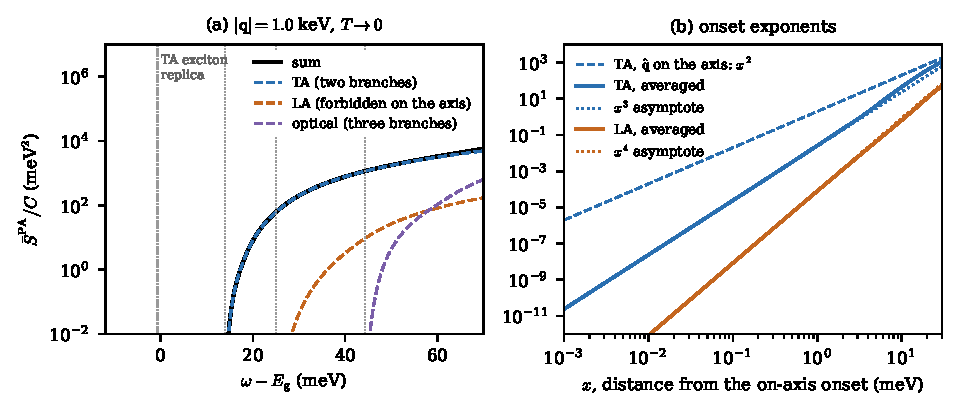
\includegraphics[width=\linewidth]{figures/ch13/fig13_3.pdf}
  \caption{The phonon-assisted structure factor of silicon near its threshold, averaged over the directions of $\vect{q}$ at $|\vect{q}| = \SI{1.0}{keV}$, at zero temperature (emission only), in units of a common coefficient $C$. Model: one valley at $\vect{k}_{\mathrm{c}} = 0.85\,(2\pi/a)$, parabolic pockets and the fixed-$\vect{q}$ form \cref{eq:13.3-near}, with the onset $\Eg + \omega_\nu(\vect{k}_{\mathrm{c}} - \vect{q})$ computed in every direction from the PBE force constants of \cref{sec:5.2}, whose transverse acoustic energy at X is \SI{17.06}{meV} against \SI{18.57}{meV} measured. Every branch is given the same $|M_\nu|^2 = C$, except the longitudinal acoustic one, which is given $C\sin^2\theta_Q$ because its amplitude vanishes on the valley axis; the relative heights are therefore illustrative. The tilt of the pair minimum (at most \SI{0.18}{meV}) is neglected. (a) Components against $\omega - \Eg$: the transverse acoustic edge at \SI{13.98}{meV}, the longitudinal acoustic kink at \SI{25.00}{meV}, and the optical onset at \SI{44.1}{meV}, whose minimum lies far off the axis (dotted lines). The dash-dotted line marks the exciton replica of the transverse acoustic edge, $E_x^b = \SI{14.7}{meV}$ lower, whose strength is not modeled. (b) Each acoustic component against the distance $x$ from its own onset. With $\vect{q}$ held on the axis the transverse acoustic component grows as $x^2$ (dashed). Averaged over directions it grows as $x^3$ (solid), and the longitudinal acoustic one as $x^4$; dotted lines are the asymptotes of \cref{we:13-onset-exp}. The window condition holds over the whole plot: at this $|\vect{q}|$ the zero-phonon pair continuum starts \SI{0.60}{eV} above $\Eg$ (PBE bands of \cref{sec:3.3} with the measured gap).}
  \label{fig:13-paloss}
\end{figure}

The exponents also require the onset itself to lie inside the window. At the onset the pair sits at the band extrema and the phonon takes all of $\vect{Q}^*$, while the zero-phonon edge at the same $\vect{q}$ lies $|\vect{Q}^*|^2/2M_{\mathrm{eh}}$ above $\Eg$ (\cref{eq:3.3-Eminpar}). The window condition $\Eg + \omega_\nu(\vect{Q}^*) \le E_{\mathrm{min}}(\vect{q}) - \delta_{\mathrm{w}}$ then reads $|\vect{Q}^*|^2 - 2M_{\mathrm{eh}}c\,|\vect{Q}^*| - 2M_{\mathrm{eh}}\delta_{\mathrm{w}} \ge 0$ for a branch $\omega_\nu = c|\vect{Q}|$, that is,
\begin{equation*}
  |\vect{Q}^*| \ge M_{\mathrm{eh}}c + \bigl(M_{\mathrm{eh}}^2c^2 + 2M_{\mathrm{eh}}\delta_{\mathrm{w}}\bigr)^{1/2} .
\end{equation*}
With a margin $\delta_{\mathrm{w}} = \SI{0.3}{eV}$, five times the top of the phonon band (\cref{sec:13.6} fixes the margin), and the phase velocity of the transverse acoustic branch at the bound, \SI{5.0}{km.s^{-1}}, the bound is \SI{0.31}{\angstrom^{-1}}, or \SI{0.615}{keV}. In silicon the exponents of \cref{eq:13.3-pon} therefore hold for $|\vect{q}| \le k_{\mathrm{c}} - \SI{0.615}{keV} = \SI{1.33}{keV}$ for parabolic valleys, and for $|\vect{q}| \le \SI{1.27}{keV}$ with the computed bands (\cref{sec:13.6}); over this whole range the transverse acoustic minimum lies on the axis. Closer to the valley the onset falls into the edge band of \cref{sec:13.6}, at the edge of the window, where the phonon-assisted rate is not separately defined and therefore has no exponent of its own.

\begin{workedexample}{The onset exponent from the joint density of states}\label{we:13-onset-exp}
Take silicon at $|\vect{q}| = \SI{1.0}{keV}$, near the valley axis [100], with $k_{\mathrm{c}} = 0.85\,(2\pi/a) = \SI{1.94}{keV}$. On the axis the phonon carries $k_{\mathrm{c}} - q = \SI{0.94}{keV}$, or \SI{0.48}{\angstrom^{-1}} $= 0.41\,\mathrm{X}$, where the computed dispersion of \cref{sec:5.2} gives $\omega_{\mathrm{TA}}(\vect{Q}^*) = \SI{13.98}{meV}$ and $\omega_{\mathrm{LA}}(\vect{Q}^*) = \SI{25.00}{meV}$. The onset $\Eg + \omega_{\mathrm{TA}}(\vect{Q}^*) = \SI{1.184}{eV}$ is reached by dark matter heavier than \SI{0.341}{MeV}, since $qv_{\mathrm{max}} - q^2/2\mchi$ must exceed it with $qv_{\mathrm{max}} = \SI{2.650}{eV}$. The zero-phonon edge at this $\vect{q}$ lies \SI{0.60}{eV} above $\Eg$ on the computed bands of \cref{fig:3-si-bands} (the parabola \cref{eq:3.3-Eminpar} gives \SI{0.73}{eV}), so the window extends to \SI{0.30}{eV} above $\Eg$, well beyond the energies considered here.

\emph{Fixed direction.} With $\vect{q}$ on the axis, \cref{eq:13.3-near} gives $S^{\mathrm{PA}} = Cx^2$ for each transverse acoustic branch, $C = \Omega(m^*_{\mathrm{d}}m_{\mathrm{h}})^{3/2}|M_{\mathrm{TA}}|^2/4\pi^2$, with $m^*_{\mathrm{d}} = 0.322\,m_e$. This is the $x^2$ of \cref{eq:6.5-joint}: the two pockets give six free momenta.

\emph{The curvature of the onset.} The transverse acoustic slope at \SI{0.48}{\angstrom^{-1}} is $\omega_{\mathrm{TA}}' = \SI{16.9}{meV.\angstrom}$, and the first term of \cref{eq:13.3-Eth} is
\begin{equation*}
  \frac{\omega_{\mathrm{TA}}'\,k_{\mathrm{c}}q}{2(k_{\mathrm{c}} - q)} = \SI{16.9}{meV.\angstrom}\times\frac{0.983\times\SI{0.507}{\angstrom^{-2}}}{2\times\SI{0.477}{\angstrom^{-1}}} = \SI{8.85}{meV} .
\end{equation*}
The anisotropy of the branch lowers $\varkappa$. Evaluated on a cone $\theta_q = \SI{0.02}{rad}$ around the axis, the lower transverse acoustic branch has $\varkappa$ between 2.3 and \SI{8.5}{meV} depending on the azimuth $\phi$, the upper one between 18 and \SI{24}{meV}, and the longitudinal acoustic one \SI{16.8}{meV} in every direction. All values of $\varkappa$ are positive: the axis is a minimum.

\emph{The average.} For an onset $\varkappa\theta_q^2$ above its minimum, the average over the sphere of directions, $\bar S = (4\pi)^{-1}\int\dd\phi\,\sin\theta_q\,\dd\theta_q\,S$, is dominated by small $\theta_q$, where $\sin\theta_q \simeq \theta_q$. With $u = \varkappa\theta_q^2$,
\begin{equation*}
  \frac{1}{4\pi}\int_0^{2\pi}\!\dd\phi\int\theta_q\,\dd\theta_q\,C\bigl(x - \varkappa\theta_q^2\bigr)^2\Theta = \frac{C}{4\pi}\int_0^{2\pi}\!\dd\phi\,\frac{1}{2\varkappa}\int_0^x\dd u\,(x - u)^2 = \frac{C\,x^3}{12}\Bigl\langle\frac{1}{\varkappa}\Bigr\rangle_{\!\phi} ,
\end{equation*}
with $\langle 1/\varkappa\rangle_\phi$ the average over the azimuth: \SI{0.240}{meV^{-1}} and \SI{0.047}{meV^{-1}} for the two transverse branches. The exponent has risen from 2 to 3, and $p_{\mathrm{on}} = 3$.

\emph{The forbidden branch.} For the longitudinal acoustic phonon $|M|^2 = C\sin^2\theta_Q \simeq C\,[q/(k_{\mathrm{c}} - q)]^2\theta_q^2$, and the extra $\theta_q^2 = u/\varkappa$ in the integrand gives $\int_0^x u(x - u)^2\dd u = x^4/12$, so
\begin{equation*}
  \bar S_{\mathrm{LA}} = \frac{C\,x^4}{48}\Bigl(\frac{q}{k_{\mathrm{c}} - q}\Bigr)^2\Bigl\langle\frac{1}{\varkappa^2}\Bigr\rangle_{\!\phi} ,
\end{equation*}
and $p_{\mathrm{on}} = 4$.

\emph{The cost of the average.} Per valley, the ratio of the averaged to the on-axis transverse acoustic structure factor is $(x/24)(\langle1/\varkappa\rangle_1 + \langle1/\varkappa\rangle_2)$ for the two branches, $1.2\times10^{-3}$ at $x = \SI{0.1}{meV}$. Only a cone of solid angle $\pi x/\varkappa$ around the valley axis is open, a fraction $x/4\varkappa$ of the sphere.
\end{workedexample}

At fixed $|\vect{q}|$ the halo enters the rate through $q^3\eta(\vmin)\FDM^2$ in \cref{eq:10.2-rate}, which is smooth across an onset as long as $\vmin < v_{\mathrm{max}}$. The spectrum contributed by each $|\vect{q}|$ therefore rises with the same exponent as $\bar L^{\mathrm{PA}}$. The integral over $|\vect{q}|$ smooths the spectrum further, because the onset moves with $|\vect{q}|$; \cref{sec:13.9-onset} combines these factors into the dependence of the rate on the dark-matter mass at the onset.

\section{Screening of the phonon-assisted rate}\label{sec:13.4}

The loss function of \cref{sec:13.3} uses the bare density vertex. At a momentum transfer of \SI{1}{keV} and an energy of \SI{1.2}{eV}, inside the phonon-assisted window, however, the dielectric function of silicon is about 6 in the random-phase approximation (\cref{we:13-external}). The potential that the dark matter exerts on a valence electron is therefore six times weaker than the bare one, and the bare loss function is too large by a factor of 30 to 50. Screening enters the amplitude of \cref{sec:13.2} at three places, among which \cref{sec:8.4} sorted the Coulomb lines: the dark-matter vertex at $(\vect{q},\omega)$, the electron--phonon vertex at $(\vect{Q},\omega_{\vect{Q}\nu})$, and the final pair at $(\vect{q}+\vect{Q}, \omega \mp \omega_{\vect{Q}\nu})$. With all three in the amplitude, the loss function keeps one macroscopic factor $1/\varepsilon_{\mathrm{mac}}(\vect{q},\omega)^2$ and nothing else outside it; \cref{app:D.36} gives the steps at the random-phase level.

\subsection{The screened density and phonon vertices}

The electron--phonon vertex is already screened. Density-functional perturbation theory returns $g_{mn\nu}(\vect{k},\vect{Q})$ as the matrix element of the self-consistent potential change $\partial V_{\mathrm{KS}}$, which is the bare potential of the displaced ions dressed by every Coulomb chain at $\vect{Q}+\vect{G}$, the operator $(1 - f_{\mathrm{Hxc}}R^0)^{-1}$ of \cref{eq:6.2-screen}. These are the vertex lines of \cref{sec:8.4-lines}. The calculation evaluates them at zero frequency, although they carry the phonon frequency; below the gap the error is of relative order $(\omega_{\vect{Q}\nu}/\Eg)^2$, about $3\times10^{-3}$ in silicon (\cref{sec:8.4-lines}). Dividing the computed $g$ once more by $\varepsilon(\vect{Q})$ would count these lines twice, and a bare ionic potential in its place would overstate the long-range part of the coupling by about $\varepsilon_\infty$.

The density vertex of \cref{eq:13.2-M} is bare. The dark matter applies a potential at $(\vect{q},\omega)$, and the electrons that it polarizes add their Hartree and exchange--correlation potentials at every $\vect{q} + \vect{G}$. An electron feels the total, the external potential times the column $(\tilde\varepsilon^{-1})_{\vect{G}0}(\vect{q},\omega)$ of the inverse dielectric matrix of a test electron (\cref{sec:8.7}). These are the external lines, and in the amplitude they replace the density vertex by
\begin{equation}
  \rho^{\mathrm{scr}}_{mn}(\vect{k},\vect{q}) = \sum_{\vect{G}}\bigl(\tilde\varepsilon^{-1}\bigr)_{\vect{G}0}(\vect{q},\omega)\,\rho_{mn}(\vect{k},\vect{q}+\vect{G}) ,
  \label{eq:13.4-rhoscr}
\end{equation}
the vertex of the total potential, as in the screened pair weight \cref{eq:8.7-screened}. The sum over $\vect{G}$ carries the local fields. Without local fields, where the dielectric matrix is diagonal, and without an exchange--correlation kernel, $\rho^{\mathrm{scr}}$ is $\rho/\varepsilon_{\vect{0}\vect{0}}(\vect{q},\omega)$, the head screening of \cref{sec:10.2}.

Exactly one factor of $1/\varepsilon$ survives once the local fields are kept. To see this, remove from the Coulomb kernel its macroscopic term, $v_{\mathrm{C}}(q)$ at $\vect{G} = \vect{G}' = 0$, and let $\bar R$ be the response without it (\cref{sec:4.4}). The full response is then $\bar R$ plus chains of $\bar R$ joined by the macroscopic line, and each element $(\tilde\varepsilon^{-1})_{\vect{G}0}$ factors into $(\varepsilon^{-1})_{\vect{0}\vect{0}} = 1/\varepsilon_{\mathrm{mac}}$ times a local-field column (\cref{app:D.36}). In the random-phase approximation,
\begin{equation}
  \begin{aligned}
  \rho^{\mathrm{scr}}_{mn}(\vect{k},\vect{q}) &= \frac{\rho^{\mathrm{LF}}_{mn}(\vect{k},\vect{q})}{\varepsilon_{\mathrm{mac}}(\vect{q},\omega)} , \\
  \rho^{\mathrm{LF}}_{mn}(\vect{k},\vect{q}) &= \rho_{mn}(\vect{k},\vect{q}) + \sum_{\vect{G}\ne0}v_{\mathrm{C}}(|\vect{q}+\vect{G}|)\,\bar R_{\vect{G}0}(\vect{q},\omega)\,\rho_{mn}(\vect{k},\vect{q}+\vect{G}) ,
  \end{aligned}
  \label{eq:13.4-rhoLF}
\end{equation}
exactly, with $\varepsilon_{\mathrm{mac}}$ the macroscopic dielectric function \cref{eq:4.4-epsmac}. An exchange--correlation kernel adds its own elements, its head included, to the local-field vertex $\rho^{\mathrm{LF}}$ and leaves the factorization intact. Physically, $\rho^{\mathrm{LF}}$ is the bare vertex corrected by the microscopic potentials that the macroscopic field induces inside each cell, and $1/\varepsilon_{\mathrm{mac}}$ is the reduction of the macroscopic field itself. Without local fields $\rho^{\mathrm{LF}} = \rho$ and $\varepsilon_{\mathrm{mac}} = \varepsilon_{\vect{0}\vect{0}}$.

Inside the window this factor is real. No zero-phonon pair exists at $(\vect{q},\omega)$, so the independent-particle response at that momentum and energy has no absorptive part, and $\varepsilon_{\mathrm{mac}}(\vect{q},\omega)$ is real up to the phonon-assisted terms of order $g^2$ that this section computes. We write its zero-phonon value $\varepsilon_1^0(\vect{q},\omega)$, the real part of $\varepsilon_{\mathrm{mac}}$ at $n_g = 0$; its imaginary part $\varepsilon_2^0$ vanishes in the window. The response $R(\vect{q},\omega)$ is then Hermitian, so the retarded column $\delta_{\vect{G}0} + (f_{\mathrm{Hxc}}R)_{\vect{G}0}$ and the advanced one $\delta_{\vect{G}0} + (f_{\mathrm{Hxc}}R^\dagger)_{\vect{G}0}$ coincide, and the question of \cref{sec:8.7}, which of the retarded and advanced weights labels a final pair, does not arise for the external lines. It arises at the pair.

\subsection{The pair channel}

Once the phonon has taken the momentum $\vect{Q}$, the dark matter and the phonon together have disturbed the electrons at a third wavevector, $\vect{q} + \vect{Q}$, and at a third frequency,
\begin{equation*}
  \omega_f = \omega \mp \omega_{\vect{Q}\nu} ,
\end{equation*}
the upper sign for emission. These are the crystal momentum and energy of the final pair itself, $\varepsilon_{c,\vect{k}+\vect{q}+\vect{Q}} - \varepsilon_{v\vect{k}} = \omega_f$ on shell. The disturbance is a density of second order, bilinear in the two vertices, and its Hartree and exchange--correlation potential acts back on the electrons at $(\vect{q}+\vect{Q}+\vect{G},\omega_f)$. That potential can create the final pair directly. Summed over the chains that the medium inserts, it is the pair channel of \cref{sec:8.4-lines}: the Coulomb lines on the segment of the cycle between the two dark-matter vertices. The four-path amplitude of \cref{sec:13.2} leaves it out, because it treats the electrons as independent once the two vertices are given.

To find it we follow the density matrix $\varrho$ of the Kohn--Sham electrons to second order in time-dependent mean-field theory (\cref{app:D.36}). The dark matter acts through the screened vertex, $\mathsf{x} = \rho^{\mathrm{scr}}$ at frequency $\omega$, and the phonon through $\mathsf{y} = g$ at frequency $\mp\omega_{\vect{Q}\nu}$, with the factor $N^{-1/2}(n_{\vect{Q}\nu} + \frac12 \pm \frac12)^{1/2}$ of \cref{eq:13.2-M} taken out. Each field alone produces a first-order density matrix, $\varrho^{\mathsf{x}}_{ab} = \mathsf{x}_{ab}(f_b - f_a)/(\omega - \varepsilon_a + \varepsilon_b + \ii0^+)$ and its analog $\varrho^{\mathsf{y}}$, with $f_a$ the occupation of the one-electron state $a$. At second order, each field acts on the first-order response to the other, which gives the source
\begin{equation*}
  \mathfrak{s}^{(2)}_{ab} = \sum_m\bigl[\mathsf{x}_{am}\varrho^{\mathsf{y}}_{mb} - \varrho^{\mathsf{y}}_{am}\mathsf{x}_{mb} + \mathsf{y}_{am}\varrho^{\mathsf{x}}_{mb} - \varrho^{\mathsf{x}}_{am}\mathsf{y}_{mb}\bigr] ,
\end{equation*}
a matrix over every pair of states, filled or empty. Its element between the final conduction state and the final valence state is, on shell, the four-path amplitude itself, $\mathfrak{s}^{(2)}_{cv} = M^\pm[\rho^{\mathrm{scr}}]$, \cref{eq:13.2-M} with the screened vertex and the unrestricted band sum: the hole paths enter through the occupation differences, and the band-sum theorem of \cref{app:D.35} follows from the density matrix without Fock space.

The source drives a second-order density of the Kohn--Sham electrons at $\vect{q}+\vect{Q}+\vect{G}$,
\begin{equation}
  \delta\nd^{(2)}_{\vect{G}}(\vect{q}+\vect{Q}) = \frac{2}{\Vol}\sum_{\vect{k}}\sum_{ab}\frac{\rho_{ab}(\vect{k},\vect{q}+\vect{Q}+\vect{G})^*\,\mathfrak{s}^{(2)}_{ab}(\vect{k})}{\omega_f + \varepsilon_{b\vect{k}} - \varepsilon_{a,\vect{k}+\vect{q}+\vect{Q}} + \ii0^+} ,
  \label{eq:13.4-dn2}
\end{equation}
the sum running over all pairs of states, including the rearrangements among filled and among empty bands. Its potential is screened by the same chains as any potential at that wavevector and frequency: the electrons respond to it with the bubble $R^0(\vect{q}+\vect{Q},\omega_f)$, their response adds potential, and the series sums to $\tilde\varepsilon^{-1}f_{\mathrm{Hxc}}\,\delta\nd^{(2)}$. In the random-phase approximation $\tilde\varepsilon^{-1}f_{\mathrm{Hxc}} = \varepsilon^{-1}v_{\mathrm{C}}$ is the retarded screened interaction $W^{\mathrm{scr,R}}$ of \cref{eq:4.8-W}. The equation of motion of the pair element $\varrho^{(2)}_{cv}$ is that of a first-order coherence driven at $\omega_f$ by $\mathfrak{s}^{(2)}$ plus this potential, and its numerator is the amplitude for creating the pair. Finally, every term is linear in $\mathsf{x}$, so the factor $1/\varepsilon_{\mathrm{mac}}(\vect{q},\omega)$ of \cref{eq:13.4-rhoLF} comes out in front.
\begin{keyresult}[Screened phonon-assisted amplitude]
In the random-phase approximation and at order $g$ in the amplitude, the screened matrix element of the density into the final state \cref{eq:13.2-final} is $N^{-1/2}(n_{\vect{Q}\nu} + \frac12 \pm \frac12)^{1/2}\,\tilde M^\pm_{cv\nu}(\vect{k},\vect{q},\vect{Q})/\varepsilon_{\mathrm{mac}}(\vect{q},\omega)$. The amplitude without the macroscopic factor is
\begin{equation}
  \begin{split}
  \tilde M^\pm_{cv\nu}(\vect{k},\vect{q},\vect{Q}) &= M^\pm_{cv\nu}\bigl[\rho^{\mathrm{LF}}\bigr] + \sum_{\vect{G}\vect{G}'}\rho_{cv}(\vect{k},\vect{q}+\vect{Q}+\vect{G})\\
  &\quad\times W^{\mathrm{scr,R}}_{\vect{G}\vect{G}'}(\vect{q}+\vect{Q},\omega_f)\,\delta\nd^{(2)}_{\vect{G}'}(\vect{q}+\vect{Q}) ,
  \end{split}
  \label{eq:13.4-Mscr}
\end{equation}
where $M^\pm[\rho^{\mathrm{LF}}]$ is \cref{eq:13.2-M} with the local-field vertex \cref{eq:13.4-rhoLF}, $\delta\nd^{(2)}$ is \cref{eq:13.4-dn2} built with $\mathsf{x} = \rho^{\mathrm{LF}}$, and the retarded $W^{\mathrm{scr,R}}$ carries the index of the final pair first. With an exchange--correlation kernel, $W^{\mathrm{scr,R}}$ becomes $\tilde\varepsilon^{-1}f_{\mathrm{Hxc}}$, and an adiabatic local kernel adds the source of \cref{eq:13.4-kxc}.
\end{keyresult}
\noindent The pair-channel term is added to the four-path term, not multiplied: it does not rescale the four-path term by $1/\varepsilon(\vect{q}+\vect{Q},\omega_f)$, and no $1/|\varepsilon|^4$ appears anywhere. The rate needs \cref{eq:13.4-Mscr} only on shell, where $\mathfrak{s}^{(2)}_{cv}$ equals the four-path amplitude.

\Cref{fig:13-screening} shows the three kinds of screening as diagrams. With the external chains at $(\vect{q},\omega)$, the static chains inside $g$ and the pair chain at $(\vect{q}+\vect{Q},\omega_f)$, every random-phase diagram with one phonon in the final state is counted once (\cref{sec:8.4-lines}). The classification is by the position of a line on the diagram, so it holds where the momentum labels coincide.

\begin{figure}[tbp]
  \centering
  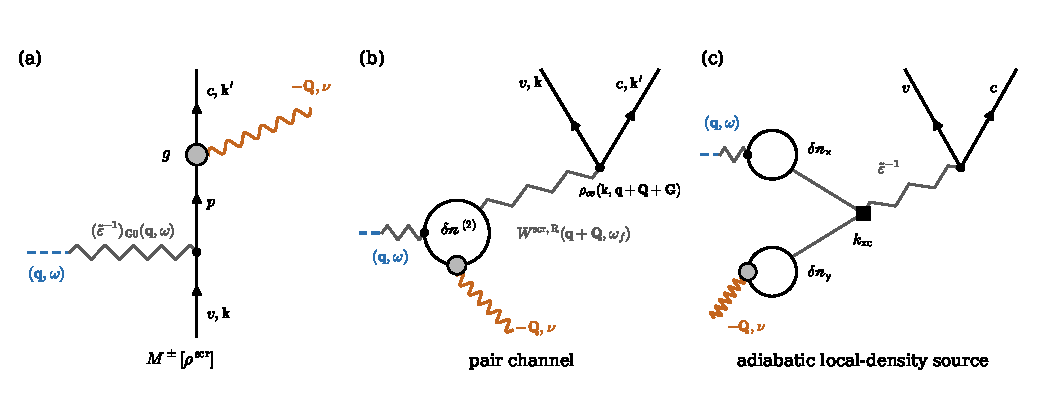
\includegraphics[width=\linewidth]{figures/ch13/fig13_4.pdf}
  \caption{Screening of the phonon-assisted amplitude, schematic. Time runs upward; solid lines are electrons and holes, dashed blue lines the dark-matter potential, wavy lines the phonon, and zigzag lines Coulomb chains summed to all orders. (a) The four-path term $M^\pm[\rho^{\mathrm{scr}}]$: the dark-matter potential reaches the electron through the external chains at $(\vect{q}+\vect{G},\omega)$, the column $(\tilde\varepsilon^{-1})_{\vect{G}0}(\vect{q},\omega)$, and the phonon through the vertex $g$ of density-functional perturbation theory (gray disk), whose chains at $(\vect{Q}+\vect{G},\approx0)$ are inside it. One of the four paths is drawn. (b) The pair channel: the two vertices act on a loop of Kohn--Sham electrons and produce the second-order density $\delta\nd^{(2)}$ at $(\vect{q}+\vect{Q}+\vect{G}',\omega_f)$, whose potential, screened by $W^{\mathrm{scr,R}}(\vect{q}+\vect{Q},\omega_f)$, creates the final pair through $\rho_{cv}(\vect{k},\vect{q}+\vect{Q}+\vect{G})$. (c) The extra source of an adiabatic local-density kernel: the first-order densities induced by the dark matter and by the phonon meet at one point through $k_{\mathrm{xc}}$, the third derivative of the exchange--correlation energy, and the potential they produce is screened at the pair. In the random-phase approximation panel (c) is absent.}
  \label{fig:13-screening}
\end{figure}

The pair line is complex. The final pair is on shell, so pairs exist at $(\vect{q}+\vect{Q},\omega_f)$, and the response there has an absorptive part. With an absorptive interaction the share of the total rate that each final pair receives depends on whether the retarded or the advanced interaction is used, while the total does not. The pair that the cascade receives is the out-state of the evolution, and it takes the retarded $W^{\mathrm{scr,R}}$, as the external weight did in \cref{sec:8.7}.

The momentum of the pair channel is pinned. At the threshold the hole sits near the valence maximum at $\mathrm{\Gamma}$ and the electron near the bottom of a valley at $\vect{k}_{\mathrm{c}}$. The pair momentum $\vect{q}+\vect{Q}$ therefore equals $\vect{k}_{\mathrm{c}}$ up to a reciprocal-lattice vector, whatever $\vect{q}$ is, exactly at the onset and within a few tenths of an inverse \si{\angstrom} at the top of the window. In silicon $|\vect{k}_{\mathrm{c}}| = 0.85\,(2\pi/a) = \SI{1.94}{keV}$, and $\omega_f$ lies within a few tenths of an eV of the gap. One screened interaction, at the six valley momenta and a narrow band of energies, serves the whole window; it is the same one that screens phonon-assisted optical absorption, where $\vect{q} = 0$ and the pair momentum is $\vect{Q}$ (\cref{sec:13.5}). Only $\delta\nd^{(2)}$ depends on $\vect{q}$.

Two limits can be solved, and they show what the pair channel does. In the first, the applied-potential limit, the source acts on every pair at $\vect{q}+\vect{Q}$ as an applied potential would, $\mathfrak{s}^{(2)}_{ab}$ proportional to $\rho_{ab}(\vect{k},\vect{q}+\vect{Q})(f_b - f_a)$. Then $\delta\nd^{(2)}$ is the bubble times that potential, and the two terms of \cref{eq:13.4-Mscr} combine into the source screened as an external potential at the pair's own momentum and energy, $\tilde M^\pm = M^\pm[\rho^{\mathrm{LF}}]/\varepsilon(\vect{q}+\vect{Q},\omega_f)$ without local fields (\cref{app:D.36}). In this limit the pair channel reduces the rate by $1/\varepsilon_1(\vect{k}_{\mathrm{c}},\omega_f)^2$, the screening of the final pair's own momentum.

In the second limit the phonon is a rigid translation of the crystal, $\vect{Q} = 0$, and the vertex is the commutator of the electron momentum with the Kohn--Sham Hamiltonian (\cref{eq:6.2-asr}). In the frame that moves with the nuclei the dark-matter potential only acquires a phase factor, and the displaced density is screened at the energy of the final pair, $1/\varepsilon(\vect{q},\omega_f)$. The four-path term alone gives $1/\varepsilon(\vect{q},\omega)$, screened at the energy deposited, and the pair channel supplies exactly the difference, $1/\varepsilon(\vect{q},\omega_f) - 1/\varepsilon(\vect{q},\omega)$ (\cref{app:D.36}). In the strict limit an acoustic $\omega_{\vect{Q}\nu}$ vanishes, $\omega_f = \omega$, and the pair term vanishes with it. Evaluated with the transverse acoustic energy of the window instead, the two energies change $\varepsilon_1$ of silicon by $1\times10^{-3}$ and the rate by $2\times10^{-3}$ (\cref{we:13-external}). The limit therefore tests the sign and the normalization of \cref{eq:13.4-Mscr}, not its size. It requires a zero-phonon pair at $(\vect{q},\omega_f)$ and therefore lies outside the window. Inside it, the phonons that carry the missing momentum have wavevectors near the zone boundary, where the displacement is not a translation of anything, and the pair channel is neither of these limits.

\subsection{The screened phonon-assisted loss function}

The rate follows from the screened amplitude as it followed from the bare one in \cref{sec:13.3}: the golden rule into the bare pairs, summed over $\vect{k}$, $\vect{Q}$, bands, branches and spin. That this sum is the whole absorptive part of the one-phonon response, with nothing counted twice, is the optical theorem of the mean-field evolution: cut at the pair, the diagrams with both dark-matter vertices on one loop give $|M^\pm[\rho^{\mathrm{LF}}]|^2$, and those with a pair segment the cross terms and the square of the pair channel, which together make $|\tilde M^\pm|^2$ pair by pair (\cref{app:D.36}). The amplitude therefore enters \cref{eq:13.3-LPA} with $M^\pm \to \tilde M^\pm/\varepsilon_{\mathrm{mac}}(\vect{q},\omega)$.

Write $\varepsilon_{\mathrm{mac}} = \varepsilon_1^0 + \delta\varepsilon_1 + \ii\varepsilon_2$, where $\delta\varepsilon_1$ and $\varepsilon_2$ are the phonon-assisted parts, both of order $g^2$ because $\varepsilon_2^0 = 0$. Then $|\varepsilon_{\mathrm{mac}}|^{-2} = (\varepsilon_1^0)^{-2}[1 + O(g^2)]$, and since $|\tilde M^\pm|^2$ is already of order $g^2$, every correction is of order $g^4$, the next order of the expansion in \cref{sec:8.5}.
\begin{keyresult}[Screened phonon-assisted loss function]
Inside the off-shell window, where $\varepsilon_2^0(\vect{q},\omega) = 0$,
\begin{equation}
  \begin{aligned}
  L^{\mathrm{PA}}(\vect{q},\omega) &= \frac{\varepsilon_2^{\mathrm{PA}}(\vect{q},\omega)}{\varepsilon_1^0(\vect{q},\omega)^2} + O(g^4) , \\
  \varepsilon_2^{\mathrm{PA}}(\vect{q},\omega) &= \frac{8\pi^2\alpha}{\Omega\,q^2}\,\Bigl\langle\!\Bigl\langle\sum_{\nu cv\pm}w_\pm\,\bigl|\tilde M^\pm_{cv\nu}\bigr|^2\,\delta\bigl(\varepsilon_{c,\vect{k}+\vect{q}+\vect{Q}} - \varepsilon_{v\vect{k}} \pm \omega_{\vect{Q}\nu} - \omega\bigr)\Bigr\rangle\!\Bigr\rangle ,
  \end{aligned}
  \label{eq:13.4-Lscr}
\end{equation}
with $\tilde M^\pm$ of \cref{eq:13.4-Mscr}, the weights $w_\pm$ of \cref{eq:13.3-LPA}, and $\varepsilon_1^0$ the macroscopic zero-phonon dielectric function with local fields. The rate is \cref{eq:10.2-rate} with $\bar L$ replaced by the direction average $\bar L^{\mathrm{PA}}$.
\end{keyresult}
\noindent From here on $L^{\mathrm{PA}}$ denotes this screened loss function; the function of \cref{eq:13.3-LPA} is its independent-particle value. The definition of $\varepsilon_2^{\mathrm{PA}}$ in \cref{eq:13.4-Lscr} identifies it as the imaginary part, at order $g^2$, of the macroscopic dielectric function, since $L = \Imag(-1/\varepsilon_{\mathrm{mac}}) = \varepsilon_2/|\varepsilon_{\mathrm{mac}}|^2$ must agree with the golden-rule sum term by term. \Cref{eq:13.4-Lscr} is therefore the familiar $L = \varepsilon_2/|\varepsilon|^2$ of \cref{sec:4.4}, evaluated where the zero-phonon $\varepsilon_2$ vanishes and the phonon-assisted one is small.

\Cref{eq:13.4-Lscr} has two simpler forms. One drops the pair channel and the local fields: then $\tilde M^\pm = M^\pm$, $\varepsilon_2^{\mathrm{PA}}$ is the independent-particle loss function of \cref{sec:13.3}, $\varepsilon_1^0 = \varepsilon_{1,\vect{0}\vect{0}}$, and the screened loss function is the unscreened one divided by $\varepsilon_{1,\vect{0}\vect{0}}(\vect{q},\omega)^2$. This is the form that a calculation with the bare density vertex and a scalar dielectric function would use. Each of the two omissions is a definite set of diagrams, and neither is a choice of convention. The other is the optical limit: as $\vect{q} \to 0$, $\varepsilon_1^0$ becomes the optical $\varepsilon_1(\omega)$ and $\varepsilon_2^{\mathrm{PA}}$ the phonon-assisted absorption of \cref{sec:6.5}, now with the pair channel inside it (\cref{sec:13.5}). A measured absorption edge contains the screening of the amplitude, the local-field wings and the pair channel, at $\vect{q} = 0$; the external factor is not in $\varepsilon_2$, and a rate normalized to the edge calibrates it only through the value of $\varepsilon_1^0$ at $\vect{q} \to 0$. Because the pair momentum is pinned at $\vect{k}_{\mathrm{c}}$, the measured edge tests the same screened interaction that acts at finite $\vect{q}$. It does not test the second-order density $\delta\nd^{(2)}$ at finite $\vect{q}$, which is where the two differ.

Outside the window \cref{eq:13.4-Lscr} fails twice. Where zero-phonon pairs exist at $(\vect{q},\omega)$, $\varepsilon_2^0$ is of order one and enters the denominator, and the external lines become absorptive, so that their retarded and advanced weights differ pair by pair. The one-phonon sideband is then no longer a separate quantity, and its treatment by the Dyson convention and the Fano term of \cref{sec:8.6} is the subject of \cref{sec:13.6}.

The prescriptions of \cref{sec:13.3} carry over. A computed $L^{\mathrm{PA}}$ is never added to a measured loss function, and a phonon-assisted table in the normalization of the crystal form factor adds to $|f_{\mathrm{crys}}|^2$ only if both are screened at the same level. A rate that uses \cref{eq:13.4-Lscr} without the pair channel sits at $\mathcal{X}$ = RPA with local fields for the external lines and $\mathcal{X}$ = IP for the pair, and it should be reported that way.

\subsection{The adiabatic local-density source}

The random-phase approximation is linear in the induced density: the Hartree potential of a density $\delta\nd$ is $v_{\mathrm{C}}\,\delta\nd$, whatever its order. The exchange--correlation potential is not. The adiabatic local-density approximation of \cref{sec:4.6} takes $v_{\mathrm{xc}}$ as a function of the density at each point, and expanding it to second order,
\begin{equation}
  v_{\mathrm{xc}}\bigl(\nd_{\mathrm{gs}} + \delta\nd\bigr) = v_{\mathrm{xc}}(\nd_{\mathrm{gs}}) + f_{\mathrm{xc}}\,\delta\nd + \tfrac12k_{\mathrm{xc}}\,\delta\nd^2 + \cdots , \qquad
  k_{\mathrm{xc}}(\vect{r}) = \frac{\dd^3\bigl[\nd\,\varepsilon_{\mathrm{xc}}(\nd)\bigr]}{\dd\nd^3}\bigg|_{\nd_{\mathrm{gs}}(\vect{r})} ,
  \label{eq:13.4-kxc}
\end{equation}
with $f_{\mathrm{xc}}$ the kernel of \cref{eq:4.6-alda} and $k_{\mathrm{xc}}$ the next derivative. The density to first order is the sum of two pieces, $\delta\nd_{\mathsf{x}}$ induced by the dark matter at $(\vect{q},\omega)$ and $\delta\nd_{\mathsf{y}}$ induced by the phonon at $(\vect{Q},\mp\omega_{\vect{Q}\nu})$, the density response that density-functional perturbation theory computes along with $g$. The square $\frac12(\delta\nd_{\mathsf{x}} + \delta\nd_{\mathsf{y}})^2$ contains the cross term $\delta\nd_{\mathsf{x}}\delta\nd_{\mathsf{y}}$ with coefficient one. In real space it is a product, so its Fourier components lie at $\vect{q}+\vect{Q}+\vect{G}$, and it oscillates at $\omega_f$. It is a potential at the pair's momentum and energy that no Coulomb chain produces: the second-order source of the kernel itself. The electrons screen it as any applied potential, and it adds
\begin{equation*}
  \sum_{\vect{G}}\rho_{cv}(\vect{k},\vect{q}+\vect{Q}+\vect{G})\,\bigl[\tilde\varepsilon^{-1}(\vect{q}+\vect{Q},\omega_f)\,\bigl(k_{\mathrm{xc}}\,\delta\nd_{\mathsf{x}}\delta\nd_{\mathsf{y}}\bigr)\bigr]_{\vect{G}}
\end{equation*}
to $\tilde M^\pm$ (\cref{app:D.36}), with $\delta\nd_{\mathsf{x}}$ taken without its macroscopic factor, as $\rho^{\mathrm{LF}}$ is. The term is the reason \cref{eq:13.4-Mscr} is stated at the random-phase level. A calculation that takes $g$ from density-functional perturbation theory in the local-density approximation, and the screening from the adiabatic kernel, has $f_{\mathrm{xc}}$ in every linear chain and is consistent only if it keeps this source too.

Its size follows from exchange alone, with $k_{\mathrm{x}} = -\frac23 f_{\mathrm{x}}/\nd$ and the gas value $f_{\mathrm{x}} = -e^2/4k_{\mathrm{F}}^2$ of \cref{sec:4.6} (\cref{app:D.36}). Against the Hartree part of the pair channel, the new term is
\begin{equation*}
  \frac23\Bigl(\frac{|\vect{k}_{\mathrm{c}}|}{2k_{\mathrm{F}}}\Bigr)^2\,\frac{|\delta\nd_{\mathsf{x}}\delta\nd_{\mathsf{y}}|}{\nd\,|\delta\nd^{(2)}|} ,
\end{equation*}
where the last ratio, a product of two first-order densities over the density times a second-order one, is of order one in the electron gas. The valence electrons of silicon, 32 in a cubic cell of \SI{5.431}{\angstrom}, have $\nd = \SI{0.200}{\angstrom^{-3}}$ and $k_{\mathrm{F}} = \SI{1.81}{\angstrom^{-1}}$, and with $|\vect{k}_{\mathrm{c}}| = \SI{0.983}{\angstrom^{-1}}$ the prefactor is $\frac23\times0.074 = 0.05$. The adiabatic source is therefore an estimated twentieth of the pair channel, times a coefficient of order one that is not known. It matters only as much as the pair channel does.

\subsection{Screening factors in silicon}

The external factor is the largest and the best known, and \cref{we:13-external} sizes it at $|\vect{q}| = \SI{1}{keV}$. It changes by less than \SI{5}{\percent} across the window at fixed $|\vect{q}|$, since $\varepsilon_1$ rises slowly toward the direct gap. It does change with $|\vect{q}|$, however, since the valence electrons screen less at shorter wavelengths: without local fields the static value falls from 10.2 at $\vect{q} \to 0$ to 6.1--6.6 at \SI{1}{keV} and to 3.2--3.7 near \SI{2}{keV} in the same data. A rate integrated over $|\vect{q}|$ therefore needs $\varepsilon_1^0$ at every $|\vect{q}|$, not one number.

Two ratios measure what the simpler forms leave out. The local-field ratio $1 + \delta_{\mathrm{LF}}$ is $L^{\mathrm{PA}}$ with local fields but without the pair channel, divided by $L^{\mathrm{PA}}$ with the head alone. The pair-channel ratio $1 + \delta_{\mathrm{pair}}$ is $L^{\mathrm{PA}}$ with local fields and the pair channel, divided by $L^{\mathrm{PA}}$ with local fields alone. The full screened loss function is then the head-screened one times $(1 + \delta_{\mathrm{LF}})(1 + \delta_{\mathrm{pair}})$. The local-field ratio has two parts. The macroscopic factor changes from $1/\varepsilon_{1,\vect{0}\vect{0}}^2$ to $1/\varepsilon_{\mathrm{mac}}^2$, an increase of 25 to \SI{31}{\percent} at \SI{1}{keV} in the data of \cref{we:13-external}. The vertex changes from $\rho$ to $\rho^{\mathrm{LF}}$, whose wing terms $\vect{G} \neq 0$ the published dielectric functions do not contain. They need the column $\bar R_{\vect{G}0}(\vect{q},\omega)$ and the vertices $\rho_{cv}(\vect{k},\vect{q}+\vect{G})$ at the same $(\vect{q},\omega)$; a bound from the zero-phonon vertices alone, \cref{eq:E.16-dLF}, costs about ten core-hours. The macroscopic factor and the column $(\tilde\varepsilon^{-1})_{\vect{G}0}(\vect{q},\omega)$ are standard outputs of a random-phase calculation with local fields, specified for the phonon-assisted grid in \cref{app:E.14}.

The size of the pair channel in silicon is open, and the two solvable limits of \cref{eq:13.4-Mscr} bracket it only loosely. If the source acted like an applied potential at the pair momentum, the rate would fall by $1/\varepsilon_1(\vect{k}_{\mathrm{c}},\omega_f)^2$. The same data have four mesh points between 1.87 and \SI{2.03}{keV}. At \SI{1.2}{eV} their $\varepsilon_1$ is 3.3 to 3.8 without local fields and 2.9 to 3.5 with them, so that factor is 0.07 to 0.12; the imaginary part there is about $10^{-3}$, since the final pairs sit at their own edge. If the source were the displacement of a rigid crystal, the pair channel would change the rate by $2\times10^{-3}$ at the phonon energy of the window. Neither limit is a bound on the real case, and the sign of $\delta_{\mathrm{pair}}$ is not derived: the source of a zone-boundary phonon is partly a displacement of the bond charge and partly a change of its shape, and the two limits stand for these.

Where the number comes from is known. The screened interaction is needed only at the six valley momenta, $W^{\mathrm{scr,R}}(\vect{k}_{\mathrm{c}},\omega_f)$. The second-order density $\delta\nd^{(2)}$ is a mixed second derivative of the density, with respect to the dark-matter potential and to a phonon displacement, of the kind that density-functional perturbation theory computes for Raman tensors. The route that contains every class at once is a supercell displaced along a phonon pattern, with local fields in the supercell basis: then $\vect{Q}$ is a reciprocal vector of the supercell, and the pair channel is a local-field effect of the supercell. Three runs of that calculation give $\delta_{\mathrm{LF}}$ and $\delta_{\mathrm{pair}}$ separately (\cref{app:E.16}).

The remaining classes are small. The static evaluation of $g$ errs by $3\times10^{-3}$, and the ionic part of the dielectric function, which a silicon crystal has only through its quadrupoles, enters the external and pair chains below $10^{-4}$ (\cref{sec:8.4-lines}).

\begin{workedexample}{The external screening factor in silicon at 1 keV}\label{we:13-external}
Take $|\vect{q}| = \SI{1.0}{keV}$ and $\omega = \SI{1.20}{eV}$, just above the transverse acoustic onset at \SI{1.184}{eV} and well inside the window, which extends to \SI{1.47}{eV} at this momentum (\cref{we:13-onset-exp}). The random-phase dielectric function of silicon with and without local fields has been published on a mesh of $|\vect{q}|$ and $\omega$~\cite[Sect.~III\,B]{knapen2021dark}, with the data files of Ref.~\cite{knapen2022darkelf}. Each mesh momentum is the length of one vector $\vect{q} + \vect{G}$, and so one direction. Two mesh points lie within \SI{0.1}{keV} of \SI{1}{keV}, at 0.944 and \SI{0.986}{keV}, and we quote the range over the two rather than a fit. Interpolating linearly in $\omega$ between the mesh energies 1.04 and \SI{1.26}{eV},
\begin{equation*}
  \varepsilon_{1,\vect{0}\vect{0}} = 6.31\text{--}6.93 , \qquad \varepsilon_{\mathrm{mac}} = 5.52\text{--}6.20 ,
\end{equation*}
and $\varepsilon_2 = 0$ at both, as it must be below the zero-phonon edge.

\emph{The factor.} The screened loss function is the independent-particle one divided by $\varepsilon_1^2$, so the factor is
\begin{equation*}
  \frac{1}{\varepsilon_{1,\vect{0}\vect{0}}^2} = 0.021\text{--}0.025 , \qquad \frac{1}{\varepsilon_{\mathrm{mac}}^2} = 0.026\text{--}0.033 .
\end{equation*}
The unscreened $L^{\mathrm{PA}}$ of \cref{sec:13.3} overstates the screened one by a factor of 40 to 48 with the head alone and 30 to 38 with the macroscopic function. The local fields of the macroscopic function raise the factor by $(\varepsilon_{1,\vect{0}\vect{0}}/\varepsilon_{\mathrm{mac}})^2 = 1.25$ and 1.31 at the two points.

\emph{Against the optical constant.} The measured $\varepsilon_\infty = 11.7$ (\cref{sec:4.4}) would give $1/\varepsilon_\infty^2 = 0.0073$, too small by a factor of 2.9 to 3.4 against the head and 3.6 to 4.5 against the macroscopic function. Screening at \SI{1}{keV} is weaker than at $\vect{q} \to 0$, because the momentum transfer resolves the bonds that do the screening. The same data give 10.2 at $\vect{q} \to 0$ without local fields and 9.1 with them, 13 and \SI{22}{\percent} below the measured value. With bands scissored to the measured gap, that deficit is mostly the electron--hole attraction, the vertex correction that the random-phase approximation leaves out, and the factor at \SI{1}{keV} carries an error of the same kind, which no measurement at this momentum checks.

\emph{Across the window.} Between the onset, \SI{1.184}{eV}, and the window edge, \SI{1.47}{eV}, the factor changes by 4.2 and \SI{4.8}{\percent} at the two points with the head, and by 3.7 and \SI{4.4}{\percent} with the macroscopic function.

\emph{The energy of the final pair.} The logarithmic slope $\dd\ln\varepsilon_1/\dd\ln\omega$ is 0.07 to 0.08 here. Replacing $\omega$ by $\omega_f = \omega - \omega_{\mathrm{TA}}(\vect{Q}^*)$, with $\omega_{\mathrm{TA}}(\vect{Q}^*) = \SI{14.0}{meV}$ at this momentum, changes $\varepsilon_1$ by $0.08\times0.014/1.2 = 1\times10^{-3}$ and the factor by $2\times10^{-3}$, the size that the rigid-translation form of the pair channel takes at this phonon energy.
\end{workedexample}

Whether the pair-channel ratio is the same at finite $\vect{q}$ as at $\vect{q} = 0$ decides how much of it a measured absorption edge calibrates (\cref{sec:13.5}). In both solvable limits it is: the applied-potential factor $1/\varepsilon_1(\vect{k}_{\mathrm{c}},\omega_f)^2$ is the same at every $\vect{q}$, since the pair momentum is pinned, and changes by less than $4\times10^{-4}$ between the phonon energies of the window and of the optical edge, while the rigid-translation term stays below $2\times10^{-3}$ at both momenta. That holds at exact pinning, at the onset; above it the pair momenta spread by about \SI{0.2}{keV} around $\vect{k}_{\mathrm{c}}$, where $\varepsilon_1$ changes by several tenths, and the factor cancels only as far as the distributions of final pairs at finite $\vect{q}$ and at $\vect{q} = 0$ match, an unsized residual. Between the limits it is not derived, because $\delta\nd^{(2)}$ depends on $\vect{q}$ through the phonon at $\vect{k}_{\mathrm{c}} - \vect{q}$. A rate normalized to the measured edge therefore needs, beyond the form factor of its vertex, a screening correction relative to that calibration: the external factor of its model dielectric function against the true $\varepsilon_1^0$, the local-field wings at finite $\vect{q}$ against those at $\vect{q} = 0$, and the pair ratio at finite $\vect{q}$ against its optical value. \Cref{sec:13.9} sizes the first two for the silicon estimate, 0.3 to 2.6 together, and leaves the third as an unsized nuisance. Lines inside a loop, the attraction between the electron and the hole of the final pair, lie outside \cref{eq:13.4-Mscr}; they bind the pair into excitons below the edge and enhance it above, and they are the subject of \cref{sec:13.8}.

\section{The optical limit}\label{sec:13.5}

A photon of \SI{1.24}{eV} absorbed in silicon brings a momentum of \SI{1.24}{eV}, five parts in $10^4$ of the reciprocal-lattice scale $2\pi/a = \SI{2.28}{keV}$, so its phonon supplies all of the \SI{1.94}{keV} between hole and electron, while dark matter near the onset mass supplies \SI{0.9}{keV} or more itself (\cref{sec:13.1}). Both processes have the same final states, and the independent-particle loss function $L^{\mathrm{PA}}_{\mathrm{IP}}(\vect{q},\omega)$ of \cref{eq:13.3-LPA} describes both, at different momentum transfers. Its limit $\vect{q}\to0$ is the phonon-assisted absorption $\varepsilon_2^{\mathrm{PA}}(\omega)$ of \cref{eq:6.5-eps2PA}. The measured absorption edge then serves twice. It tests a computed $L^{\mathrm{PA}}$ at one end of its range of $\vect{q}$, and it enters the rate of dark-photon absorption directly, once it has been transferred from the temperature of the measurement to that of a detector.

\subsection{The small-momentum limit}

The limit cannot be taken term by term in the amplitude $M^\pm_{cv\nu}(\vect{k},\vect{q},\vect{Q})$ of \cref{eq:13.2-M}. Its intraband terms carry density vertices that tend to one and cancel at $\vect{q} = 0$ (\cref{eq:13.2-q0}), so the leading term in $q$ is a difference of large terms, each with a different expansion of the bands and vertices. The continuity equation avoids the expansion. For the full Hamiltonian of electrons and nuclei, \cref{eq:4.3-continuity} gives $[H, n_e(\vect{q})] = \vect{q}\cdot\vect{j}_e(\vect{q})$, exactly, and between any two eigenstates of $H$
\begin{equation*}
  (E_f - E_i)\,\langle f|n_e(\vect{q})|i\rangle = \langle f|\vect{q}\cdot\vect{j}_e(\vect{q})|i\rangle .
\end{equation*}
The second-order amplitude \cref{eq:13.2-T} is a matrix element of this kind. To first order in $H_{\mathrm{ep}}$ the eigenstates of $H$ are $|\tilde i\rangle = |i\rangle + \sum_m|m\rangle\langle m|H_{\mathrm{ep}}|i\rangle/(E_i - E_m)$ and $\langle\tilde f| = \langle f| + \sum_m\langle f|H_{\mathrm{ep}}|m\rangle\langle m|/(E_f - E_m)$, with unchanged energies, because $H_{\mathrm{ep}}$ changes the number of phonons by one and has no diagonal elements. With $E_f = E_i + \omega$, the part of $\langle\tilde f|n_e(\vect{q})|\tilde i\rangle$ linear in $H_{\mathrm{ep}}$ is \cref{eq:13.2-T} term by term. The same construction applied to $\vect{q}\cdot\vect{j}_e(\vect{q})$ gives its second-order amplitude, and the identity holds order by order on the energy shell:
\begin{equation}
  \omega\,\langle f|n_e^{(2)}(\vect{q})|i\rangle = \langle f|\bigl(\vect{q}\cdot\vect{j}_e(\vect{q})\bigr)^{(2)}|i\rangle .
  \label{eq:13.5-ward}
\end{equation}
The intermediate states must be off the shell for the expansion to exist, and the off-shell window of \cref{sec:13.2} guarantees it.

The current needs no cancellation. At $\vect{q} = 0$ it is the total velocity, $\vect{j}_e(0) = \sum_j\vect{p}_j/m_e = \op{\vect{V}}$ of \cref{eq:6.5-HA}, which conserves $\vect{k}$, and its second-order amplitude into the final state of \cref{eq:13.2-final} is the one that \cref{sec:6.5} computed for light, with the photon vertex $(e\mathcal{E}/2\omega)\,\hat{\vect{e}}_\gamma\cdot\op{\vect{V}}$ replaced by $\vect{q}\cdot\op{\vect{V}}$. The same four paths combine into one sum over every band. Write $M^\pm_{cv\nu}(\vect{k},\vect{Q};\hat{\vect{e}}_\gamma)$ for the optical amplitude \cref{eq:6.5-M} with its polarization shown. Then, with $\vect{j}_e(\vect{q}) = \op{\vect{V}} + O(q)$,
\begin{keyresult}[Optical limit of the phonon-assisted amplitude]
\begin{equation}
  M^\pm_{cv\nu}(\vect{k},\vect{q},\vect{Q}) = \frac{q}{\omega}\,M^\pm_{cv\nu}(\vect{k},\vect{Q};\hat{\vect{q}}) + O(q^2) ,
  \label{eq:13.5-Mlim}
\end{equation}
on the energy shell inside the off-shell window, with the final electron at $\vect{k}+\vect{Q}$ in the limit.
\end{keyresult}
\noindent At $\vect{q} = 0$ the right side vanishes, which is \cref{eq:13.2-q0}: the identity contains the cancellation of the intraband terms and needs no expansion of them. It also gives the amplitude its first power of $q$, as \cref{eq:3.2-optical} does for the zero-phonon vertex, with the transition energy $\omega$ in the denominator. For a single pair, $\rho_{cv} \to \vect{q}\cdot\vect{v}_{cv}/\omega$ on the shell; for a pair with a phonon, the velocity vertex is replaced by the whole second-order optical amplitude.

\Cref{eq:4.3-continuity} holds because the potential energy depends on positions alone. A nonlocal pseudopotential breaks this, and $[H, n_e(\vect{q})]$ acquires the commutator of the nonlocal part. The velocity then contains the term $\ii[V_{\mathrm{NL}},\vect{r}]$ of \cref{eq:3.2-dHk}, which first-principles optical calculations include. The electron--phonon vertex of a nonlocal potential, the derivative of $V_{\mathrm{NL}}$ with respect to a displacement, contributes a commutator of the same kind. It is a contact term, in which one vertex creates the phonon and couples to the field at once, and \cref{eq:13.5-ward} holds only if it is kept on the side of the current.

Inserted into the loss function \cref{eq:13.3-LPA}, \cref{eq:13.5-Mlim} multiplies the optical $|M^\pm|^2$ by $q^2/\omega^2$, and the factor $q^2$ cancels the $1/q^2$ of the Coulomb line. The prefactor becomes $8\pi^2\alpha/(\Omega\omega^2) = g_{\mathrm{deg}}\pi e^2/(\omega^2\Omega)$ with $g_{\mathrm{deg}} = 2$ and $e^2 = 4\pi\alpha$. The weights $w_\pm = (1 - \ee^{-\beta\omega})(n_{\vect{Q}\nu} + \frac12 \pm \frac12)$ become $n_{\vect{Q}\nu} + \frac12 \pm \frac12$, since $\beta\omega > 40$ at room temperature for $\omega$ near the gap. The energy delta function loses $\vect{q}$ from the electron's crystal momentum. What remains is \cref{eq:6.5-eps2PA} with the polarization $\hat{\vect{e}}_\gamma = \hat{\vect{q}}$:
\begin{keyresult}[Optical limit of the phonon-assisted loss function]
\begin{equation}
  \lim_{\vect{q}\to0}L^{\mathrm{PA}}_{\mathrm{IP}}(\vect{q},\omega) = \varepsilon_2^{\mathrm{PA}}(\omega)\big|_{\hat{\vect{e}}_\gamma = \hat{\vect{q}}} ,
  \label{eq:13.5-limit}
\end{equation}
for $T \ll \Eg$ and $\omega$ inside the off-shell window at $\vect{q}\to0$, that is, below the direct gap. In a crystal with a center of inversion $L^{\mathrm{PA}}_{\mathrm{IP}}(\vect{q},\omega) = L^{\mathrm{PA}}_{\mathrm{IP}}(-\vect{q},\omega)$, and the corrections are of relative order $q^2$.
\end{keyresult}
\noindent The optical result and its edge are derived in \cref{sec:6.5,app:D.18}. Near threshold, \cref{eq:13.5-limit} reduces to the Hall--Bardeen--Blatt edge \cref{eq:6.5-edge}~\cite{hall1954infrared}, the $q\to0$ form of the fixed-$\vect{q}$ law \cref{eq:13.3-near}. As $\vect{q}\to0$ the phonon wavevector $\vect{Q}^* = \vect{k}_{\mathrm{c}} - \vect{q}$ tends to $\vect{k}_{\mathrm{c}}$, the onset $\Eg + \omega_\nu(\vect{Q}^*)$ tends to the optical threshold $\Eg + \omega_\nu$, and $|M_\nu|^2/q^2$ to the optical $|M_\nu|^2/\omega^2$. The full formula is the one that first-principles calculations of the absorption of silicon evaluate~\cite[Eq.~(1)]{noffsinger2012phonon}.

\subsection{Longitudinal and transverse absorption}

\Cref{eq:13.5-limit} selects the polarization along $\vect{q}$, the longitudinal one. A photon is transverse, and the measured absorption is $\varepsilon_2^{\mathrm{PA}}$ for $\hat{\vect{e}}_\gamma \perp \vect{q}$. Both are projections of one tensor. The amplitude is linear in the polarization, $M^\pm(\vect{k},\vect{Q};\hat{\vect{e}}) = \hat{e}^\alpha M^{\pm\alpha}$, and \cref{eq:6.5-eps2PA} is $\hat{e}^\alpha\hat{e}^\beta\varepsilon_2^{\mathrm{PA},\alpha\beta}(\omega)$, with the tensor built from $M^{\pm\alpha}M^{\pm\beta*}$ under the same double zone average. That average runs over every $\vect{k}$ and $\vect{Q}$ of the zone, every band and every branch, and the thermal state of the phonons is invariant under the point group. The tensor therefore commutes with every operation of the cubic group, and in silicon it is a multiple of the unit matrix (\cref{app:C.3}). The phonon-assisted part obeys \cref{eq:4.4-ET} by itself:
\begin{equation*}
  \varepsilon_2^{\mathrm{PA,T}}(\omega) = \varepsilon_2^{\mathrm{PA,L}}(\omega) = \varepsilon_2^{\mathrm{PA}}(\omega) \qquad (\vect{q}\to0) .
\end{equation*}
The equality holds for the summed tensor, not transition by transition: a single valley and branch contributes an anisotropic tensor, and the six valleys together restore the cubic symmetry.

The measured absorption between the indirect and the direct gap is therefore the longitudinal $\varepsilon_2^{\mathrm{PA}}$ at $\vect{q}\to0$ and at the temperature of the measurement. With the other electrons polarizing the medium, the longitudinal loss function is $\varepsilon_2^{\mathrm{PA}}/(\varepsilon_1^0)^2$ (\cref{eq:13.4-Lscr}). \Cref{eq:13.5-limit} holds for the screened amplitude $\tilde M^\pm$ as well, pair channel included, since the continuity argument uses only the energy shell; the measured $\varepsilon_2^{\mathrm{PA}}$ contains every screening effect of the amplitude at $\vect{q}\to0$, though not the external factor. At the edge of silicon $\varepsilon_1^0 = n_r^2 = 12.8$ at \SI{1.24}{eV}~\cite{franta2017temperature}, and $\varepsilon_2$ stays below $10^{-2}$ within \SI{0.2}{eV} of the gap, so this is the edge part of $\varepsilon_2/|\varepsilon|^2$, the loss function that sets the dark-photon rate \cref{eq:10.7-dp}. A dark photon of mass $m_\phi$ in the halo carries $|\vect{p}_\phi| \approx 10^{-3}m_\phi$, about \SI{1}{meV} at the edge, and sits at $|\vect{p}_\phi|/(2\pi/a) \approx 5\times10^{-7}$. Its longitudinal and transverse modes both absorb with the measured $\varepsilon_2^{\mathrm{PA}}$, and the corrections of order $q^2$ are negligible. Its rate at the edge, with the phonon-assisted absorption of bosonic dark matter in general, is the subject of \cref{sec:13.8}.

\subsection{The measured edge as a test}

\Cref{eq:13.5-limit} turns every measured absorption spectrum of silicon below \SI{3.4}{eV} into a test of a computed $L^{\mathrm{PA}}$ at one end of its domain. The test runs forward: the calculation is done at the temperature of the measurement, with the occupations $n_{\vect{Q}\nu}(T)$ and the gap $\Eg(T)$ of that temperature, and compared with the data. First-principles calculations of the silicon edge at \SIrange{249}{415}{K} agree with the measured spectra at every temperature, once the computed spectra are shifted rigidly by \SIrange{0.15}{0.23}{eV} to correct the computed gap~\cite{noffsinger2012phonon}. The simplest form of the limit is the edge of \cref{eq:6.5-edge} with free pairs, parabolic bands and constant matrix elements. With the branch weights $A_{\mathrm{TA}}:A_{\mathrm{TO}} = 5.5:4.0$ of a fit to the measured edge~\cite{rajkanan1979absorption,stanford2021photoelectric} and one overall scale fitted to the data between 1.18 and \SI{1.30}{eV}, it lies within \SI{15}{\percent} of the measured absorption at \SI{300}{K}~\cite{franta2017temperature} from 55 to \SI{490}{meV} above the gap (\cref{fig:13-transfer}). Closer to the gap the data exceed the edge formula, by a factor of 1.4 at \SI{36}{meV} and of 2 at \SI{17}{meV}; above about \SI{0.5}{eV} the matrix elements and bands vary across the zone, and above \SI{2.5}{eV} new thresholds open.

The constant matrix element is an approximation of the edge formula, not of \cref{eq:13.5-limit}: the full $\varepsilon_2^{\mathrm{PA}}$ keeps $M^\pm$ at every $\vect{k}$ and $\vect{Q}$, and only a calculation of it can follow the data above \SI{0.5}{eV}. Near the gap the excess is the electron--hole attraction, which the independent-particle $L^{\mathrm{PA}}$ leaves out. The bound pair lies $E_x^b = \SI{14.7}{meV}$ below the gap at the crystal momentum of the valley, every threshold has an excitonic companion that much lower (\cref{sec:6.5}), and a calculation that is to match the edge within a few tens of meV must include it (\cref{sec:13.8}).

\subsection{Temperature transfer of absorption data}

The measured edge is also an input. A dark photon absorbed between the indirect and the direct gap of a detector at \SI{10}{mK} sees the phonon-assisted $\varepsilon_2$ of cold silicon. Continuous spectra of the edge are measured at \SI{300}{K} or at \SI{77}{K}; the one measurement below \SI{1}{K} covers a few discrete photon energies from \SI{1.21}{eV} up~\cite{stanford2021photoelectric}. Projections for silicon detectors have used the \SI{77}{K} data near the gap~\cite{hochberg2017absorption}. \Cref{eq:6.5-eps2PA} contains the temperature in two places, the occupations and the gap, and between them they change the edge by large factors (\cref{sec:10.7-edge}).

Take one branch $\nu$ and write $\alpha_{\mathrm{abs},\nu}(\omega;T)$ for its part of the absorption. It consists of an emission component with weight $n_\nu + 1$ and an absorption component with weight $n_\nu$, both functions of the pair energy above the gap, $\omega - \Eg(T) \mp \omega_\nu$. Assume that the spectrum of the pairs, the matrix elements and the phonon energy do not change with temperature, and that the gap moves rigidly by $\Delta E_{\mathrm{g}}(T) = \Eg(T) - \Eg(0) < 0$. At $T \to 0$ only emission survives, and that spectrum is $\alpha^0_{\mathrm{abs},\nu}(\omega)$. At temperature $T$,
\begin{equation}
  \alpha_{\mathrm{abs},\nu}(\omega;T) = (n_\nu + 1)\,\alpha^0_{\mathrm{abs},\nu}\bigl(\omega - \Delta E_{\mathrm{g}}\bigr) + n_\nu\,\alpha^0_{\mathrm{abs},\nu}\bigl(\omega - \Delta E_{\mathrm{g}} + 2\omega_\nu\bigr) ,
  \label{eq:13.5-forward}
\end{equation}
which is \cref{eq:6.5-edge} with a general spectrum in place of the square. The emission term is the cold spectrum moved down by the gap shift; the absorption term is the same spectrum moved down by a further $2\omega_\nu$.

\Cref{eq:13.5-forward} can be solved for the cold spectrum. Evaluate it at $\omega + \Delta E_{\mathrm{g}}$ and divide by $n_\nu + 1$:
\begin{equation*}
  \alpha^0_{\mathrm{abs},\nu}(\omega) = \frac{\alpha_{\mathrm{abs},\nu}(\omega + \Delta E_{\mathrm{g}};T)}{n_\nu + 1} - \frac{n_\nu}{n_\nu + 1}\,\alpha^0_{\mathrm{abs},\nu}(\omega + 2\omega_\nu) .
\end{equation*}
The unknown reappears on the right at an energy higher by $2\omega_\nu$, with the factor $n_\nu/(n_\nu + 1) = \ee^{-\omega_\nu/T}$ of detailed balance (\cref{eq:6.5-ratio}). Substituting the equation into itself and using $1/(n_\nu + 1) = 1 - \ee^{-\omega_\nu/T}$,
\begin{keyresult}[Inverse temperature transfer]
\begin{equation}
  \alpha^0_{\mathrm{abs},\nu}(\omega) = \bigl(1 - \ee^{-\omega_\nu/T}\bigr)\sum_{k=0}^{\infty}\bigl(-\ee^{-\omega_\nu/T}\bigr)^k\,\alpha_{\mathrm{abs},\nu}\bigl(\omega + \Delta E_{\mathrm{g}}(T) + 2k\,\omega_\nu;\,T\bigr) ,
  \label{eq:13.5-inverse}
\end{equation}
exact for the spectrum of one branch measured at the temperature $T$, under the assumptions of \cref{eq:13.5-forward}. The cold absorption is $\sum_\nu\alpha^0_{\mathrm{abs},\nu}$, and the dark-photon rate \cref{eq:10.7-dp} scales with it.
\end{keyresult}
\noindent The series converges geometrically at any temperature, with ratio $\ee^{-\omega_\nu/T}$: 0.064 for the transverse acoustic branch at \SI{77}{K}, $1.7\times10^{-4}$ for the transverse optical one, and 0.49 and 0.11 at \SI{300}{K}. It needs the data up to a few times $2\omega_\nu$ above $\omega$, and it is the unique solution that vanishes below the cold threshold. Each of the assumptions is a property of the spectrum, not of the inversion.

The inversion needs the spectrum of each branch separately, and a measured spectrum is their sum. One spectrum cannot fix two unknown functions. The triangular structure of \cref{eq:13.5-forward} does allow a solution that starts at the lowest threshold and works upward, but the term with the highest argument at each energy is the absorption replica of the transverse optical branch. Each step of that solution divides by its occupation, $n_{\mathrm{TO}} = 1.7\times10^{-4}$ at \SI{77}{K}, and multiplies every error in the data by $\ee^{\omega_{\mathrm{TO}}/T} = 6\times10^3$. At \SI{300}{K} the factor is 9.3. Without spectra resolved by branch, the transfer is therefore ill-posed: the data at one temperature leave the decomposition, and with it the cold spectrum, undetermined. The branch weights must come from elsewhere, from low-temperature spectra in which each threshold is resolved, as in the edge spectroscopy of \cref{sec:6.5}, or from a calculation of $\varepsilon_2^{\mathrm{PA}}$ branch by branch. The cold spectrum inherits their error. From \SI{77}{K} data the inheritance is mild, because only the transverse acoustic branch is occupied: with its weight changed by \SI{25}{\percent} either way, the transferred spectrum changes by less than \SI{1}{\percent} at 15 and \SI{50}{meV} above the cold threshold. From \SI{300}{K} data it changes by $-29$ and $+18$ percent at \SI{15}{meV}.

\begin{figure}[tbp]
  \centering
  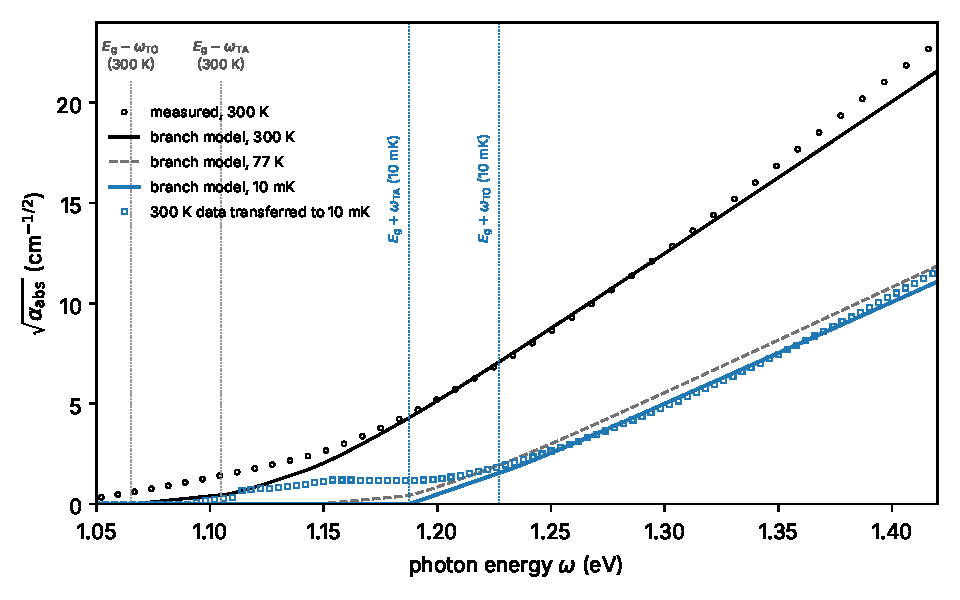
\includegraphics[width=0.92\linewidth]{figures/ch13/fig13_5.pdf}
  \caption{The absorption edge of silicon, as $\sqrt{\alpha_{\mathrm{abs}}}$ against the photon energy, at \SI{300}{K} and transferred to \SI{10}{mK}. Circles: measured at \SI{300}{K}~\cite{franta2017temperature}. Lines: a two-branch model of the edge. It has free pairs with the Hall--Bardeen--Blatt form of \cref{eq:6.5-edge}, $\omega_{\mathrm{TA}} = \SI{18.27}{meV}$ and $\omega_{\mathrm{TO}} = \SI{57.73}{meV}$, branch weights $5.5:4.0$~\cite{rajkanan1979absorption,stanford2021photoelectric}. The gap is the measured $\Eg(T)$ of \cref{sec:6.3}, 1.1692, 1.1652 and \SI{1.1230}{eV} at 0, 77 and \SI{300}{K}, with one scale fitted to the \SI{300}{K} data between 1.18 and \SI{1.30}{eV}. It is drawn at \SI{300}{K} (black), \SI{77}{K} (gray, dashed) and \SI{10}{mK} (blue). Squares: the \SI{300}{K} data transferred to \SI{10}{mK} with \cref{eq:13.5-inverse}, each energy split between the branches in the proportion of the model. Dotted: the thresholds $\Eg - \omega_\nu$ of phonon absorption at \SI{300}{K} and the emission thresholds $\Eg + \omega_\nu$ of cold silicon. Excitonic thresholds, \SI{14.7}{meV} below the free-pair ones, are not modeled.}
  \label{fig:13-transfer}
\end{figure}

\Cref{fig:13-transfer} shows the transfer for silicon. The warm edge starts \SI{57.7}{meV} below the \SI{300}{K} gap of \SI{1.123}{eV}, with the absorption replica of the transverse optical branch, and the cold one at $\Eg(0) + \omega_{\mathrm{TA}} = \SI{1.1875}{eV}$, \SI{0.12}{eV} higher; at \SI{1.236}{eV} the measured \SI{300}{K} absorption, \SI{58}{cm^{-1}}, is 16 times the cold one. Transferred, the data follow the cold model above \SI{1.25}{eV} to within \SI{10}{\percent}, the accuracy with which the model follows the warm data. Below the cold threshold they keep about \SI{1.4}{cm^{-1}}, where cold silicon absorbs nothing outside the excitonic thresholds. That residue is the part of the \SI{300}{K} data that is not of the form \cref{eq:13.5-forward} assumes, the excitonic companions and the thermal broadening of the warm edge, and the inversion carries it to the cold side unchanged in size. Near the cold threshold the transfer of room-temperature data is no better than this residue.

The assumption of a temperature-independent spectrum fails at a level that measurements show. Stanford and co-workers measured the absorption of silicon at 0.5, 5, 77 and \SI{295}{K} and fitted the two-branch form to it with an effective gap of \SI{1.134}{eV}. The fit needs a branch strength that falls with temperature as $\ee^{-c_1T}$ with $c_1 = \SI{1.7e-3}{K^{-1}}$~\cite[Eqs.~(6) and (7)]{stanford2021photoelectric}: a factor 0.61 at \SI{295}{K} and 0.88 at \SI{77}{K}, relative to the lowest temperature, within their own law for the gap, which differs slightly from the one used here. The occupations and a rigid gap do not carry all of the temperature dependence. The bands are renormalized by the lattice vibrations, not only shifted (\cref{sec:6.3}), and the vertices change with them (\cref{sec:13.7}). Transferred with \cref{eq:13.5-inverse}, \SI{295}{K} data therefore underestimate the cold spectrum by about \SI{40}{\percent} on this evidence, and \SI{77}{K} data by about \SI{12}{\percent}, with the opposite sign to the errors of the untransferred data.

\begin{keyresult}[Untransferred \SI{77}{K} data]
Used without transfer, the \SI{77}{K} absorption of silicon overestimates the millikelvin dark-photon rate by the factors
\begin{equation*}
  2.3\text{--}2.6,\quad 1.7\text{--}1.9,\quad 1.3\text{--}1.5,\quad 1.1\text{--}1.3 \qquad \text{at} \qquad x = 15,\ 25,\ 50,\ \SI{100}{meV} ,
\end{equation*}
where $x$ is the energy above the cold threshold $\Eg(0) + \omega_{\mathrm{TA}}$, and by more than a factor of two for $x$ below 18 to \SI{23}{meV}. The upper values hold for the transverse acoustic branch alone and for the two-branch edge to two digits; the lower ones include the measured fall of the branch strength between the lowest temperature and \SI{77}{K}. Untransferred \SI{300}{K} data overestimate the two-branch edge by 38, 16 and 7 at $x = 25$, 50 and \SI{100}{meV}.
\end{keyresult}
\noindent The two causes add. The \SI{77}{K} gap lies \SI{3.97}{meV} below the cold one, so that at the same photon energy the warm emission edge has run $x + \SI{3.97}{meV}$. And the transverse acoustic phonon is still occupied, $n_{\mathrm{TA}} = 0.068$, which adds stimulated emission and an absorption replica that starts $2\omega_{\mathrm{TA}}$ lower. The gap shift dominates close to the threshold, where $(1 + |\Delta E_{\mathrm{g}}|/x)^2$ is large, and the occupation farther away. The factors belong to the free-pair edge, whose power two is the steepest at the threshold. An excitonic edge rises more slowly and its gap-shift factor is smaller. The lower values of the box follow from the branch strength at \SI{77}{K}, lower than the cold one by the factor 0.88 above, which moves the factor of two from $x = 23$ to \SI{18}{meV}. These are the corrections that the silicon dark-photon rate of \cref{sec:10.7-edge} needs near its edge, and they apply to every absorption rate of \cref{chap:10} that uses measured $\sigma_1$ below the direct gap.

\begin{workedexample}{The transverse acoustic correction at 50 meV}\label{we:13-TA-transfer}
Take the transverse acoustic component of the silicon edge at $x = \SI{50}{meV}$ above the cold threshold, $\omega = \Eg(0) + \omega_{\mathrm{TA}} + x = \SI{1.2375}{eV}$, with $\Eg(0) = \SI{1.1692}{eV}$ and $\omega_{\mathrm{TA}} = \SI{18.27}{meV}$, and its \SI{77}{K} spectrum, with $\Eg(\SI{77}{K}) = \SI{1.1652}{eV}$ ($\Delta E_{\mathrm{g}} = \SI{-3.97}{meV}$) and $n_{\mathrm{TA}} = 0.0681$. In the edge form the cold component is $A\,x^2$.

\emph{Forward.} At \SI{77}{K} the emission component has run $\omega - \Eg(\SI{77}{K}) - \omega_{\mathrm{TA}} = \SI{53.97}{meV}$, and the absorption component $\omega - \Eg(\SI{77}{K}) + \omega_{\mathrm{TA}} = \SI{90.50}{meV}$. Relative to the cold value $A\,(\SI{50}{meV})^2$,
\begin{equation*}
  \underbrace{(n_{\mathrm{TA}} + 1)}_{1.0681}\underbrace{\Bigl(\frac{53.97}{50}\Bigr)^2}_{1.1651} + \underbrace{n_{\mathrm{TA}}}_{0.0681}\underbrace{\Bigl(\frac{90.50}{50}\Bigr)^2}_{3.276} = 1.2443 + 0.2230 = 1.467 .
\end{equation*}
The gap shift alone gives \SI{17}{\percent}, stimulated emission multiplies it by 1.068, and the absorption replica adds 0.22: the \SI{77}{K} spectrum is 1.47 times the cold one at this energy.

\emph{Inverse.} \Cref{eq:13.5-inverse} with $\ee^{-\omega_{\mathrm{TA}}/T} = 0.0637$ reads the \SI{77}{K} spectrum at $\omega + \Delta E_{\mathrm{g}} + 2k\omega_{\mathrm{TA}} = 1.2335$, 1.2700, 1.3066, 1.3431, \SI{1.3796}{eV}. In units of the cold value, the terms are
\begin{equation*}
  +1.19087,\quad -0.21547,\quad +0.02724,\quad -0.00289,\quad +0.00028 ,
\end{equation*}
and the partial sums 1.19087, 0.97540, 1.00264, 0.99975, 1.00002. The first term alone, the gap-shifted spectrum divided by $n_{\mathrm{TA}} + 1$, is \SI{19}{\percent} high, because it still contains the absorption replica; the second removes it, and each further term corrects the previous one by a factor $\ee^{-\omega_{\mathrm{TA}}/T}$ and a ratio of squares. Five terms recover the cold value to $2\times10^{-5}$.
\end{workedexample}

\subsection{Finite-momentum corrections}

A dark-matter particle that scatters never reaches the optical limit. To deposit $\omega$ it must transfer at least $q = \omega/v_{\mathrm{max}}$, \SI{0.45}{keV} at the silicon edge with $v_{\mathrm{max}} = 2.65\times10^{-3}$, and in the phonon-assisted window it transfers \SIrange{0.9}{1.3}{keV} (\cref{sec:13.1,sec:13.3}), $0.4$ to $0.6$ of $2\pi/a$. At such $\vect{q}$ the corrections of \cref{eq:13.5-limit} are not small, for three reasons outside the reach of optical data. The intermediate states of path A sit at $\vect{k}+\vect{q}$, and their energy moves by an amount of order $q^2/2m_e$, \SI{0.98}{eV} at \SI{1}{keV}, against a distance from the energy shell of $E_{\mathrm{dir}} - \omega \approx \SI{2.2}{eV}$ at the edge. The density vertices $\rho_{pv}(\vect{k},\vect{q})$ depart from their linear form \cref{eq:3.2-optical} on the scale of $2\pi/a = \SI{2.28}{keV}$, and beyond that a reciprocal-lattice vector inside the vertex reaches valleys that no photon reaches, as the class $(2\pi/a)(2,0,0)$ of \cref{sec:13.3} does, with its own selection rules. And the phonon itself is a different one: at $\vect{q} \to 0$ it carries $\vect{k}_{\mathrm{c}}$, where the transverse acoustic branch is at \SI{18.27}{meV}, while at $|\vect{q}| = \SI{1.0}{keV}$ along the valley axis it carries $\vect{k}_{\mathrm{c}} - \vect{q}$, at $0.41\,\mathrm{X}$, and the computed branch is at \SI{13.98}{meV} (\cref{we:13-onset-exp}). The optical edge measures the electron--phonon vertices only at $\vect{Q} \approx \vect{k}_{\mathrm{c}}$.

The optical limit therefore tests the parts of a calculation that do not depend on $\vect{q}$: the bands at the extrema, the gap, the electron--phonon vertices near $\vect{k}_{\mathrm{c}}$, the unrestricted sum over intermediate bands with its intraband terms, and the normalization of \cref{eq:13.3-LPA}. It does not test the finite-$\vect{q}$ density vertex, the Umklapp classes, the local fields or the vertices at $\vect{k}_{\mathrm{c}} - \vect{q}$, and these carry the dark-matter scattering rate. A computed $L^{\mathrm{PA}}(\vect{q},\omega)$ that reproduces the measured edge at the temperature of the measurement has passed a necessary check. The finite-$\vect{q}$ structure has to be controlled by sum rules and convergence tests.

\section{The off-shell window}\label{sec:13.6}

At $|\vect{q}| = \SI{1.0}{keV}$ along the valley axis the cheapest zero-phonon pair of silicon costs \SI{1.77}{eV}, and the phonon-assisted structure factor of \cref{sec:13.3} was written for energies below it. Two kinds of denominators in the amplitude \cref{eq:13.2-M} can become small. Those of path A with an empty band and of path C with a filled band are the distances of virtual zero-phonon pairs from the energy shell, and they vanish as $\omega$ reaches $E_{\mathrm{min}}(\vect{q})$. The intraband terms, path A with $p = c$ and path B with $p = v$, have denominators of order $|\vect{Q}|$ and vanish as the phonon becomes a soft acoustic one, while the interband vertices of that phonon grow as $|\vect{Q}|^{-1/2}$. The soft acoustic phonon produces no divergence: translation invariance fixes its amplitude, and inside the window it is never on the energy shell. The vanishing zero-phonon detunings, however, set the boundary of the region in which the phonon-assisted rate exists as a quantity of its own, with the margin $\delta_{\mathrm{w}}$ of \cref{sec:8.6,sec:13.3}, \SI{0.3}{eV} in silicon.

\subsection{The soft acoustic limit}

A long acoustic wave moves every atom of a region by nearly the same amount, and a uniform displacement of the whole crystal is no excitation. The electron--phonon vertex reflects this only in part. By \cref{eq:6.2-asr} its intraband elements vanish as $\vect{Q}\to0$, but its interband elements tend to $\ii\ell_{\vect{Q}\nu}(\varepsilon_m - \varepsilon_n)\hat{\vect{e}}_\nu\cdot\vect{p}_{mn}$, the rigid translation of the electronic states, and with $\ell_{\vect{Q}\nu} = (2M_{\mathrm{cell}}c_\nu|\vect{Q}|)^{-1/2}$ they grow without bound. In \cref{eq:13.2-M} these large interband terms meet intraband terms of the form $0/0$, a vertex of order $\ell|\vect{Q}|$ over a denominator of order $|\vect{Q}|$. Neither kind can be estimated alone. Translation invariance, which \cref{sec:8.3} wrote as a Ward identity for matrix elements, decides their sum.

The identity we need is \cref{eq:D.37-ward}. Change the vertex by $\delta g_{mn} = (\varepsilon_{m,\vect{\kappa}+\vect{Q}} - \varepsilon_{n\vect{\kappa}} \pm \omega_{\vect{Q}\nu})\mathfrak{t}_{mn}$, the matrix element of a commutator with the unperturbed Hamiltonian, for any one-electron operator $\op{\mathfrak{t}}_{\vect{Q}}$. On the energy shell every term of \cref{eq:13.2-M} then has numerator equal to $\pm$ its denominator, band by band, and the sum over all bands collapses to $\langle c,\vect{k}'|[\op{\mathfrak{t}}_{\vect{Q}},\ee^{\ii\vect{q}\cdot\vect{r}}]|v,\vect{k}\rangle$ (\cref{app:D.37}). The amplitude is unchanged if this contact term is added back. The useful choice of $\op{\mathfrak{t}}_{\vect{Q}}$ carries each electron along with the local displacement of the wave, \cref{eq:D.37-s}. The vertex that remains, the comoving vertex $g^{\mathrm{cm}}$ of \cref{eq:D.37-gcm}, vanishes at $\vect{Q} = 0$ for every pair of bands, by \cref{eq:6.2-asr}. Its first order in $\vect{Q}$ is the coupling to a uniform strain, the deformation-potential tensor $D^n$ of \cref{eq:6.2-D}, plus a coupling to the velocity of the moving lattice. And the contact term is $\ii\ell_{\vect{Q}\nu}(\hat{\vect{e}}_\nu\cdot\vect{q})\,\rho_{cv}(\vect{k},\vect{q}+\vect{Q})$, because the density at wavevector $\vect{q}$ carries momentum $\vect{q}$. With these, the amplitude has a finite limit.
\begin{keyresult}[Soft acoustic limit of the phonon-assisted amplitude]
For an acoustic branch $\nu$ with $\omega_{\vect{Q}\nu} = c_\nu|\vect{Q}|$ and polarization $\hat{\vect{e}}_\nu$, nondegenerate bands $c$ and $v$, and $\hat{\vect{Q}} = \vect{Q}/|\vect{Q}|$, the amplitude \cref{eq:13.2-M} tends on the energy shell to
\begin{equation}
  \begin{split}
  M^\pm_{cv\nu}(\vect{k},\vect{q},\vect{Q}) \to{}& \ii\,\ell_{\vect{Q}\nu}\,\rho_{cv}(\vect{k},\vect{q})
  \biggl[\underbrace{\hat{\vect{e}}_\nu\cdot\vect{q}}_{\text{recoil}}\\
  &+ \underbrace{\frac{\hat{\vect{Q}}\cdot D^c\cdot\hat{\vect{e}}_\nu \mp c_\nu\,\hat{\vect{e}}_\nu\cdot\vect{p}_{cc}}{\hat{\vect{Q}}\cdot\vect{v}^{\mathrm{g}}_c \pm c_\nu}
  - \frac{\hat{\vect{Q}}\cdot D^v\cdot\hat{\vect{e}}_\nu \mp c_\nu\,\hat{\vect{e}}_\nu\cdot\vect{p}_{vv}}{\hat{\vect{Q}}\cdot\vect{v}^{\mathrm{g}}_v \pm c_\nu}}_{\text{deformation and velocity}}\biggr] ,
  \end{split}
  \label{eq:13.6-soft}
\end{equation}
with $D^c$, $\vect{v}^{\mathrm{g}}_c$, $\vect{p}_{cc}$ taken at $\vect{k}+\vect{q}$ and $D^v$, $\vect{v}^{\mathrm{g}}_v$, $\vect{p}_{vv}$ at $\vect{k}$, and the upper sign for emission. The leading term is of order $|\vect{Q}|^{-1/2}$, and the relative correction is of order $|\vect{Q}|$, for $|\vect{Q}|$ small compared with the scale over which the group velocities change; at a band extremum of mass $m^*$ this is $|\vect{Q}| \ll 2m^*c_\nu$.
\end{keyresult}
\noindent The limit is derived in \cref{app:D.37}. The recoil term is the first order in the displacement of $\ee^{\ii\vect{q}\cdot(\vect{r} - \vect{u})}$: the dark matter kicks an electron that rides on the lattice, and the lattice under it recoils. The deformation terms are the soft phonon emitted by the final electron after the kick, or by the hole before it, through the strain it produces; their denominators are the detunings of the zero-phonon pair at $\vect{q}$, which shrink with $|\vect{Q}|$. The velocity terms are smaller than the deformation terms by $c_\nu|\vect{p}_{nn}|/|D^n|$, a few times $10^{-3}$ per band in \cref{we:13-soft} (and $10^{-5}$ there once the electron and hole terms cancel), but they turn the laboratory-frame intraband vertex into the comoving one. That vertex is $\ii\ell|\vect{Q}|\,\hat{\vect{Q}}\cdot(D^n + \vect{v}^{\mathrm{g}}_n\otimes\vect{p}_{nn})\cdot\hat{\vect{e}}_\nu$ (\cref{eq:D.37-Xi}). It reduces to \cref{eq:6.2-D} at a band extremum, and away from one it carries a Galilean term that a frozen-strain calculation does not produce (\cref{app:D.37}).

The soft acoustic limit of \cref{sec:8.3} is a different statement. There the probe itself is proportional to mass and its amplitude vanishes as $q^2$ at fixed energy. Here the probe is the electron density, its momentum $\vect{q}$ is finite, and the soft object is the phonon. Translation invariance does not make the amplitude vanish. It makes it finite, of order $\ell_{\vect{Q}\nu}$ rather than of order $\ell_{\vect{Q}\nu}/|\vect{Q}|$ as the separate intraband terms would suggest, and it fixes its value through $D^n$, the band velocities and $\vect{q}$. The squared amplitude then behaves as $1/|\vect{Q}|$, and with the phase space $Q^2\dd Q$ the emission of soft phonons is integrable, as $Q\,\dd Q$ at $T = 0$ and as $\dd Q$ at finite temperature.

In silicon the deformation terms dominate. With $D \approx \SI{9}{eV}$ along the valley axis (\cref{sec:6.2}) and $c_\nu = \SI{8.43}{km.s^{-1}}$, $D/c_\nu$ is 300 to \SI{350}{keV}, against momentum transfers of 1 to \SI{2}{keV} near the window, so at the band extrema the recoil term is a correction of a percent or less. It is not negligible everywhere. For a nearly free electron the strain shift at fixed reduced wavevector, $D^n$, and the Galilean term $\vect{v}^{\mathrm{g}}_n\otimes\vect{p}_{nn}$ nearly cancel, since a weak electron--ion potential gives a weak electron--phonon vertex. The recoil term is then of the same size as the rest of the bracket. \Cref{we:13-soft} shows such a case.

As a test of a computed amplitude, \cref{eq:13.2-M} is evaluated as a function, with the energy-shell condition imposed but no delta function, and it must approach \cref{eq:13.6-soft} with a deviation linear in $|\vect{Q}|$ for both signs, several directions and decreasing $|\vect{Q}|$. A failure of the test exposes a common shortcut. Codes set the vertices of the three acoustic modes at $\vect{Q} = 0$ to zero (\cref{sec:6.2}), and an interpolation that carries this into the neighborhood of $\vect{Q} = 0$ removes the rigid-translation part of the interband vertices. That part supplies the recoil term and the bare Galilean terms, $\ii\ell[\hat{\vect{e}}_\nu\cdot(\vect{q} - \vect{p}_{cc} + \vect{p}_{vv})]\rho_{cv}$ (\cref{app:D.37}), and in \cref{we:13-soft} its loss changes $|M|^2$ by a factor of ten. Outside the window the zero-phonon pair at $\vect{q}$ is real and \cref{eq:13.6-soft} is its amplitude to emit a soft phonon. The denominators vanish on the cone $\hat{\vect{Q}}\cdot\vect{v}^{\mathrm{g}}_c = \mp c_\nu$, where the electron outruns the sound wave. This is the Cherenkov emission of \cref{eq:6.3-cherenkov}, a real decay of the pair, and it is regularized by the width like the other resonances below.

Inside the off-shell window the soft limit is never reached. A final state at $\omega \le E_{\mathrm{min}}(\vect{q}) - \delta_{\mathrm{w}}$ whose electron sits at $\vect{k}+\vect{q}+\vect{Q}$ needs $\varepsilon_{c,\vect{k}+\vect{q}} - \varepsilon_{c,\vect{k}+\vect{q}+\vect{Q}} \ge \delta_{\mathrm{w}}$, since the pair at $\vect{q}$ costs at least $E_{\mathrm{min}}(\vect{q})$. The electron must therefore fall by $\delta_{\mathrm{w}}$ over the distance $|\vect{Q}|$ in crystal momentum, which bounds the phonon wavevector from below by $\delta_{\mathrm{w}}/(v^{\mathrm{g}}_{\max} + c_\nu)$ (\cref{eq:D.37-Qmin}). The steepest conduction band of silicon on the symmetry lines of \cref{fig:3-si-bands} has a slope of \SI{16.7}{eV.\angstrom}, or \SI{2.5e6}{m.s^{-1}}, and at $\delta_{\mathrm{w}} = \SI{0.3}{eV}$ the bound is \SI{0.018}{\angstrom^{-1}}. The soft limit needs $|\vect{Q}| \ll 2m^*c_\nu$, with $m^*c_\nu = 1.0\times10^{-3}$ and $6.7\times10^{-3}\,\si{\angstrom^{-1}}$ for transverse emission across the valley and longitudinal emission along it. Inside the window the intraband denominators are zero-phonon detunings of at least $\delta_{\mathrm{w}}$, the amplitude has no infrared feature at any temperature, and no subtraction is needed. At the onset itself the phonon is far harder, $|\vect{Q}^*| \ge \SI{0.31}{\angstrom^{-1}}$ (\cref{sec:13.3}). A computation inside the window can therefore give the acoustic modes at $\vect{Q} = 0$ zero weight, as long as it keeps the interband vertices near it.

\begin{workedexample}{The soft-phonon amplitude in a one-dimensional crystal}\label{we:13-soft}
A test of \cref{eq:13.6-soft} needs a vertex computed in the laboratory frame, without the comoving construction, since a model whose orbitals ride on the atoms has the identity built in. Take a chain of rigid ions, lattice constant $a = \SI{3.0}{\angstrom}$, mass \SI{28.09}{\atomicmassunit}, each ion a Gaussian well $-V_0\ee^{-x^2/2\sigma^2}$ with $V_0 = \SI{2.5}{eV}$ and $\sigma = \SI{0.5}{\angstrom}$, and one spinless electron per cell, solved in 41 plane waves. The lowest band is filled and the next empty, with a gap of \SI{1.215}{eV} at the zone boundary. One longitudinal acoustic branch has $c_\nu = \SI{5.0}{km.s^{-1}}$. The vertex is the matrix element of the potential change of ions displaced by $\ell_{\vect{Q}\nu}\ee^{\ii QX_j}$, the density vertex is $\ee^{\ii qx}$, and \cref{eq:13.2-M} is summed over 40 bands. All parameters are illustrative.

Put the hole at $k = 0.80\,\pi/a$ and the transfer at $q = 0.30\times2\pi/a = \SI{0.628}{\angstrom^{-1}}$, away from the band extrema. The pair at $q$ costs \SI{5.68}{eV} and $|\rho_{cv}| = 0.965$. The valence state has $v^{\mathrm{g}}_v = \SI{5.91}{eV.\angstrom}$, 180 times the sound speed, and $p_{vv} = \SI{0.776}{\angstrom^{-1}}$; the conduction state $v^{\mathrm{g}}_c = \SI{11.05}{eV.\angstrom}$ and $p_{cc} = \SI{1.450}{\angstrom^{-1}}$. Straining the crystal at fixed reduced wavevector gives $D^v = \SI{-4.563}{eV}$ and $D^c = \SI{-15.237}{eV}$, nearly the $-2\times$ kinetic energy of free electrons. The laboratory intraband slopes, read off the computed vertex at $|Q| = 10^{-5}\times2\pi/a$, are \SI{0.021}{eV} and \SI{0.774}{eV}, equal to $D^n + v^{\mathrm{g}}_np_{nn}$ to \SI{e-4}{eV}: the strain and Galilean terms cancel to a few percent.

The comoving vertex is of order $\ell|Q|$ for every band pair, about $220\,\ell|Q|$\,eV at most, while the laboratory interband vertex grows from 0.44 to \SI{4.4}{eV} as $|Q|$ falls from $10^{-2}$ to $10^{-4}\times2\pi/a$. For emission with $Q > 0$ the bracket of \cref{eq:13.6-soft} is
\begin{center}
\small
\begin{tabular}{lr}
  \toprule
  term & value ($\si{\angstrom^{-1}}$) \\
  \midrule
  recoil, $q$ & $+0.6283$ \\
  deformation & $-0.6076$ \\
  velocity & $-1.1\times10^{-5}$ \\
  total & $+0.0207$ \\
  \bottomrule
\end{tabular}
\end{center}
and the full amplitude deviates from the limit by 0.20, 0.020 and 0.0020 at $|Q| = 10^{-2}$, $10^{-3}$ and $10^{-4}\times2\pi/a$: linearly, as the relative correction of order $|\vect{Q}|$ requires. The same holds for absorption and for $Q < 0$. Recoil and deformation nearly cancel here, and with the interband vertices set to zero the recoil is lost and $|M|^2$ comes out 10.4 times too large.

At the band extrema the balance changes. With the hole at $k = \pi/a$ and $q = 2\pi/a$, an Umklapp transfer that puts the electron at the bottom of the conduction band, both velocities vanish, $D^v = \SI{-7.42}{eV}$ and $D^c = \SI{-7.26}{eV}$, and the bracket is $q \pm (D^c - D^v)/c_\nu = 2.09 \pm \SI{4.91}{\angstrom^{-1}}$, so that the soft amplitude differs by a factor of 2.5 between the two directions of $\vect{Q}$. The limit is reached only for $|Q| \ll 2m^*c_\nu$, here $1.2\times10^{-3}\,\si{\angstrom^{-1}}$ with $m^* = 0.135\,m_e$, and since each deformation term is about \SI{220}{\angstrom^{-1}} and they cancel to \SI{4.9}{\angstrom^{-1}}, the deviation falls below \SI{1}{\percent} only at $|Q| = 10^{-8}\times2\pi/a$. Setting the interband vertices to zero now removes the recoil term: for emission with $Q > 0$ it halves $|M|^2$, and for the opposite direction it multiplies $|M|^2$ by 2.9. In silicon, where $(D^c - D^v)/c_\nu$ is a hundred times $q$, this effect is at the percent level.
\end{workedexample}

\subsection{The off-shell window}

By \cref{eq:13.2-doff}, the denominators of path A with an empty band and of path C with a filled band are at least $E_{\mathrm{min}}(\vect{q}) - \omega$ in size on the energy shell, and the other two kinds at least $\Eg - \omega_{\vect{Q}\nu}$, which never vanishes. A denominator of \cref{eq:13.2-M} therefore vanishes exactly where a first-order transition at the same $(\vect{q},\omega)$, the creation of a zero-phonon pair by the density alone, is on shell. Below the zero-phonon edge no such transition exists. Above it, at fixed $(\vect{q},\omega)$, the resonance condition is met on a surface of crystal momenta, and the sum over final states crosses that surface. There the squared amplitude has a double pole $1/x^2$ in the detuning $x$, which is not integrable across a simple zero. It has no principal value either; as \cref{sec:2.4} showed, it needs the width of the intermediate state, after which the rate splits into a cascade and a finite part. The second-order rate is then no longer a quantity of its own. Its value depends on the width, and its share of the response depends on a convention.

The edge must be the renormalized one. The bands in the denominators are shifted and broadened by the electron--phonon self-energy (\cref{eq:6.3-ren}), and the pair edge moves with them, by the zero-point renormalization of the gap at low temperature and by more as the temperature rises (\cref{sec:13.7}). A bound pair lies below the free pairs by its binding energy (\cref{sec:13.8}). We write $E^{\mathrm{ren}}_{\mathrm{min}}(\vect{q},T)$ for the lowest energy of a zero-phonon final state at crystal momentum $\vect{q}$, with renormalized bands and the bound pair included, and use the same renormalized energies in the denominators. A bare edge with renormalized denominators, or the reverse, misplaces the boundary by the renormalization itself. In the silicon numbers of this chapter the conduction bands are shifted so that the indirect gap equals the measured one at low temperature, which places the renormalized edge correctly at the band extrema and treats the renormalization as rigid in $\vect{k}$.
\begin{keyresult}[Window theorem]
The phonon-assisted structure factor \cref{eq:13.3-SPA}, built from the amplitude \cref{eq:13.2-M}, is defined at $(\vect{q},\omega)$ without widths, without $\ii0^+$, without subtraction and without counterterms if and only if every first-order transition at the same $(\vect{q},\omega)$ is off shell, $\omega < E^{\mathrm{ren}}_{\mathrm{min}}(\vect{q},T)$, with renormalized energies used in the edge and in the denominators alike. It is quoted as a channel of its own in the pointwise window
\begin{equation}
  \omega \le E^{\mathrm{ren}}_{\mathrm{min}}(\vect{q},T) - \delta_{\mathrm{w}} , \qquad
  \delta_{\mathrm{w}} \gg \omega_{\max},\ \hat\varGamma,\ T ,
  \label{eq:13.6-window}
\end{equation}
applied at each $\vect{q}$ separately, with $\omega_{\max}$ the top of the phonon band and $\hat\varGamma$ the largest width of the zero-phonon pairs between the edge and $\delta_{\mathrm{w}}$ above it. In silicon $\delta_{\mathrm{w}} = \SI{0.3}{eV}$.
\end{keyresult}
\noindent The first half is the statement about the denominators above. The second half is about accuracy, and it needs the resummed amplitude of \cref{sec:8.6}. There the virtual pair $m$ enters through its propagator $\GF_m(\omega) = 1/[\omega - E_m - \Sigma_m(\omega)]$, \cref{eq:8.6-amp}, and the second-order amplitude keeps only $1/(\omega - E_m)$. The difference is of relative order $\Sigma_m(\omega)/(\omega - E_m)$, and the margin must make it small. With renormalized energies the real part of $\Sigma_m$ at the pair's own energy is absorbed into $E_m$, and three pieces remain. The self-energy changes between $E_m$ and $\omega$, on the scale of the phonon energies, because the thresholds for emitting each phonon sit $\omega_{\vect{Q}\nu}$ above the edges of the continuum (\cref{sec:6.3}); this requires $\delta_{\mathrm{w}} \gg \omega_{\max}$. The imaginary part, the width, requires $\delta_{\mathrm{w}} \gg \hat\varGamma$. And thermal phonons broaden the edge by about $T$. The same ratio $\omega_{\vect{Q}\nu}/\delta_{\mathrm{off}}$ sets the error of the adiabatic form (\cref{eq:13.2-err}), and the bound pair adds the condition $\delta_{\mathrm{w}} \gg E_x^{\mathrm{b}}$ unless it is already part of the edge.

The parameter $\theta_{\mathrm{ep}}$ of \cref{eq:8.5-theta} looks like the controlling one, and taken at face value it would forbid a margin of \SI{0.3}{eV}. Evaluated at $\delta_{\mathrm{off}} = \SI{0.3}{eV}$ with the largest vertex of silicon, the optical vertex of the holes, about \SI{0.25}{eV}, it is $(0.25/0.3)^2 \approx 0.7$; the $\theta_{\mathrm{ep}} = 1$ at \SI{0.25}{eV} of \cref{sec:8.5} is a bound of this kind, not a size. But $\theta_{\mathrm{ep}}$ counts one more pair of vertices on intermediate states that all lie $\delta_{\mathrm{off}}$ from the shell. At the window edge the extra vertices act on the virtual pair, whose self-energy sums $|g|^2$ over one-phonon states spread across an energy range $E_{\mathrm{w}}$ of an electronvolt or more, the width of the continuum in the sense of \cref{sec:2.4}. Its size is then $|\Sigma_m| \approx \langle|g|^2\rangle/E_{\mathrm{w}}$ rather than $\langle|g|^2\rangle/\delta_{\mathrm{w}}$, and the relative correction $|\Sigma_m|/\delta_{\mathrm{w}}$ is $\theta_{\mathrm{ep}}\,\delta_{\mathrm{w}}/E_{\mathrm{w}} \approx 0.7\times0.3/1 \approx 0.2$ at \SI{0.3}{eV}. Measured on the gap itself this is the zero-point renormalization over the margin, the correction that the resummation adds.

The silicon numbers fix the margin (\cref{fig:13-offshell}(b)). The top of the phonon band, the zone-center optical phonon of \SI{64.1}{meV}, is 0.21 of \SI{0.3}{eV}, and the transverse acoustic phonon of the onset, \SI{14.8}{meV}, is 0.05. The zero-point renormalization of the gap is \SI{56}{meV} as computed at fixed volume and 71 to \SI{73}{meV} for the electron--phonon part implied by experiment (\cref{sec:6.3}), 0.19 to 0.24 of the margin. It is absorbed into the renormalized edge, and only its variation across the margin remains. The exciton binding energy, \SI{14.7}{meV}, is 0.05. At a detector's temperature $T$ is zero for this purpose; at \SI{300}{K} it would be 0.09.

For the widths we estimate the decay of the pair at the zero-phonon edge by phonon emission, with deformation-potential rates and the constants computed by Li, Graziosi and Neophytou~\cite[Table~III and Eq.~(10)]{li2021deformation}. The electron scatters between valleys by the g-type longitudinal optical and the f-type longitudinal acoustic and transverse optical phonons, the hole emits optical phonons, and both emit acoustic phonons as in \cref{eq:6.3-cherenkov}. The pair at $E_{\mathrm{min}}(\vect{q})$ shares its kinetic energy in proportion to the masses along the valley axis, 0.77 to the electron. Between $|\vect{q}| = 0.4$ and \SI{1.4}{keV} this gives widths of 3 to \SI{21}{meV} at the edge, \SI{11}{meV} at \SI{1.0}{keV}, and \SI{15}{meV} at \SI{1.0}{keV} and \SI{0.3}{eV} above the edge, so that $\hat\varGamma/\delta_{\mathrm{w}}$ stays below 0.1. Every ratio is then below about 0.2. A margin of \SI{0.1}{eV} would put the phonon ratio at 0.64 and the renormalization ratio at 0.56 to 0.73, and one of \SI{0.5}{eV} would bring them to 0.13 and 0.11 to 0.15 but shrink the window: along the valley axis it would end at $|\vect{q}| = \SI{1.07}{keV}$ instead of \SI{1.27}{keV}. The margin is therefore $\delta_{\mathrm{w}} = \SI{0.3}{eV}$, and with it the bound $|\vect{Q}^*| \ge \SI{0.31}{\angstrom^{-1}}$ of \cref{sec:13.3} holds. Inside the window the second-order rate then carries a relative correction of order 0.2 at the edge, falling as $1/(E_{\mathrm{min}} - \omega)$ toward the onset.

\begin{figure}[tbp]
  \centering
  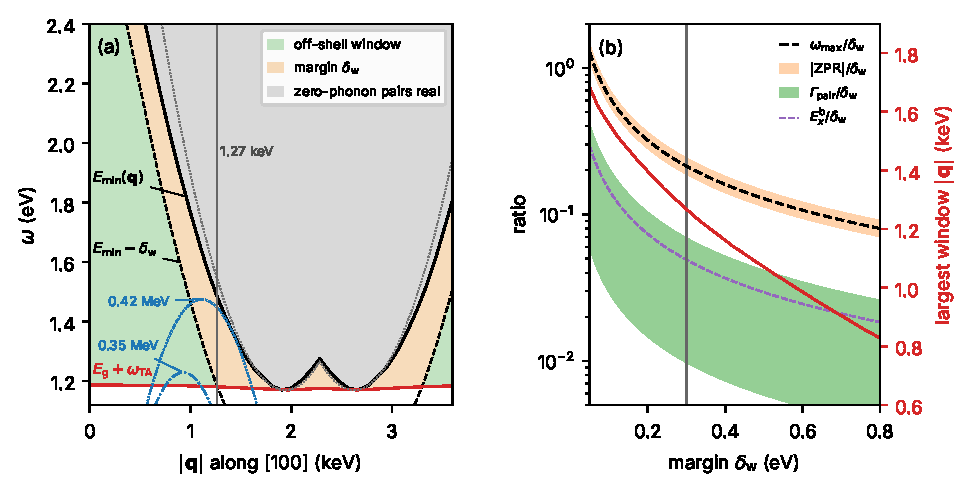
\includegraphics[width=\linewidth]{figures/ch13/fig13_6.pdf}
  \caption{The off-shell window of silicon. (a)~The plane of momentum transfer $|\vect{q}|$ along [100], the valley axis, and energy deposited $\omega$. Black: the zero-phonon edge $E_{\mathrm{min}}(\vect{q})$ from the PBE bands of \cref{fig:3-si-bands} on a $48^3$ grid, with the conduction bands shifted to the measured gap of \SI{1.17}{eV} (dotted: the parabolic valley, pair mass $1.19\,m_e$); dashed: $E_{\mathrm{min}} - \delta_{\mathrm{w}}$ with $\delta_{\mathrm{w}} = \SI{0.3}{eV}$; red: the phonon-assisted onset $\Eg + \omega_{\mathrm{TA}}(\vect{Q}^*)$ of \cref{eq:13.1-EPA}, with the PBE force constants of \cref{sec:5.2} and $\vect{Q}^*$ measured to the nearest valley, the Umklapp image of the opposite valley at \SI{2.63}{keV} included. Green: the off-shell window, where the phonon-assisted rate is a channel of its own; orange: the margin, where it is finite but its corrections grow; gray: zero-phonon pairs are real and the Dyson convention of \cref{sec:8.6} applies. Blue: the largest energy deposited by dark matter of 0.35 and \SI{0.42}{MeV}. (b)~The ratios that control the window, against the margin $\delta_{\mathrm{w}}$: top of the phonon band (\SI{64.1}{meV}), zero-point renormalization of the gap (56 to \SI{73}{meV}), width of the pair at the zero-phonon edge for $0.4 \le |\vect{q}| \le \SI{1.4}{keV}$ (3 to \SI{21}{meV}, a deformation-potential estimate with computed constants~\cite{li2021deformation}), and exciton binding energy (\SI{14.7}{meV}). Red, right axis: the largest $|\vect{q}|$ below the valley at which the window is not empty. The vertical line marks $\delta_{\mathrm{w}} = \SI{0.3}{eV}$.}
  \label{fig:13-offshell}
\end{figure}

\Cref{fig:13-offshell}(a) shows the window in the plane of $|\vect{q}|$ and $\omega$. It is a region of that plane, not an interval of $\omega$: at each $\vect{q}$ it runs from the onset $E^{\mathrm{PA}}_{\mathrm{min}}(\vect{q})$ of \cref{eq:13.1-EPA} up to $E^{\mathrm{ren}}_{\mathrm{min}}(\vect{q},T) - \delta_{\mathrm{w}}$, and it is empty where the two meet. At $|\vect{q}| = \SI{1.0}{keV}$ it spans 1.184 to \SI{1.467}{eV}. Along the valley axis it closes at $|\vect{q}| = \SI{1.27}{keV}$ with the computed bands, \SI{1.33}{keV} with the parabolic valley of \cref{sec:13.3}, and it reopens on the far side of the Umklapp image of the opposite valley, beyond \SI{3.30}{keV}. Dark matter just above the onset mass reaches only the bottom of the window. At \SI{0.42}{MeV}, where the zero-phonon line opens along this axis (\cref{sec:13.1}), the largest deposits already lie in the margin.

Between $E^{\mathrm{ren}}_{\mathrm{min}} - \delta_{\mathrm{w}}$ and $E^{\mathrm{ren}}_{\mathrm{min}}$ the amplitude is still finite, but its corrections grow as $1/(E^{\mathrm{ren}}_{\mathrm{min}} - \omega)$ and reach order one at the edge. Above the edge, within a few widths of it, no test function is smooth on the scale of the detuning, and the Dyson split of \cref{sec:8.6} has no meaning. The margin and this shell form the edge band. There we quote only totals, computed from the unexpanded amplitude \cref{eq:8.6-amp}, and no phonon-assisted rate of its own; in particular the onset exponents of \cref{eq:13.3-pon} hold only where the onset lies inside the window (\cref{sec:13.3}).

In a calculation the window is applied point by point. For each bin of $(|\vect{q}|,\hat{\vect{q}})$ the edge is the minimum of the renormalized pair energies on the full grid of $\vect{k}$, not along a symmetry line, and the bins in $\omega$ stop at that edge minus $\delta_{\mathrm{w}}$. The resonant denominators, path A with $p$ empty and path C with $p$ filled, are written as zero-phonon detunings, $\omega - E_{pv}(\vect{k},\vect{q})$ and $E_{cp}(\vect{k}+\vect{Q},\vect{q}) - \omega$, so that their smallness inside the window is visible and the energies in them are the ones that define the edge. Any smearing of the energy delta function must be small compared with $\delta_{\mathrm{w}}$, or it leaks the zero-phonon continuum into the window.

\subsection{Resonant denominators beyond the window}

Above $E^{\mathrm{ren}}_{\mathrm{min}}(\vect{q},T)$ a resonant intermediate state is a real pair. In path A it is the pair $m = (p,\vect{k}+\vect{q};\,v,\vect{k})$ with an electron in an empty band, which then emits or absorbs the phonon. In path C it is $m = (c,\vect{k}';\,p,\vect{k}+\vect{Q})$ with a hole in a filled band, which relaxes into $(v,\vect{k})$ by the phonon. Near such a state we split the amplitude into the resonant term and the rest. The resonant denominator receives the width of the pair, \cref{eq:2.4-width}:
\begin{equation}
  M^\pm_{cv\nu} = \frac{g_{fm}\,\rho_m}{\omega - \tilde E_m + \ii\varGamma_m/2} + g_{fm}\,\mathcal{A}^{\mathrm{off}}_f ,
  \label{eq:13.6-res}
\end{equation}
with $\rho_m = \rho_{pv}(\vect{k},\vect{q})$ and $g_{fm} = g_{cp\nu}(\vect{k}+\vect{q},\vect{Q})$ for path A, $\rho_m = \rho_{cp}(\vect{k}+\vect{Q},\vect{q})$ and $g_{fm} = g_{pv\nu}(\vect{k},\vect{Q})$ for path C, $\tilde E_m$ and $\varGamma_m$ the renormalized energy and the width of the pair, and $g_{fm}\mathcal{A}^{\mathrm{off}}_f$ the sum of all other terms of \cref{eq:13.2-M}; the minus sign of path C in \cref{eq:13.2-paths} is absorbed into $\rho_mg_{fm}$. A path C term has to be taken from the four-path form \cref{eq:13.2-paths}, with its many-body denominator, before the band-sum theorem is used: the width belongs to the propagator of the real pair $m$, and the theorem holds only on the energy shell (\cref{sec:13.2}). This is the amplitude \cref{eq:8.6-amp} of the level-and-band model with $\Upsilon_m$ dropped, a correction of order $g^2$.

Squared, \cref{eq:13.6-res} contains the Lorentzian $|g_{fm}\rho_m|^2/[(\omega - \tilde E_m)^2 + \varGamma_m^2/4]$, which \cref{eq:2.4-split} splits into $(2\pi/\varGamma_m)\delta(\omega - \tilde E_m)$, the finite part $\operatorname{fp}(\omega - \tilde E_m)^{-2}$ and a correction of relative order $\varGamma_m^2/\delta_{\mathrm{F}}^2$. Summed over the final states of the phonon, the delta term is $|\rho_m|^2\delta(\omega - \tilde E_m)$ times $\sum_f2\pi|g_{fm}|^2\delta(E_f - \tilde E_m)/\varGamma_m$, the fraction of the decays of $m$ that go into phonon emission. It is the zero-phonon pair, created as a real state, followed by its first decay: the cascade of \cref{sec:2.4}. The Dyson convention \cref{eq:8.6-dyson} assigns it to the zero-phonon sector with its residue, and assigns the finite part, the principal-value cross term with $\mathcal{A}^{\mathrm{off}}_f$ and $|\mathcal{A}^{\mathrm{off}}_f|^2$ to the phonon-dressed one. Outside the window, then, the phonon-assisted structure factor is $S^+$ of \cref{eq:8.6-dyson} with the substitutions above, summed over the resonances of both paths, and the zero-phonon one is $S^0$ with renormalized pairs. The two add up to the response to order $g^4$ and $\varGamma_m^2/\delta_{\mathrm{F}}^2$, against any test function smooth on the scale of the detuning $\delta_{\mathrm{F}}$ (\cref{sec:8.6}).

A computed phonon-assisted table beyond the window differs from one inside it in three ways: it need not be positive, it must not be mixed with another convention, and it is defined only near narrow lines. The finite part is negative against a narrow test function, so $S^+$ is not a positive spectrum near $\tilde E_m$, and a computed phonon-assisted table may contain negative bins near the edge; only $S^0 + S^+$ is positive. A Lorentzian zero-phonon line added to the resummed square of \cref{eq:13.6-res} counts the cascade twice, an error of order one. Added to the finite part it counts the off-shell weight twice, an error of order $g^2$ (\cref{sec:8.6}). The rate of \cref{sec:13.3} continued past the edge with a small numerical broadening in place of the width produces a delta term weighted by the inverse broadening, a cascade with an arbitrary weight.

The split is well defined only while $\varGamma_m \ll \delta_{\mathrm{F}}$, with $\delta_{\mathrm{F}}$ the distance of $\tilde E_m$ to the nearest structure of the one-phonon continuum: the zero-phonon edge itself, a threshold for emitting a further phonon, or the onset of a new valley or band. In silicon, with the widths of 3 to \SI{21}{meV} estimated above and detunings of a few tenths of an eV away from such structures, $\varGamma_m/\delta_{\mathrm{F}}$ is 0.01 to 0.1, and by \cref{eq:8.6-ambiguity} the zero-phonon weight is fixed to that order. Within a few widths of each structure it is not, and only totals are quoted, as at the edge of the window.

\subsection{The Fano term near a resonance}

When a real pair $m$ decays, the phonon it emits first interferes with the same phonon emitted directly by the off-shell paths, and \cref{eq:8.6-fano} shifts the branching of the first emission by the Fano coefficients $c^{\mathrm{F}}_\nu = \varGamma^{\mathrm{tot}}_m\Imag(\rho_m^*\mathcal{A}^{\mathrm{off}}_\nu)/|\rho_m|^2$. Their size near a resonance follows from \cref{eq:13.6-res}. With $\phi_\nu$ the phase of $\rho_m^*\mathcal{A}^{\mathrm{off}}_\nu$,
\begin{equation}
  |c^{\mathrm{F}}_\nu| = \frac{\varGamma^{\mathrm{tot}}_m}{\delta_{\mathrm{F}}}\;\frac{|\mathcal{A}^{\mathrm{off}}_\nu|\,\delta_{\mathrm{F}}}{|\rho_m|}\;|\sin\phi_\nu| .
  \label{eq:13.6-fano}
\end{equation}
The middle factor compares the off-shell amplitude with the resonant one at the distance $\delta_{\mathrm{F}}$ from the line. Both are second-order amplitudes with denominators of that size, and the factor is of order one. The Fano coefficients are therefore of first order in $\varGamma_m/\delta_{\mathrm{F}}$, the same order as the ambiguity of the Dyson split and as the branching of the cascade itself, and they need the phase $\phi_\nu$ in addition.

Symmetry controls that phase. In a crystal invariant under inversion combined with time reversal, with an even number of electrons, $(\mathsf{P}\mathsf{T})^2 = +1$ on the many-electron states, every amplitude can be made real, $\sin\phi_\nu = 0$, and the Fano term vanishes (\cref{sec:8.6}). Silicon and germanium satisfy the hypothesis at the level of one-body self-energies, with spin--orbit coupling as well: the single-electron Kramers pairs cannot all be chosen real, but the many-electron states with an even number of electrons can. If the attraction of electron and hole splits a degenerate zero-phonon manifold in a basis that is not invariant, only the sum of the coefficients over the branches vanishes. GaAs has no center of inversion, and its antisymmetric crystal potential gives $\phi_\nu$ a nonzero value. We estimate $|c^{\mathrm{F}}_\nu| \lesssim 0.3\,\varGamma_m/\delta_{\mathrm{F}}$ to first order, with the middle factor of \cref{eq:13.6-fano} set to one and $|\sin\phi_\nu| \le 0.3$ assumed for the antisymmetric part of the GaAs potential, and with Fr\"ohlich widths of a few meV just above the conduction minimum and 20 to \SI{60}{meV} higher up, $\varGamma_m/\delta_{\mathrm{F}}$ is 0.01 to 0.2 away from thresholds (\cref{app:E.14}). The Fano coefficients then move a few percent at most of the first emissions from one branch to another. Since their deviations from the mean average to zero over the branches, they change no total and no number of zero-phonon events, only which phonon the cascade starts with, and the distribution of the number of pairs by at most $\max_\nu|c^{\mathrm{F}}_\nu|$. Near each threshold $\delta_{\mathrm{F}}$ falls toward $\varGamma_m$, \cref{eq:13.6-fano} reaches order one and the expansion ends; these shells are excluded and quoted as totals. Inside the window no zero-phonon pair is real, and the Fano term does not exist.

\section{Temperature and zero-point renormalization}\label{sec:13.7}

Between room temperature and \SI{10}{mK} the indirect gap of silicon opens by \SI{46}{meV} (\cref{we:6-zpr}), and the phonon-assisted onset of \cref{we:13-onset} moves from 0.324 to \SI{0.337}{MeV}. At \SI{10}{mK} the zero-point motion still holds the gap below its clamped-nucleus value, by \SI{56}{meV} as computed at fixed volume and by 71 to \SI{73}{meV} for the electron--phonon part implied by experiment (\cref{sec:6.3}), and that renormalization is already part of the measured \SI{1.17}{eV} that every threshold of this chapter uses. It enters a detector calculation in three places. The zero-phonon response that is added to $S^{\mathrm{PA}}$ must carry it without counting anything twice, a point \cref{sec:13.3} left open. The special displacements of \cref{app:E.8}, the cheapest route to renormalized spectra, compute it together with a phonon sideband that cannot be added to the phonon-assisted rate. And the part that adiabatic methods miss must be small enough not to move the window.

\subsection{The renormalized zero-phonon response}

At order $g^2$ a zero-phonon pair is dressed in three ways: its energy is shifted, its weight is reduced, and its transition density acquires the virtual-phonon correction. All three are in the Dyson convention of \cref{sec:8.6}, which assigns to the zero-phonon sector the delta function $z_{\mathrm{qp}}(m)|\tilde\rho_m|^2\delta(\omega - \tilde E_m)$ of each pair $m$ (\cref{eq:8.6-dyson}). For a pair $(c,\vect{k}+\vect{q};\,v,\vect{k})$ the energy is the difference of the renormalized band energies \cref{eq:6.3-ren}, and the residue of the pair is, to order $g^2$, the product of the residues of electron and hole, since the slope of the pair self-energy is the sum of the slopes of $\Sigma^{\mathrm{FM}}$ for the two states (\cref{eq:4.7-qp}). The zero-phonon structure factor at temperature $T$ is then
\begin{equation}
  S^0(\vect{q},\omega;T) = 4\pi\sum_{v,c}\int_{\mathrm{BZ}}\frac{\dd^3k}{(2\pi)^3}\,
  z_{\mathrm{qp}}(c,\vect{k}+\vect{q})\,z_{\mathrm{qp}}(v,\vect{k})\,\bigl|\tilde\rho_{cv}(\vect{k},\vect{q})\bigr|^2\,
  \delta\bigl(\omega - \varepsilon^{\mathrm{ren}}_{c,\vect{k}+\vect{q}}(T) + \varepsilon^{\mathrm{ren}}_{v\vect{k}}(T)\bigr) ,
  \label{eq:13.7-S0}
\end{equation}
with $z_{\mathrm{qp}}(n,\vect{k}) = 1 + \partial_\omega\Real\Sigma^{\mathrm{FM}}_{n\vect{k}}(\omega)$ at $\omega = \varepsilon^{\mathrm{ren}}_{n\vect{k}}$, and $|\tilde\rho_{cv}|^2 = |\rho_{cv}|^2 + 2\Real(\rho_{cv}^*\,\delta\rho_{cv})$, where $\delta\rho_{cv}$ collects the mixing of bands by the off-diagonal self-energy and the virtual-phonon vertex $\Upsilon_m$ of \cref{eq:8.6-amp}. With $z_{\mathrm{qp}} = 1$, $\delta\rho = 0$ and bare energies it is \cref{eq:10.1-S0}. Temperature enters only through the phonon occupations inside the self-energies, $n_{\vect{Q}\nu} + 1 - f$ and $n_{\vect{Q}\nu} + f$ in $\Sigma^{\mathrm{FM}}$ and $2n_{\vect{Q}\nu} + 1$ in $\Sigma^{\mathrm{AH}}$ (\cref{eq:6.3-FM,eq:6.3-AH}); the band occupations are zero or one to $\ee^{-\Eg/2T}$. At \SI{1}{K} the occupation of every phonon above \SI{10}{meV} is below $10^{-50}$, and \cref{eq:13.7-S0} is the zero-point response.

The shift of the pair energies is the largest of the three corrections, and most of it is a rigid shift of the gap: in silicon the valence maximum rises by \SI{35}{meV} and the conduction minimum drops by \SI{22}{meV} (\cref{we:E-zpr}). A calculation that scissors its bands to the measured low-temperature gap has this rigid part already, and adding a computed renormalization to it counts the renormalization twice (\cref{app:E.8}). What the scissor does not supply is the variation of the shift across the zone, which \cref{sec:13.9} needs for the zero-phonon edge and which we bound below, with the nonadiabatic correction. The residues and the vertex correction change the weight of each line by an amount of relative order $\theta_{\mathrm{ep}}$ (\cref{eq:8.5-theta}), since each is one more pair of vertices on an intermediate state off the shell; in silicon near the gap $\theta_{\mathrm{ep}} = 0.010$ to 0.016 (\cref{sec:8.5}), so the weights move by one or two percent.

The weight that the zero-phonon lines lose reappears in the sideband. With all-electron (local) potentials, the electron--phonon Hamiltonian at first and second order in the displacements is a sum of one-body potentials that commute with the density. The double commutator in \cref{eq:4.3-firstmoment} is therefore that of the kinetic energy alone, $\mathscr{M}^1_{ee}(\vect{q}) = \nd_eq^2/m_e$, at every order in $g$. To order $g^2$ the electronic response with a pair in the final state is $S^0(\vect{q},\omega;T) + S^{\mathrm{PA}}(\vect{q},\omega;T)$. The density also responds without creating a pair, through the electrons dragged by the ions into a one-phonon state, and that sector has a first moment of order $g^2$ too, smaller than $\nd_eq^2/2m_e$ by about $Z_vm_e/M_{\mathrm{cell}} = 8\times10^{-5}$ in silicon. Up to that term the first moment of $S^0 + S^{\mathrm{PA}}$ equals that of the clamped-nucleus response, and
\begin{equation}
  \int_0^\infty\dd\omega\;\omega\,\bigl[S^0(\vect{q},\omega;T) - S^0(\vect{q},\omega)\bigr]
  = -\int_0^\infty\dd\omega\;\omega\,S^{\mathrm{PA}}(\vect{q},\omega;T) + O(g^4) ,
  \label{eq:13.7-fsum}
\end{equation}
where $S^0(\vect{q},\omega)$ without the temperature argument is \cref{eq:10.1-S0}, and the factor $2\pi$ and the sum over $\pm\vect{q}$ of \cref{eq:4.3-firstmoment} cancel on the two sides. The zero-phonon line gives up, in energy-weighted weight, exactly what the phonon sideband gains. The Allen--Heine term contributes nothing to this transfer: it is a static local potential, $\frac12\sum_{ab}\langle u_au_b\rangle\,\partial_a\partial_bV$, and a static local potential leaves the double commutator unchanged. The transfer is carried by the Fan--Migdal term and the vertex correction, the processes in which a phonon is emitted and reabsorbed, since $S^{\mathrm{PA}}$ is those processes with the phonon left behind. \Cref{eq:13.7-fsum} is the precise form of the overshoot of \cref{sec:13.3}, and \cref{eq:13.7-S0} removes it. Above the zero-phonon edge the bookkeeping is a percent effect on the zero-phonon rate.

\subsection{Special displacements as a quadrature}

The special displacements of \cref{app:E.8} compute renormalized spectra without vertices, from one supercell with displaced nuclei. Applied to the density response, the Williams--Lax average~\cites{lax1952franck}[Eqs.~(1) and~(3)]{zacharias2016one} is the clamped-nucleus structure factor $S^{\mathrm{cl}}(\vect{q},\omega;\{x\})$ of the supercell, averaged over the Gaussian distribution of its normal coordinates,
\begin{equation}
  S^{\mathrm{WL}}(\vect{q},\omega;T) = \prod_j\int\dd x_j\,\frac{\ee^{-x_j^2/2\sigma_j^2}}{\sqrt{2\pi}\,\sigma_j}\;S^{\mathrm{cl}}(\vect{q},\omega;\{x\}) ,
  \qquad \sigma_j^2 = \frac{2n_j + 1}{2\omega_j} ,
  \label{eq:13.7-WL}
\end{equation}
which is \cref{eq:E.8-wl} with $S$ in place of $\varepsilon_2$. Here $j = 1, 2, \ldots$ numbers the modes of the supercell, each a pair $(\vect{Q}\nu)$ of a commensurate wavevector and a branch, in order of increasing frequency, and $x_j$ are the mass-weighted coordinates $x_{\vect{Q}\nu}$ with widths $\sigma_{\vect{Q}\nu}$. The average is adiabatic by construction: each configuration is frozen while the probe acts, and the nuclei enter only through the distribution of their positions.

One configuration, with every coordinate at $x_j = \varsigma_j\sigma_j$ and signs $\varsigma_j = (-1)^{j-1}$ that alternate along the frequency-ordered list, reproduces \cref{eq:13.7-WL} as the supercell grows. Expand any smooth property $O(\{x\})$ of the frozen supercell, a band energy or $S^{\mathrm{cl}}$ at fixed $(\vect{q},\omega)$, about the equilibrium positions. The Gaussian average keeps only even powers of each coordinate,
\begin{equation*}
  \langle O\rangle_T = O(0) + \frac12\sum_j\sigma_j^2\,\frac{\partial^2O}{\partial x_j^2} + O(\sigma^4) ,
\end{equation*}
while the single configuration gives
\begin{equation*}
  O(\{\varsigma\sigma\}) = O(0) + \sum_j\varsigma_j\sigma_j\frac{\partial O}{\partial x_j} + \frac12\sum_j\sigma_j^2\frac{\partial^2O}{\partial x_j^2}
  + \frac12\sum_{j\ne k}\varsigma_j\varsigma_k\,\sigma_j\sigma_k\frac{\partial^2O}{\partial x_j\partial x_k} + O(\sigma^3) .
\end{equation*}
The diagonal second-order terms agree, because $\varsigma_j^2 = 1$. The linear terms and the cross terms must vanish. Take two neighbors in the list, $j$ and $j+1$. As the supercell grows, the commensurate grid becomes dense, the frequency spacing $\omega_{j+1} - \omega_j$ goes to zero wherever the phonon density of states is nonzero, and neighbors in the list become effectively degenerate, with the same $\sigma$. Their couplings to the electrons are not equal mode by mode, since neighbors in the list can come from distant wavevectors, but averaged over many neighbors they vary smoothly with frequency. The linear terms, which enter with alternating signs, then cancel on average, and the cross terms with any third mode $k$ cancel the same way, since $\partial_j\partial_kO$ and $\partial_{j+1}\partial_kO$ come with opposite signs~\cite[Eqs.~(6)--(9)]{zacharias2016one}. Gaps in the density of states only split the list into ranges in which the argument applies separately. What remains is the diagonal sum, which is $\langle O\rangle_T$ to order $\sigma^2$. The odd orders are removed exactly, at any supercell size, by averaging the configuration with its mirror image $x_j \to -x_j$~\cite[Eq.~(12)]{zacharias2016one}. For the higher even orders the reason is statistical: the sum $\sum_j x_j^2/\sigma_j^2$ over the Gaussian distribution has mean $N_{\mathrm{m}}$ and width $(2N_{\mathrm{m}})^{1/2}$ for $N_{\mathrm{m}}$ modes. For large supercells, as a result, almost all of the weight of \cref{eq:13.7-WL} lies on configurations with $|x_j| \approx \sigma_j$, and the special displacement is one of them~\cite[Sect.~III\,A]{zacharias2016one}. The single configuration is therefore not a random sample of the distribution but a deterministic quadrature of it, whose error falls as the grid of phonon wavevectors becomes dense.

\begin{limitbox}[Zero-point renormalization by special displacements][lim:13.7a]
$\langle\varepsilon_{n\vect{k}}\rangle_T = \varepsilon_{n\vect{k}}(\{\vect{u}^{\mathrm{ZG}}\})$ for a large supercell, with $\vect{u}^{\mathrm{ZG}}$ of \cref{eq:E.8-zg}, and to second order the adiabatic Allen--Heine--Cardona shift \cref{eq:6.3-adiabatic}~\cites{allen1981temperature}[Eqs.~(5), (10) and~(20)]{zacharias2016one}.
\par\smallskip
{\centering
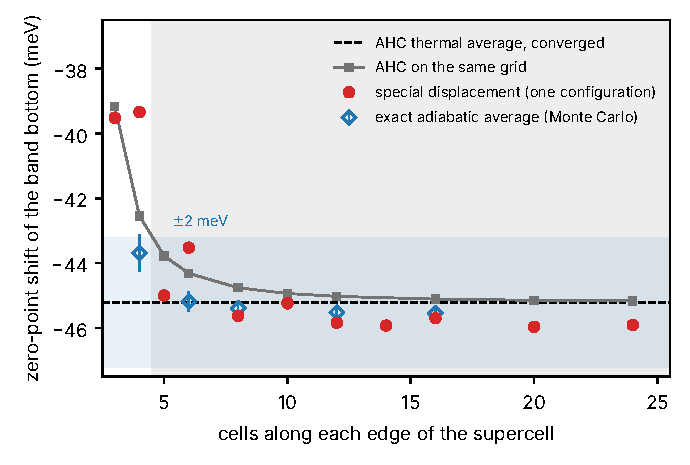
\includegraphics[width=0.92\linewidth]{figures/ch13/limit13_7a.pdf}
\captionof{figure}{Zero-point shift of the band bottom in a model crystal against the size of the supercell. The model: a simple cubic lattice, $a = \SI{2.70}{\angstrom}$, one atom of \SI{28.09}{u} per cell, central springs of 4.0 and \SI{1.5}{eV.\angstrom^{-2}} to nearest and next-nearest neighbors (phonons up to \SI{65}{meV}), and one $s$ band with nearest-neighbor hopping $t(d) = -\SI{1}{eV}\times(a/d)^6$ (band-bottom mass $0.52\,m_e$), at $T = 0$. Red: the special displacement, one configuration with every mode at its root-mean-square amplitude and signs alternating in order of frequency, wavevectors equal to their own time-reversal partners left out. Gray squares: the adiabatic Allen--Heine--Cardona average on the grid of phonon wavevectors of the same supercell; dashed: its limit for a dense grid, \SI{-45.2}{meV}, with a band of $\pm\SI{2}{meV}$. Blue diamonds: the exact adiabatic average of the same supercell, to all orders in the displacements, by Monte Carlo with antithetic pairs (statistical errors shown). Gray: supercells in which the special displacement is within \SI{2}{meV} of the limit, from $5\times5\times5$ cells (125 atoms).}\label{fig:13-zg}
\par}
\smallskip
In smaller supercells the coarse grid of phonon wavevectors and the uncancelled cross terms between modes dominate, and at any size the special displacement misses the nonadiabatic part of the renormalization and places the phonon-assisted sideband at the wrong energy.
\end{limitbox}

The model of \cref{fig:13-zg} isolates the quadrature. Its band-bottom shift is $-\SI{45.2}{meV}$ in the second-order average, $-\SI{34.5}{meV}$ from the Allen--Heine term and $-\SI{10.7}{meV}$ from the Fan term, comparable to the conduction-minimum shift of silicon. The second-order average on the grid of the supercell converges from above, and is within \SI{2}{meV} of its limit from $5\times5\times5$ cells on. The special displacement scatters around it by up to \SI{3}{meV} in the smallest supercells, where the pairing of neighbors in the frequency list is poor, and settles from $5\times5\times5$ cells on. The exact average lies \SI{0.4}{meV} below the second-order one in the larger supercells: the terms of fourth order in the displacements are one percent of the shift, and the special displacement follows the exact average rather than its second-order part, as the argument above requires. For silicon the same convergence has been computed directly: a $4\times4\times4$ supercell is within ten percent of the converged gap renormalization, and an $8\times8\times8$ supercell of 1024 atoms gives \SI{-57}{meV} (\cref{we:E-zpr}). In practice the calculation needs the phonons of the primitive cell on the commensurate grid, one density-functional calculation of the displaced supercell, and an unfolding of its bands onto the primitive zone. The convergence is checked by bracketing, with and without the self-partner wavevectors, and \cref{app:E.8} gives the procedure and its costs.

What the average contains follows from the same expansion applied to $S^{\mathrm{cl}}$. For a zero-phonon pair $f$ of the clamped crystal the energy $E_f(\{x\})$ appears inside a delta function, and the second-order term shifts it by $\frac12\sum_j\sigma_j^2\,\partial_j^2E_f$, the frozen-phonon form of \cref{eq:6.3-adiabatic}: the zero-phonon line comes out at the adiabatic Allen--Heine--Cardona energies, with a Gaussian width from the first-order terms~\cite[Eqs.~(19)--(21)]{zacharias2016one}. A pair whose crystal momentum differs from $\vect{q}$ by a phonon wavevector has no transition density in the clamped crystal, and acquires one, linear in $x_j$, in the displaced supercell. Its squared density averages to $\sigma_j^2|\partial_j\rho_f|^2$, and $\partial_j\rho_f$ is the adiabatic amplitude $M^{\mathrm{ad}}$ of \cref{eq:13.2-Mad} by \cref{eq:13.2-HT}. To second order in the displacements,
\begin{equation}
  \begin{aligned}
  S^{\mathrm{WL}}(\vect{q},\omega;T) = S^0_{\mathrm{ad}}(\vect{q},\omega;T)
  &+ \underbrace{\frac{4\pi}{\Omega}\Bigl\langle\!\Bigl\langle\sum_{\nu cv}(2n_{\vect{Q}\nu} + 1)\,\bigl|M^{\mathrm{ad}}_{cv\nu}(\vect{k},\vect{q},\vect{Q})\bigr|^2\,\delta\bigl(\varepsilon_{c,\vect{k}+\vect{q}+\vect{Q}} - \varepsilon_{v\vect{k}} - \omega\bigr)\Bigr\rangle\!\Bigr\rangle}_{S^{\mathrm{PA}}_{\mathrm{ad}}(\vect{q},\omega;T)} \\
  &+ O(\sigma^4) ,
  \end{aligned}
  \label{eq:13.7-WLexp}
\end{equation}
with $S^0_{\mathrm{ad}}$ the zero-phonon response at the adiabatic renormalized energies and the double average over $\vect{k}$ and $\vect{Q}$ as in \cref{eq:13.3-SPA}. The second term, $S^{\mathrm{PA}}_{\mathrm{ad}}$, is the adiabatic limit of $S^{\mathrm{PA}}$, the Hall--Bardeen--Blatt sideband~\cite{hall1954infrared} with the phonon energy dropped from the delta function~\cite[Eq.~(24)]{zacharias2016one}. The Williams--Lax average, and with it a special-displacement calculation, therefore contains both electronic sectors at once. Adding $S^{\mathrm{PA}}$ to it counts the sideband twice. A calculation that wants the cheap renormalized zero-phonon line and the exact sideband must subtract the adiabatic sideband computed with the same vertices, $S^{\mathrm{WL}} + S^{\mathrm{PA}} - S^{\mathrm{PA}}_{\mathrm{ad}}$, or use \cref{eq:13.7-S0} with \cref{eq:13.3-SPA} from the start.

The sideband of \cref{eq:13.7-WLexp} has the right total weight and the wrong position. Compared with \cref{eq:13.3-SPA} in the adiabatic amplitude,
\begin{equation}
  \begin{aligned}
  S^{\mathrm{PA}} - S^{\mathrm{PA}}_{\mathrm{ad}} = \frac{4\pi}{\Omega}\Bigl\langle\!\Bigl\langle\sum_{\nu cv}|M^{\mathrm{ad}}|^2\bigl[&(n + 1)\,\delta(E - \omega + \omega_{\vect{Q}\nu}) + n\,\delta(E - \omega - \omega_{\vect{Q}\nu}) \\
  &- (2n + 1)\,\delta(E - \omega)\bigr]\Bigr\rangle\!\Bigr\rangle + O\!\Bigl(\frac{\omega_{\vect{Q}\nu}}{\delta_{\mathrm{off}}}\Bigr)S^{\mathrm{PA}} ,
  \end{aligned}
  \label{eq:13.7-WLdiff}
\end{equation}
with $E = \varepsilon_{c,\vect{k}+\vect{q}+\vect{Q}} - \varepsilon_{v\vect{k}}$, $n = n_{\vect{Q}\nu}$, and the last term the amplitude error of \cref{eq:13.2-err}. The bracket integrates to zero over $\omega$, so the weights agree; its first moment is $+\sum|M^{\mathrm{ad}}|^2\omega_{\vect{Q}\nu}$, independent of temperature. At $T \gg \omega_{\vect{Q}\nu}$, or at energies far above the threshold, the three delta functions merge and the adiabatic sideband is exact. At \SI{10}{mK} it is not. There $n = 0$, the whole sideband sits at $E$ instead of $E + \omega_{\vect{Q}\nu}$, and the phonon-assisted onset falls by one phonon energy: from \SI{0.3374}{MeV} to the floor $2\Eg/v_{\mathrm{max}}^2 = \SI{0.3332}{MeV}$ (\cref{we:13-onset}). Above the onset the adiabatic spectrum is that of the exact one shifted down by $\omega_\nu$. With the onset exponent $p_{\mathrm{on}} = 3$ of \cref{eq:13.3-pon} the ratio at an energy $x$ above the true onset is $(1 + \omega_\nu/x)^3$, which falls below 1.1 only for $x > 31\,\omega_\nu$, about \SI{0.46}{eV} for the transverse acoustic phonon of the onset. At $|\vect{q}| = \SI{1}{keV}$ the whole off-shell window is \SI{0.28}{eV} wide along the valley axis and narrower off it (\cref{sec:13.6}), so nowhere inside it does the adiabatic sideband describe the rate to ten percent. Special displacements give the renormalized zero-phonon line and the spectrum far from the edges; the phonon-assisted rate in the window needs the explicit phonon energies of \cref{eq:13.3-SPA}.

\subsection{The nonadiabatic correction to the renormalization}

The adiabatic form \cref{eq:6.3-adiabatic} drops the phonon energy from the Fan--Migdal denominators. Restoring it at $T = 0$, with $\omega = \varepsilon_{n\vect{k}}$ in \cref{eq:6.3-FM}, an empty intermediate state enters only through phonon emission and an occupied one only through the absorption term with $f = 1$. The difference between the two forms is
\begin{equation}
  \mathrm{ZPR}^{\mathrm{na}}_{n\vect{k}} - \mathrm{ZPR}^{\mathrm{ad}}_{n\vect{k}} = \frac1N\sum_{\vect{Q}\nu m}|g_{mn\nu}(\vect{k},\vect{Q})|^2
  \left[\frac{1}{\varepsilon_{n\vect{k}} - \varepsilon_{m,\vect{k}+\vect{Q}} - s_m\omega_{\vect{Q}\nu}} - \frac{1}{\varepsilon_{n\vect{k}} - \varepsilon_{m,\vect{k}+\vect{Q}}}\right] ,
  \label{eq:13.7-na}
\end{equation}
with $s_m = +1$ for $m$ empty and $s_m = -1$ for $m$ occupied; the Allen--Heine term has no denominator and drops out. For an intermediate band far from $\varepsilon_{n\vect{k}}$ the bracket is smaller than the adiabatic term by $\omega_{\vect{Q}\nu}/|\varepsilon_{n\vect{k}} - \varepsilon_{m,\vect{k}+\vect{Q}}|$, a few percent for silicon. The terms that matter are those in which the intermediate state is degenerate with $(n,\vect{k})$ at $\vect{Q} = 0$: the band itself and, at the valence maximum of silicon, its partners. Take the valence maximum as a parabolic band of mass $m^*$, so that $\varepsilon_{n\vect{k}} - \varepsilon_{n,\vect{k}+\vect{Q}} = Q^2/2m^*$, coupled by an optical phonon of energy $\omega_{\mathrm{O}}$ with a vertex $g_{\mathrm{O}}$ that tends to a constant as $Q \to 0$. With $N^{-1}\sum_{\vect{Q}} = \Omega\int\dd^3Q/(2\pi)^3$ the bracket integrates in closed form,
\begin{equation}
  \begin{aligned}
  \frac{\Omega|g_{\mathrm{O}}|^2}{2\pi^2}\int_0^\infty\dd Q\,Q^2\left[\frac{1}{Q^2/2m^* + \omega_{\mathrm{O}}} - \frac{2m^*}{Q^2}\right]
  &= -\frac{\Omega|g_{\mathrm{O}}|^2}{2\pi^2}\,2m^*\int_0^\infty\frac{2m^*\omega_{\mathrm{O}}\,\dd Q}{Q^2 + 2m^*\omega_{\mathrm{O}}} \\
  &= -\frac{\Omega|g_{\mathrm{O}}|^2(2m^*)^{3/2}\sqrt{\omega_{\mathrm{O}}}}{4\pi} .
  \end{aligned}
  \label{eq:13.7-sqrt}
\end{equation}
The correction lowers the valence maximum, and with it reduces the closing of the gap. It is not of order $\omega_{\mathrm{O}}$ but of order $\sqrt{\omega_{\mathrm{O}}}$: the adiabatic integrand $2m^*/Q^2$ is integrable in three dimensions, but its weight sits at $Q \lesssim (2m^*\omega_{\mathrm{O}})^{1/2}$, exactly where the phonon energy is not small against the band dispersion. For silicon we take the optical vertex of the holes, $|g_{\mathrm{O}}| \approx \SI{0.25}{eV}$ (\cref{sec:13.6}), $\omega_{\mathrm{O}} = \SI{64.1}{meV}$, and $\Omega = a^3/4$. Three bands meet at the valence maximum without spin--orbit coupling, with the spherical masses $m_e/(\gamma^{\mathrm{Lu}}_1 \mp 2\bar\gamma^{\mathrm{Lu}}) = 0.44$ and $0.16\,m_e$ of the heavy and light holes (\cref{sec:3.3}) and $m_e/\gamma^{\mathrm{Lu}}_1 = 0.23\,m_e$ for the third. \Cref{eq:13.7-sqrt} gives 2.0, 0.4 and \SI{0.8}{meV}, together \SI{3.2}{meV}.

The full calculation finds more. Poncé and co-workers evaluated both forms of the Allen--Heine--Cardona theory for silicon in the local-density approximation on the same grids, and their indirect-gap renormalization is $-\SI{64.3}{meV}$ in the adiabatic form and $-\SI{56.2}{meV}$ in the nonadiabatic one~\cite[Table~VI]{ponce2015temperature}, the \SI{8}{meV} of \cref{sec:6.3}. Their valence maximum rises by \SI{40.9}{meV} in the adiabatic form and \SI{34.8}{meV} in the nonadiabatic one~\cite[Sect.~VI\,A\,2]{ponce2015temperature}, so \SI{6.1}{meV} of the difference sits at the valence maximum, about twice the estimate, which rests on a single vertex for all three bands. The remaining \SI{1.9}{meV} belong to the conduction minimum, which drops by \SI{23.3}{meV} in the adiabatic form and \SI{21.4}{meV} in the nonadiabatic one. Symmetry forbids an intravalley optical vertex there (\cref{sec:6.2}), and the degenerate intermediate states are the minima of the other five valleys, reached by intervalley phonons, for which the same mechanism applies. The nonadiabatic correction to the gap renormalization of silicon, defined by \cref{eq:13.7-na} as the difference between the two forms of one calculation with the same vertices and grids, is therefore \SI{8}{meV}, of which \cref{eq:13.7-sqrt} accounts for the order of magnitude and the sign, and it is precisely what special displacements miss, since they are adiabatic (\cref{lim:13.7a}). Differences between methods, such as the \SI{9}{meV} between the nonadiabatic value \SI{-56}{meV} and an adiabatic supercell value \SI{-65}{meV} compiled by Miglio and co-workers~\cite[Table~S2]{miglio2020predominance}, mix the form of the theory with the method and its inputs, and do not measure this correction.

For the window the correction does not matter, because the window is computed from the measured gap, and a measured gap contains the whole renormalization, adiabatic or not. It would enter in two ways. A calculation that builds the gap from a clamped-nucleus value, from $GW$ or a hybrid functional, plus a computed renormalization inherits the choice of form. Then \SI{8}{meV} on the gap moves the phonon-assisted onset by $\SI{0.283}{MeV.eV^{-1}}\times\SI{8}{meV} = \SI{0.0023}{MeV}$ and the zero-phonon edge by \SI{0.0015}{MeV}, with the coefficients of \cref{eq:13.7-dm} below. A calculation that scissors its bands to the measured gap misses only the variation of the renormalization between the band edges and the pair states that the zero-phonon edge reaches, about \SI{0.2}{eV} above the gap (\cref{sec:13.9}). Between the conduction minimum and the conduction state at $\mathrm{\Gamma}$, \SI{3.4}{eV} above the valence maximum, the nonadiabatic renormalization varies by \SI{14}{meV}, from $-21.4$ to $-\SI{7.4}{meV}$~\cite[Table~VI and Sect.~VI\,A\,2]{ponce2015temperature}. A variation of at most \SI{10}{meV} over the reached states is therefore a generous bound, and it moves the zero-phonon edge by at most \SI{0.002}{MeV}. Both numbers are below the spread of the computed edges themselves, 0.405 to \SI{0.408}{MeV} (\cref{sec:13.9}).

\subsection{Temperature dependence of the window}

At detector temperatures the window does not move. The measured gap $\Eg(T) = \Eg(0) - aT^2/(T + b)$ of \cref{we:6-zpr}, with $a = \SI{4.9e-4}{eV.K^{-1}}$ and $b = \SI{655}{K}$, closes by \SI{0.07}{meV} at \SI{10}{K} and by less than \SI{1}{\micro eV} at \SI{1}{K}, and the physical shift is smaller still, since the renormalization changes with the occupations $n_{\vect{Q}\nu}$, which vanish exponentially. For the transverse acoustic phonon of the onset, $n_{\mathrm{B}}(\SI{14.8}{meV})$ is $3\times10^{-8}$ at \SI{10}{K} and $2\times10^{-4}$ at \SI{20}{K}, so the emission factor $n + 1$ is one and the absorption sideband of \cref{sec:13.1} is absent below about \SI{20}{K}. The margin $\delta_{\mathrm{w}}$ of the window is measured from the renormalized edge at each temperature, and at these temperatures nothing in it depends on $T$. A detector between \SI{10}{mK} and a few kelvin sees the zero-temperature window.

At higher temperatures the gap closes, and the edges follow it. A uniform shift $\Delta\Eg(T) = \Eg(T) - \Eg(0)$ of all pair energies moves each threshold mass by the derivative of \cref{eq:13.1-mZP} or \cref{eq:13.1-mPAdef} with respect to the threshold energy, taken at the optimal momentum transfer, where the shift of the optimum itself does not contribute to first order. For a threshold $E$ reached at $q$ this derivative is $q^2/[2(qv_{\mathrm{max}} - E)^2]$, and
\begin{equation}
  \frac{\partial m_{\mathrm{min}}^{\mathrm{PA}}}{\partial\Eg} = \frac{2}{(v_{\mathrm{max}} + u_\nu)^2} = \SI{0.283}{MeV.eV^{-1}} , \qquad
  \frac{\partial m_{\mathrm{min}}^{\mathrm{ZP}}}{\partial\Eg} = \frac{2\,(m_{\mathrm{min}}^{\mathrm{ZP}})^2}{q_{\mathrm{ZP}}^2} = \SI{0.187}{MeV.eV^{-1}} .
  \label{eq:13.7-dm}
\end{equation}
For the onset we have used $q^* = 2E/(v_{\mathrm{max}} - u_\nu)$ from \cref{sec:13.1}, with the phonon energy falling as $q$ grows, $E' = -u_\nu$; the group velocity enters to first order here, although it entered the onset itself only squared, and lowers the coefficient by \SI{0.5}{\percent} from $2/v_{\mathrm{max}}^2 = \SI{0.285}{MeV.eV^{-1}}$. For the zero-phonon edge $q_{\mathrm{ZP}} = \SI{1.33}{keV}$ is the momentum transfer of the joint minimum, re-minimized on bands with spin--orbit coupling at the measured lattice constant (\cref{sec:13.9}). The zero-phonon edge moves less than the onset, because it is reached at a larger momentum transfer, where the particle has more energy to spare, and the window widens slightly as it moves down. Two effects come on top of the rigid shift. Absorption sidebands open below the onset, with the weights $n_{\mathrm{B}}(\omega_{\vect{Q}\nu})$, and the phonon energies themselves shift, but a change of one percent in $\omega_{\mathrm{TA}}(\vect{Q}^*)$ would move the onset by only $4\times10^{-5}$~MeV. At \SI{300}{K} the gap falls by $\SI{0.26}{meV.K^{-1}}$, and the onset by $7\times10^{-5}$~MeV per kelvin. \Cref{fig:13-window-T} shows the gap and the edges from \SI{10}{mK} to \SI{300}{K}.

\begin{figure}[tbp]
  \centering
  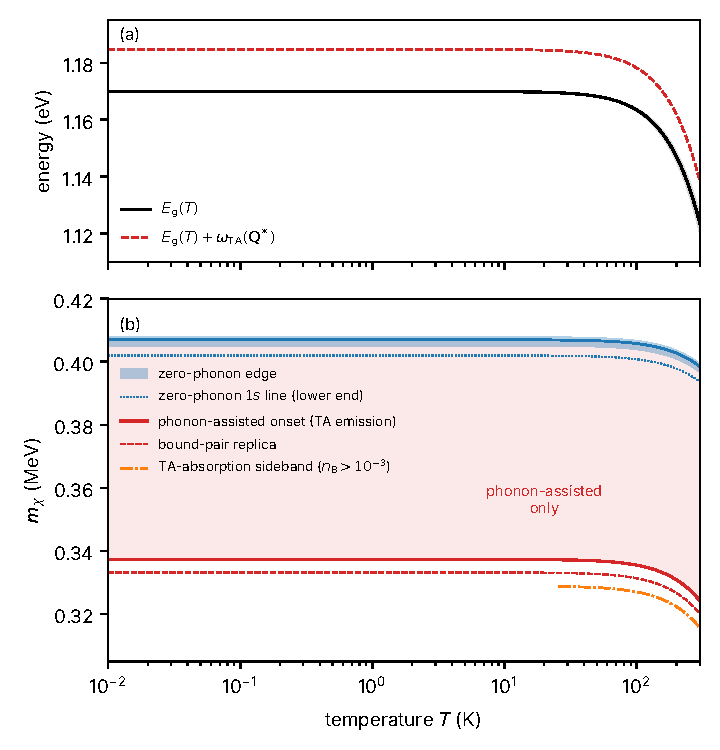
\includegraphics[width=0.8\linewidth]{figures/ch13/fig13_7.pdf}
  \caption{The silicon window against temperature, on a logarithmic temperature axis from \SI{10}{mK} to \SI{300}{K}. (a)~The indirect gap $\Eg(T) = \SI{1.17}{eV} + \Delta\Eg(T)$, with $\Delta\Eg(T)$ from the fit $\Eg(0) - aT^2/(T + b)$, $a = \SI{4.9e-4}{eV.K^{-1}}$, $b = \SI{655}{K}$, to photoluminescence data~\cites{alex1996temperature}[Eq.~(11)]{ramanathan2020ionization} (gray: $a$ and $b$ varied by their quoted errors, \SI{0.2e-4}{eV.K^{-1}} and \SI{40}{K}); dashed: the threshold of the phonon-assisted onset, $\Eg(T) + \omega_{\mathrm{TA}}(\vect{Q}^*)$. (b)~Window edges in dark-matter mass. Red: the phonon-assisted onset, transverse acoustic emission, from \cref{eq:13.1-mPAdef} with the PBE phonons of \cref{sec:5.2} and $\vect{q}$ along the valley axis; red dashed: its bound-pair replica, with $\Eg - E_x^b$, $E_x^b = \SI{14.7}{meV}$. Orange dash-dotted: the sideband with a transverse acoustic phonon absorbed, drawn where its occupation exceeds $10^{-3}$. Blue band: the zero-phonon edge, 0.405 to \SI{0.408}{MeV} at low temperature (\cref{sec:13.9}), moved with the gap at the momentum transfer of the joint minimum, \SI{1.33}{keV} (bands with spin--orbit coupling, \cref{sec:13.9}); blue dotted: the lower end of its $1s$ line. Shaded red: masses at which phonon-assisted recoil is the only electron-recoil channel. Every shift is a rigid shift of the pair energies with the measured gap.}
  \label{fig:13-window-T}
\end{figure}

\begin{workedexample}{The window shift between \SI{10}{mK} and \SI{300}{K}}\label{we:13-windowT}
\emph{Gap.} At \SI{10}{mK}, $\Delta\Eg = 0$ to $10^{-10}$~eV. At \SI{300}{K}, $\Delta\Eg = -\SI{4.9e-4}{eV.K^{-1}}\times(\SI{300}{K})^2/\SI{955}{K} = -\SI{46.2}{meV}$; with $a$ and $b$ varied by their errors, $-42.5$ to $-\SI{50.2}{meV}$.

\emph{Onset.} With $E = \Eg + \omega_{\mathrm{TA}}$ lowered by \SI{46.2}{meV}, the optimum $q^*$ falls from 0.90 to \SI{0.86}{keV}, the phonon wavevector grows from 0.46 to $0.47\,(2\pi/a)$, and the TA energy there rises from 14.78 to \SI{15.01}{meV}. Then
\begin{equation*}
  m_{\mathrm{min}}^{\mathrm{PA}}(\SI{300}{K}) = \frac{2\times(\SI{1.17}{eV} - \SI{0.0462}{eV} + \SI{0.01501}{eV})}{7.023\times10^{-6}} = \SI{0.3243}{MeV} ,
\end{equation*}
\SI{0.0131}{MeV} below the \SI{0.3374}{MeV} at \SI{10}{mK}; \cref{eq:13.7-dm} gives $\SI{0.283}{MeV.eV^{-1}}\times\SI{46.2}{meV} = \SI{0.0131}{MeV}$ directly. The bound-pair replica moves from 0.3332 to \SI{0.3201}{MeV}.

\emph{Zero-phonon edge.} At $q_{\mathrm{ZP}} = \SI{1.33}{keV}$ the edge moves by $\SI{0.187}{MeV.eV^{-1}}\times\SI{46.2}{meV} = \SI{0.0086}{MeV}$; evaluated exactly at that momentum transfer, 0.405 to \SI{0.408}{MeV} becomes 0.3966 to \SI{0.3995}{MeV}, the best value moves from 0.407 to \SI{0.3985}{MeV}, and the $1s$ line from 0.402--0.405 to 0.394--\SI{0.397}{MeV}.

\emph{Width and sidebands.} The window, from the onset to the best zero-phonon edge, spans \SI{0.0696}{MeV} at \SI{10}{mK} and \SI{0.0742}{MeV} at \SI{300}{K}. At \SI{300}{K} the absorption sidebands are open: with a TA phonon of \SI{15.2}{meV} absorbed, occupation 1.25, from \SI{0.3157}{MeV}; with an optical phonon of \SI{61.0}{meV}, occupation 0.10, from \SI{0.3027}{MeV}. At \SI{77}{K} the shifts are $-0.0011$ (onset) and $-\SI{0.0007}{MeV}$ (zero-phonon edge), and the TA absorption sideband, occupation 0.12, starts at \SI{0.3278}{MeV}.

\emph{Consequence.} A room-temperature calculation of the window, or room-temperature absorption data used for it, places both edges about \SI{0.01}{MeV} too low and adds a thermal tail that reaches \SI{0.035}{MeV} below the cold onset with one phonon absorbed, and further with several. The shift is thirty times the \SI{4e-4}{MeV} by which the softness of the computed TA branch moves the onset (\cref{we:13-onset}), and it has to be removed before a warm number describes a detector at \SI{10}{mK}.
\end{workedexample}

\section{Exciton replicas and bosonic absorption}\label{sec:13.8}

Cold silicon begins to absorb light \SI{14.7}{meV} below the free-pair threshold $\Eg(0) + \omega_{\mathrm{TA}} = \SI{1.1875}{eV}$ of \cref{sec:13.5}. The electron and the hole that a photon creates together with a transverse acoustic phonon can stay bound, by $E_x^b = \SI{14.7}{meV}$ (\cref{sec:4.9,sec:6.5}). With the measured gap $\Eg(0) = \SI{1.1692}{eV}$ of \cref{sec:6.3} the bound threshold is $\Eg(0) + \omega_{\mathrm{TA}} - E_x^b = \SI{1.1728}{eV}$. Every phonon-assisted final state of this chapter has such a bound companion. In the rate of dark-matter scattering the companions are replicas of the exciton lines, one per phonon branch, which open below the free-pair onset of \cref{sec:13.1}. For a boson that is absorbed they matter more: between the indirect gap and the direct gap at \SI{3.4}{eV} absorption needs a phonon, and at \SI{1.2}{eV} the bound pairs carry most of it.

\subsection{Exciton--phonon coupling and the replica amplitude}

The Bethe--Salpeter equation of \cref{sec:4.9} at total crystal momentum $\vect{P}$ has the eigenstates
\begin{equation*}
  |\lambda(\vect{P})\rangle = \sum_{cv\vect{k}}A^\lambda_{cv\vect{k}}(\vect{P})\,c^\dagger_{c,\vect{k}+\vect{P}}c_{v\vect{k}}\,|0\rangle ,
\end{equation*}
with the hole at $\vect{k}$, the electron at $\vect{k}+\vect{P}$, and the energies $E_\lambda(\vect{P})$. They include the bound lines and the continuum, in which each free pair is dressed by the attraction. The density creates them from the ground state with $\langle\lambda|n_e(\vect{q})|0\rangle = \sqrt{g_{\mathrm{deg}}}\,\rho_{\lambda0}(\vect{q})$, the exciton form factor \cref{eq:10.5-formfactor}. The electron--phonon Hamiltonian \cref{eq:A.6-Hep} scatters the electron or the hole of an exciton, and it creates an exciton from the ground state. With the factor $N^{-1/2}$ and the phonon matrix element taken out, as for $g_{mn\nu}$, the matrix elements between the one-pair states above are
\begin{equation}
  \begin{aligned}
  g^x_{\lambda\lambda'\nu}(\vect{q},\vect{Q}) &= \sum_{cv\vect{k}}A^{\lambda*}_{cv\vect{k}}(\vect{q}+\vect{Q})\Bigl[\sum_{c'}g_{cc'\nu}(\vect{k}+\vect{q},\vect{Q})\,A^{\lambda'}_{c'v\vect{k}}(\vect{q}) - \sum_{v'}A^{\lambda'}_{cv',\vect{k}+\vect{Q}}(\vect{q})\,g_{v'v\nu}(\vect{k},\vect{Q})\Bigr] ,\\
  g^x_{\lambda0\nu}(\vect{Q}) &= \sum_{cv\vect{k}}A^{\lambda*}_{cv\vect{k}}(\vect{Q})\,g_{cv\nu}(\vect{k},\vect{Q}) ,
  \end{aligned}
  \label{eq:13.8-gx}
\end{equation}
for an exciton $\lambda'$ at $\vect{q}$ scattered into $\lambda$ at $\vect{q}+\vect{Q}$, and for an exciton created at $\vect{Q}$. The first is the exciton--phonon vertex of Antonius and Louie~\cite[Eq.~(49)]{antonius2022theory}: the phonon vertex of the electron, or of the hole, weighted by the envelopes of the two excitons. The hole term carries the minus sign that the reordering of fermion operators gave the hole paths in \cref{sec:13.2}. The density vertex between two excitons, from $\lambda'$ at $\vect{Q}$ to $\lambda$ at $\vect{q}+\vect{Q}$, has the same structure,
\begin{equation*}
  \rho_{\lambda\lambda'}(\vect{q}) = \sum_{cv\vect{k}}A^{\lambda*}_{cv\vect{k}}(\vect{q}+\vect{Q})\Bigl[\sum_{c'}\rho_{cc'}(\vect{k}+\vect{Q},\vect{q})\,A^{\lambda'}_{c'v\vect{k}}(\vect{Q}) - \sum_{v'}A^{\lambda'}_{cv',\vect{k}+\vect{q}}(\vect{Q})\,\rho_{v'v}(\vect{k},\vect{q})\Bigr] .
\end{equation*}

The second-order amplitude \cref{eq:13.2-T} is now evaluated with exciton states. The final state holds the exciton $\lambda$ at $\vect{q}+\vect{Q}$ and one phonon more in $(-\vect{Q},\nu)$ or one fewer in $(\vect{Q},\nu)$. With the density first, the intermediate exciton $\lambda'$ sits at $\vect{q}$ and the state holds the energy $\omega$. With the phonon first, it sits at $\vect{Q}$ and the phonon has already been emitted or absorbed:
\begin{keyresult}[Exciton--phonon replica amplitude]
\begin{equation}
  \begin{gathered}
  \langle f|n_e^{(2)}(\vect{q})|i\rangle = \sqrt{\frac{g_{\mathrm{deg}}}{N}}\,\bigl(n_{\vect{Q}\nu} + \tfrac12 \pm \tfrac12\bigr)^{1/2}M^\pm_{\lambda\nu}(\vect{q},\vect{Q}) , \\
  M^\pm_{\lambda\nu}(\vect{q},\vect{Q}) = \sum_{\lambda'}\left[\frac{g^x_{\lambda\lambda'\nu}(\vect{q},\vect{Q})\,\rho_{\lambda'0}(\vect{q})}{\omega - E_{\lambda'}(\vect{q})} + \frac{\rho_{\lambda\lambda'}(\vect{q})\,g^x_{\lambda'0\nu}(\vect{Q})}{-E_{\lambda'}(\vect{Q}) \mp \omega_{\vect{Q}\nu}}\right] ,
  \end{gathered}
  \label{eq:13.8-M}
\end{equation}
on the energy shell $\omega = E_\lambda(\vect{q}+\vect{Q}) \pm \omega_{\vect{Q}\nu}$, with $\lambda'$ running over every exciton state, bound or not, of every pair of bands. The phonon-assisted structure factor with excitonic final states is
\begin{equation}
  S^{\mathrm{PA}}(\vect{q},\omega) = \frac{2\pi g_{\mathrm{deg}}}{N\Vol}\sum_{\lambda\vect{Q}\nu\pm}\bigl(n_{\vect{Q}\nu} + \tfrac12 \pm \tfrac12\bigr)\,\bigl|M^\pm_{\lambda\nu}(\vect{q},\vect{Q})\bigr|^2\,\delta\bigl(E_\lambda(\vect{q}+\vect{Q}) \pm \omega_{\vect{Q}\nu} - \omega\bigr) ,
  \label{eq:13.8-S}
\end{equation}
which replaces \cref{eq:13.3-SPA} near the edge; it does not add to it.
\end{keyresult}
\noindent The spin enters once, through the singlet exciton created by the density or by the phonon; the scattering vertices conserve it. For a bound exciton $M^\pm_{\lambda\nu}$ grows as $\Vol^{1/2}$, as $\rho_{\lambda0}$ does (\cref{sec:10.5}), and $S^{\mathrm{PA}}$ is intensive.

Without the attraction, \cref{eq:13.8-M} is the amplitude of \cref{sec:13.2}. The exciton states are then single pairs, $A^\lambda_{cv\vect{k}} = 1$ for one pair and zero otherwise, and the exciton sums become band sums. The electron term of the first part is then path A of \cref{eq:13.2-paths} and its hole term path C; in the second part the electron term is path B and the hole term path D, each with its sign and its denominator. \Cref{eq:13.8-M} is the four-path amplitude written in exciton states, and on the energy shell the band-sum theorem of \cref{sec:13.2} turns it into \cref{eq:13.2-M}. The sum over final pairs $(c,v,\vect{k})$ then carries the factor $(2\pi/\Vol)\times2\times N^{-1}\sum_{\vect{k}\vect{Q}}$, and \cref{eq:13.8-S} becomes \cref{eq:13.3-SPA}. At $\vect{q} = 0$ the form factor $\rho_{\lambda'0}$ vanishes, and in $\rho_{\lambda\lambda'}(0)$ the electron and hole terms are both $\delta_{\lambda\lambda'}$ and cancel. The amplitude vanishes, as \cref{eq:13.2-q0} requires of any phonon-assisted density amplitude.

Screening enters as in \cref{sec:13.4}. The density vertex carries the external factor $1/\varepsilon_{\mathrm{mac}}(\vect{q},\omega)$, and the exchange interaction of the final pair at its momentum contains the pair channel. What \cref{eq:13.8-M} adds is the direct kernel, the electron--hole attraction of \cref{eq:4.9-bse}, in both the intermediate and the final states. That is the excitonic part of the ladder that \cref{sec:13.4} left out.

The vertices \cref{eq:13.8-gx} need the electron--phonon vertices and the exciton envelopes in one gauge: a Bloch state enters $g$ and $A^\lambda$ with the same phase, and a phase changed in one but not the other changes $|g^x|$. In practice the vertices come from Wannier interpolation in the gauge of the interpolated bands, and the Bethe--Salpeter equation is solved on the same states. It is needed at the momenta of the silicon pockets, with about $10^3$ points of $\vect{k}$ per pocket to resolve an exciton of radius $a_x = \SI{4.2}{nm}$. For silicon and germanium that calculation is open, and a converged replica spectrum from it is the open problem of this section.

\subsection{Completeness and the two-pair test}

The sums over $\lambda'$ in \cref{eq:13.8-M} run over every one-pair state at $\vect{q}$ and at $\vect{Q}$, including the pairs whose hole lies deep in the valence band, which the hole terms of $g^x$ and $\rho_{\lambda\lambda'}$ reach. Dropping those hole terms is the exciton version of truncating the band sum to empty bands, which cost a factor of 2.4 in the model of \cref{we:13-exchange}, with the phase of its displacement wave at the cell origin. A Bethe--Salpeter basis of a few bands on each side of the gap describes the final exciton well, but not the intermediate ones, which reach every band. The $f$-sum test of the density vertices applies to the intermediate sums here as it does to \cref{eq:13.2-M}.

The space of one pair must also be the whole space of intermediate states. For independent electrons every intermediate state of \cref{eq:13.2-T} holds exactly one pair, because each vertex moves one electron (\cref{sec:13.2}). With the electron--hole interaction this is no longer exact. The Coulomb interaction contains terms that create a pair while they scatter an electron or a hole, so an exact eigenstate with one pair carries an admixture of states with two pairs, and the exact ground state an admixture of virtual pairs. \Cref{eq:13.8-M} keeps the Tamm--Dancoff space of one pair for both the intermediate and the final excitons. It is complete if the states with two pairs add nothing beyond the one-pair terms. Without interaction they do not exist, and the formula reduces to the four paths exactly. With the interaction it is unproven, and the completeness of the replica expansion reduces to the size of the two-pair sector. Its parametric estimate is the ratio of the binding energy to the gap, $E_x^b/\Eg \approx \SI{1}{\percent}$ in silicon, an estimate and not a bound.

A model with an exact two-pair sector would size this correction: a two-band chain of 8 to 12 cells with a contact attraction between electron and hole and one phonon mode, diagonalized with its states of zero, one and two pairs and compared with \cref{eq:13.8-M} built from its exact one-pair excitons.

\subsection{Replicas near the silicon edge}

Near the edge the final exciton lies within a few $E_x^b$ of the band extrema, while every intermediate exciton is far from the energy shell. By \cref{eq:13.2-doff} the distance is at least \SI{0.7}{eV} at the onset of \cref{we:13-onset}, and \SI{1.11}{eV} for absorption between the indirect and the direct gap. This separation of scales leads to a closed form. The vertices $g^x_{\lambda\lambda'\nu}$ and $\rho_{\lambda\lambda'}$ are linear in the final envelope $A^{\lambda*}(\vect{q}+\vect{Q})$, so that
\begin{equation*}
  M^\pm_{\lambda\nu}(\vect{q},\vect{Q}) = \sum_{\vect{k}}A^{\lambda*}_{cv\vect{k}}(\vect{q}+\vect{Q})\,M^{x\pm}_{cv\nu}(\vect{k},\vect{q},\vect{Q}) ,
\end{equation*}
where $M^{x\pm}$ is the amplitude into the free final pair $(c,\vect{k}+\vect{q}+\vect{Q};\,v,\vect{k})$ with exciton intermediate states. The final pair enters $M^{x\pm}$ also through the energy $\omega$ in the denominators, which moves by at most $E_x^b$ between a bound and a free final pair, a relative change $E_x^b/\delta_{\mathrm{off}}$ of about \SI{2}{\percent} at the onset and less in absorption. With free intermediate pairs, $M^{x\pm}$ is the $M^\pm$ of \cref{eq:13.2-M}. The attraction among the intermediate pairs changes it, as it changes the optical spectrum of silicon near its main peak (\cref{sec:4.9}). It does so smoothly across the zone, and changes the size of $M^{x\pm}$ at the extrema, not its variation over the small region of $\vect{k}$ that the envelope covers. With $M^{x\pm}$ held at its value $M^x_\nu$ at the extrema and $\sum_{\vect{k}}A^{\lambda*}_{\vect{k}} = \Vol^{1/2}F^*_\lambda(0)$ (\cref{sec:4.9}),
\begin{equation}
  M^\pm_{\lambda\nu}(\vect{q},\vect{Q}) \simeq \Vol^{1/2}\,F^*_\lambda(0)\,M^x_\nu ,
  \label{eq:13.8-elliott}
\end{equation}
the Elliott form \cref{eq:4.9-elliott} with the phonon-assisted amplitude in place of the density vertex~\cite{elliott1957intensity}. Only $s$ states contribute, and the shape of the edge is fixed by the final pair alone.

The final excitons are labeled by their relative motion, a bound level $n$ or a continuum state, and by their total momentum $\vect{P} = \vect{q}+\vect{Q}$, with energy $\Eg + E^{\mathrm{rel}} + (\vect{P} - \vect{k}_{\mathrm{c}})^2/2M_{\mathrm{eh}}$ near a valley by \cref{eq:4.9-dispersion}, where $M_{\mathrm{eh}}$ is the translational mass of the pair (\cref{sec:13.1}), taken isotropic. The sum over $\vect{Q}$ in \cref{eq:13.8-S} is a sum over $\vect{P}$. Insert \cref{eq:13.8-elliott} and take $T \to 0$, so that only emission survives. The factors combine as $(2\pi g_{\mathrm{deg}}/N\Vol)\,\Vol\sum_{\vect{P}} = (4\pi/N)\,N\Omega\int\dd^3\kappa/(2\pi)^3 = 4\pi\Omega\int\dd^3\kappa/(2\pi)^3$, with $\vect{\kappa} = \vect{P} - \vect{k}_{\mathrm{c}}$. The sum of $|F_\lambda(0)|^2$ over the relative states at fixed $E^{\mathrm{rel}} = E$ is the bracket of \cref{eq:10.5-lines}, which we write $\mathcal{W}_x(E)$: lines $\delta(E + E_x^b/n^2)/(\pi a_x^3n^3)$ below zero and the continuum $(2\mu_x)^{3/2}E^{1/2}F_{\mathrm{Fermi}}/4\pi^2$ above, with the Fermi factor \cref{eq:2.2-fermi} at $\xi_{\mathrm{C}} = (E_x^b/E)^{1/2}$. The integral over $\vect{\kappa}$ is the density of states of the center-of-mass motion, which the phonon leaves free. Per valley, branch and hole band,
\begin{equation*}
  S^{\mathrm{PA}}(\vect{q},\omega) \simeq 4\pi\Omega\,|M^x_\nu|^2\int\dd E\;\mathcal{W}_x(E)\,\frac{(2M_{\mathrm{eh}})^{3/2}(x - E)^{1/2}}{4\pi^2} , \qquad x = \omega - E_{\mathrm{min}}^{\mathrm{PA}}(\vect{q}) ,
\end{equation*}
with $E_{\mathrm{min}}^{\mathrm{PA}}(\vect{q})$ the free-pair threshold of \cref{eq:13.1-EPA}. Without the attraction, $\mathcal{W}_x$ is the free continuum alone, $\int_0^x\dd E\,E^{1/2}(x - E)^{1/2} = \pi x^2/8$, and the result is $\Omega(\mu_xM_{\mathrm{eh}})^{3/2}|M_\nu|^2x^2/4\pi^2$. That is \cref{eq:13.3-near}, because $\mu_xM_{\mathrm{eh}}$ is the product of the electron and hole masses for parabolic bands. Divided by this free-pair edge, the masses cancel. With $(2\mu_x)^{3/2} = 1/[a_x^3(E_x^b)^{3/2}]$ from \cref{eq:4.9-WM}, each line weight $1/(\pi a_x^3n^3)$ is $4\pi(E_x^b)^{3/2}/n^3$ in units of the continuum coefficient. Normalizing by $\pi x^2/8$ then gives the edge in closed form.
\begin{keyresult}[Replica edge in the Wannier--Mott limit]
Near the threshold of one branch, at fixed $\vect{q}$ and $T \to 0$, a phonon-assisted spectrum whose free-pair form is $A_\nu x^2$ becomes, with excitonic final states,
\begin{equation}
  A_\nu\biggl[32\,(E_x^b)^{3/2}\sum_{n\ge1}\frac{(x + E_x^b/n^2)^{1/2}}{n^3} + \frac{8}{\pi}\int_0^x\dd E\;E^{1/2}(x - E)^{1/2}\,\frac{2\pi\xi_{\mathrm{C}}}{1 - \ee^{-2\pi\xi_{\mathrm{C}}}}\biggr] ,
  \label{eq:13.8-edge}
\end{equation}
with $\xi_{\mathrm{C}} = (E_x^b/E)^{1/2}$ and each line term counted for $x > -E_x^b/n^2$. The coefficient $A_\nu$ is the one of \cref{eq:13.3-near} for dark-matter scattering and of \cref{eq:6.5-edge} for light.
\end{keyresult}
\noindent Each bound level becomes a replica edge that opens at $E_{\mathrm{min}}^{\mathrm{PA}}(\vect{q}) - E_x^b/n^2$ and rises as a square root: a line of the relative motion, spread by the center-of-mass motion. The continuum starts from zero at the free-pair threshold, but as $(32/3)(E_x^b)^{1/2}x^{3/2}$ instead of $x^2$, since the Fermi factor makes its relative-motion weight finite at the edge. These are the exponents that \cref{sec:13.3} anticipated: $\frac12$ for a replica and $\frac32$ for the excitonic continuum at fixed $\vect{q}$, and one power more each after the average over the directions of $\vect{q}$ (\cref{eq:13.3-pon}). The strength follows from the ratio of the $1s$ term to the free one at equal distance $x$ from their own thresholds, $32(E_x^b/x)^{3/2}$: 32 at $x = E_x^b$ and 5.1 at \SI{50}{meV}. The weight of the relative motion is redistributed as in \cref{sec:10.5}: the lines together hold what the free pairs hold within $8.0\,E_x^b$ of the edge, and the Fermi factor keeps the continuum above its free value far beyond.

\begin{figure}[tbp]
  \centering
  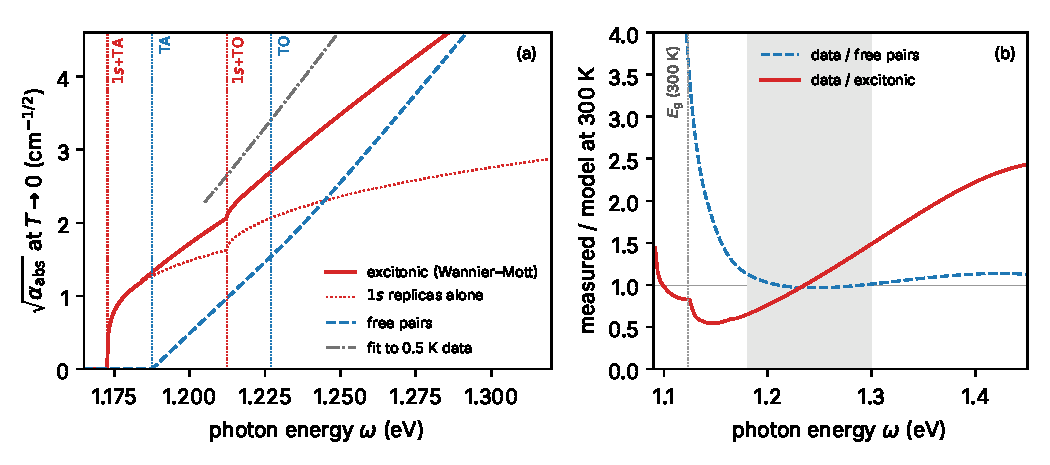
\includegraphics[width=\linewidth]{figures/ch13/fig13_8.pdf}
  \caption{Phonon-assisted absorption edge of silicon with excitonic final states. (a) $\sqrt{\alpha_{\mathrm{abs}}}$ at $T \to 0$ against the photon energy. Red: \cref{eq:13.8-edge} for the transverse acoustic and transverse optical branches, $\omega_{\mathrm{TA}} = \SI{18.27}{meV}$ and $\omega_{\mathrm{TO}} = \SI{57.73}{meV}$, with weights $5.5:4.0$~\cite{rajkanan1979absorption,stanford2021photoelectric}, $\Eg(0) = \SI{1.1692}{eV}$ and $E_x^b = \SI{14.7}{meV}$ for both hole bands; dotted, the two $1s$ replicas alone. Blue, dashed: the free-pair edge of \cref{sec:13.5}. Each model has one scale, fitted as in \cref{sec:13.5} to the measured \SI{300}{K} absorption between 1.18 and \SI{1.30}{eV}~\cite{franta2017temperature}. Gray, dash-dotted: the free-pair form fitted to measurements between 0.5 and \SI{295}{K}, with an effective gap of \SI{1.134}{eV}, evaluated at \SI{0.5}{K} and drawn above \SI{1.205}{eV}, the lowest photon energy measured~\cite[Eqs.~(4)--(7)]{stanford2021photoelectric}. Vertical lines: the $1s$ replica thresholds $\Eg - E_x^b + \omega_\nu$ (red) and the free-pair thresholds $\Eg + \omega_\nu$ (blue). (b) Measured absorption at \SI{300}{K} divided by each model at \SI{300}{K}, both branches with their phonon occupations; gray band, the fitted interval. Effective-mass models with constant matrix elements, not calculations.}
  \label{fig:13-replicas}
\end{figure}

\Cref{fig:13-replicas}a shows \cref{eq:13.8-edge} for cold silicon. The $1s$ replica of the transverse acoustic branch opens at \SI{1.1728}{eV} and the $2s$ replica at \SI{1.1838}{eV}, both below the free-pair threshold at \SI{1.1875}{eV}; the transverse optical replica opens at \SI{1.2122}{eV}. With the same $|M^x_\nu|^2$ the excitonic edge of the two branches exceeds the free-pair one by a factor of 81 at \SI{1.200}{eV}, 16 at \SI{50}{meV} above the free threshold and 7.3 at \SI{100}{meV}, and at \SI{1.200}{eV} the $1s$ replica holds three quarters of it.

The measured spectra test the shape. Fitted in the same interval of the \SI{300}{K} data, the excitonic form needs a scale 0.154 times that of the free-pair form, since the Fermi factor already supplies part of the absorption there. Neither form follows the data over the whole range (\cref{fig:13-replicas}b). The free-pair form falls short within \SI{40}{meV} of the gap, by the factor 2.0 at \SI{17}{meV} found in \cref{sec:13.5}. The hydrogenic form overshoots there by up to 1.8 and falls short by 1.5 to 2.5 between 1.3 and \SI{1.6}{eV}, where the parabolic bands and the hydrogenic continuum of \cref{sec:10.5} no longer hold. The edge region is where the excitonic form belongs, and there the measurements at low temperature are the test. At \SI{1.21}{eV}, the lowest energy measured at \SI{0.5}{K}, the fit to the measurements, evaluated at that temperature, is \SI{6.4}{cm^{-1}}, the excitonic form 4.0 and the free-pair form \SI{0.77}{cm^{-1}}. With the decrease of the branch strength between the lowest temperature and \SI{295}{K} found in \cref{sec:13.5}, a factor 0.61, the excitonic value becomes 6.6 and the free-pair one 1.3. The fit itself needs an effective gap of \SI{1.134}{eV}, \SI{35}{meV} below the true one: a free-pair form can follow an excitonic edge only by moving its threshold down.

For dark-matter scattering the same construction applies at each $\vect{q}$, with $A_\nu$ the coefficient of \cref{eq:13.3-near} and the thresholds $E_{\mathrm{min}}^{\mathrm{PA}}(\vect{q}) - E_x^b/n^2$. The binding energy is that of the pair at the momentum $\vect{q}+\vect{Q}^*$, near $\vect{k}_{\mathrm{c}}$, where the hole sits near the valence maximum and the measured \SI{14.7}{meV} applies; its variation along the dispersion of the pair is \cref{eq:E.15-disp}. The lightest mass at which the $1s$ replica opens follows from \cref{eq:13.1-mPA} with $\Eg$ replaced by $\Eg - E_x^b$, as \cref{sec:13.1} found, and its value and status belong to \cref{sec:13.9}.

\subsection{Phonon-assisted absorption of bosonic dark matter}

Absorption of a boson probes the response at $\vect{q} = \vect{p}_\phi$, about $10^{-3}m_\phi$, and $\omega = m_\phi$ (\cref{eq:8.2-abs}). In silicon between the excitonic edge at \SI{1.1728}{eV} and the direct gap $E_{\mathrm{dir}} = \SI{3.4}{eV}$ no vertical pair exists. Every first-order transition at $\vect{q} \simeq 0$ is then off the energy shell, and the window of \cref{eq:13.6-window}, with the vertical gap as the zero-phonon edge, extends to $E_{\mathrm{dir}} - \delta_{\mathrm{w}} = \SI{3.1}{eV}$. Inside it every response row is phonon-assisted. Its structure factor is \cref{eq:13.3-SPA} at $\vect{q} = 0$ with the vertices of the two rows in place of $\rho$, or \cref{eq:13.8-S} near the edge. Each of the three rates of \cref{sec:10.7} therefore holds there with its response replaced by the phonon-assisted one. The bosons differ in whether that response is measured.

The dark photon has no phonon-assisted amplitude of its own at first order in $g$. It couples to the electromagnetic current of electrons and nuclei with $\zeta$ times the charge of the photon, and every second-order amplitude into a pair and one phonon reduces to that of light or vanishes. The electron current with one electron--phonon vertex is the amplitude of light, \cref{eq:6.5-M} with the velocity vertex, and its square summed over final states is the measured $\varepsilon_2^{\mathrm{PA}}$. The longitudinal polarization couples to the charge density at $\vect{q} = \vect{p}_\phi$, and the phonon-assisted density amplitude there is, by continuity, $(q/\omega)$ times the velocity amplitude (\cref{eq:13.5-Mlim}). It is the same amplitude written another way, and adding the density form of \cref{sec:13.2} to the current form would count the transition twice. The nuclear current, finally, changes a phonon occupation at $\vect{Q} \simeq \vect{p}_\phi$ without moving an electron, while the electron--phonon vertex moves one electron and changes one occupation. Together they either leave two occupations changed, a final state with two phonons, or remove the phonon the current created and leave a vertical pair, which needs $\omega \ge E_{\mathrm{dir}}$; in silicon the Born charges vanish in any case. The rate is \cref{eq:10.7-dp} with $L = \varepsilon_2^{\mathrm{PA}}/(\varepsilon_1^0)^2$ at the temperature of the detector (\cref{sec:13.4,sec:13.5}). At the edge $\varepsilon_2^{\mathrm{PA}}$ is of order $10^{-4}$, so the phonon-assisted part of the photon self-energy does nothing to the mixing, and $\zeta_{\mathrm{eff}} = \zeta/\varepsilon_1^0$. What the dark photon needs is the measured edge itself, brought to millikelvin temperatures and resolved into its excitonic structure, as \cref{we:13-darkphoton-edge} shows.

The axion-like particle couples through the spin current $\mathcal{J}_e$ (\cref{sec:10.7-alp}). The electron--phonon vertex is diagonal in spin. The spin structure of the phonon-assisted amplitude is therefore that of the one spin operator in $\mathcal{J}_e$, and the spin trace of \cref{sec:10.7-alp} goes through unchanged: $S^{\mathrm{PA}}_{\mathcal{J}\mathcal{J}} = \frac34S^{\mathrm{PA}}_{jj}$ and $\varGamma = (3m_\phi^2/4m_e^2)(g_{aee}^2/e^2)\,\sigma_1^{\mathrm{PA}}$, with $\sigma_1^{\mathrm{PA}} = m_\phi\varepsilon_2^{\mathrm{PA}}$, for independent electrons without spin--orbit coupling. At equal couplings it is $(3m_\phi^2/4m_e^2e^2)|\varepsilon|^2 = 7.3\times10^{-9}$ of the dark-photon rate at \SI{1.2}{eV}. The caveats of \cref{sec:10.7-alp} take a specific form at the edge. The spin current creates triplet pairs, which feel the direct kernel and not the exchange one (\cref{eq:10.5-triplet}). The replica lines are therefore the same as in the measured singlet edge, up to the exchange splitting, which is about $2\times10^{-3}$ of the binding (\cref{sec:10.5}). The pair channel of \cref{sec:13.4}, a Coulomb screening at the pair momentum, is absent from the triplet response, and its size is not known for the singlet either.

The scalar couples through two rows, the density and the kinetic energy (\cref{sec:10.7-scalar}). The phonon-assisted density amplitude vanishes at $\vect{q} = 0$ by \cref{eq:13.2-q0}, so the density row enters at order $p_\phi$ and its rate at order $v^2$. The kinetic row, however, does not vanish. Its phonon-assisted amplitude $M^\pm_{\mathcal{T},cv\nu}(\vect{k},\vect{Q})$ is \cref{eq:13.2-M} at $\vect{q} = 0$ with the vertical kinetic elements $(\mathcal{T}_e)_{mn}(\vect{k}) = \langle m\vect{k}|p^2/2m_e|n\vect{k}\rangle$ in place of $\rho_{mn}$, and its intraband terms no longer cancel. Path A with $p = v$ and path B with $p = c$ add to $g_{cv\nu}(\vect{k},\vect{Q})[(\mathcal{T}_e)_{vv}(\vect{k}) - (\mathcal{T}_e)_{cc}(\vect{k}+\vect{Q})]/\omega$, the difference of the kinetic energies of the two band states, where the density has $\rho_{vv} = \rho_{cc} = 1$. The whole amplitude has a compact form. In the operator form of \cref{eq:13.2-M} (\cref{app:D.35}), $\langle c|y\,(\varepsilon_v + \omega - h)^{-1}x + x\,(\varepsilon_v \mp \omega_{\vect{Q}\nu} - h)^{-1}y|v\rangle$ with $x = p^2/2m_e$ and $y$ the phonon vertex, write $x = h - V$, with $h$ the one-electron Hamiltonian and $V$ everything in it but the kinetic energy. The part $h$ acts on $|v\rangle$ in the first term and on $\langle c|$ in the second, where it returns $\varepsilon_v$ and $\varepsilon_c$, and the resolvents return $1/\omega$ and $-1/\omega$ on the shell. With $\varepsilon_c - \varepsilon_v = \omega \mp \omega_{\vect{Q}\nu}$,
\begin{equation}
  M^\pm_{\mathcal{T},cv\nu}(\vect{k},\vect{Q}) = -\Bigl(1 \mp \frac{\omega_{\vect{Q}\nu}}{\omega}\Bigr)\,g_{cv\nu}(\vect{k},\vect{Q}) - M^\pm_{V,cv\nu}(\vect{k},\vect{Q}) ,
  \label{eq:13.8-MT}
\end{equation}
where $M^\pm_V$ is \cref{eq:13.2-M} at $\vect{q} = 0$ with the matrix elements of $V$ in place of $\rho$. The first term is the electron--phonon vertex itself. The second is the phonon-assisted amplitude of the crystal potential, the counterpart of $\langle c|p^2/2m_e|v\rangle = -\langle c|V|v\rangle$ of \cref{sec:10.7-scalar}, and like it weighted toward the cores. Both are of order $g$ in energy units, and nothing cancels them. \Cref{eq:10.7-scalar} with the phonon-assisted response is
\begin{equation}
  \begin{gathered}
  \varGamma = \frac{g_{\phi ee}^2}{2\,m_\phi m_e^2}\,S^{\mathrm{PA}}_{\mathcal{T}\mathcal{T}}(0,m_\phi) , \\
  S^{\mathrm{PA}}_{\mathcal{T}\mathcal{T}}(0,\omega) = \frac{4\pi}{\Omega}\Bigl\langle\!\Bigl\langle\sum_{\nu cv\pm}\bigl(n_{\vect{Q}\nu} + \tfrac12 \pm \tfrac12\bigr)\bigl|M^\pm_{\mathcal{T},cv\nu}\bigr|^2\delta\bigl(\varepsilon_{c,\vect{k}+\vect{Q}} - \varepsilon_{v\vect{k}} \pm \omega_{\vect{Q}\nu} - \omega\bigr)\Bigr\rangle\!\Bigr\rangle ,
  \end{gathered}
  \label{eq:13.8-scalar}
\end{equation}
unscreened, for a point group without a polar vector, inside the window; near the edge the final pairs are the excitons of \cref{eq:13.8-S} with the kinetic row in place of the density. No measurement provides this response, and it is not proportional to $\varepsilon_2^{\mathrm{PA}}$, since \cref{eq:13.8-MT} has no velocity vertex in it. The comparison with the axion-like particle in \cref{sec:10.7-scalar} carries over. The kinetic amplitude is of the order of the vertex $g$, while the axion-like amplitude carries $m_\phi/m_e$ times an electron velocity. At equal couplings the scalar is therefore absorbed far more strongly, by a factor that only a calculation fixes. The phonon-assisted kinetic absorption has been computed for the intraband transitions of a superconducting metal~\cite[Sect.~V, Eq.~(72)]{mitridate2021dark}; a silicon rate built from vertical transitions has below about \SI{3}{eV} only the tails of the smearing~\cite[Sect.~IV]{mitridate2021dark}. The interband channel of \cref{eq:13.8-MT,eq:13.8-scalar} at the indirect edge of an insulator needs, for its evaluation, a phonon-assisted kinetic row with all-electron kinetic matrix elements.

\begin{workedexample}{A dark photon of 1.2 eV in cold silicon}\label{we:13-darkphoton-edge}
At $m_\phi = \SI{1.200}{eV}$ a dark photon sits \SI{12.5}{meV} above the free-pair threshold $\Eg(0) + \omega_{\mathrm{TA}} = \SI{1.1875}{eV}$ and \SI{27.2}{meV} above the $1s$ replica, below both transverse optical thresholds. Only the transverse acoustic branch absorbs, by emission.

\emph{Cold absorption.} Stanford and co-workers fitted their data at 0.5 to \SI{295}{K} with the free-pair form $\alpha_{\mathrm{abs}} = \sum_\nu C_\nu c_0(\omega - E_{\mathrm{g}1} - \omega_\nu)^2$ at low temperature, with the branch weights $C_{\mathrm{TA}} = 5.5$ and $C_{\mathrm{TO}} = 4.0$, the strength $c_0 = \SI{325}{eV^{-2}.cm^{-1}}$ and an effective gap $E_{\mathrm{g}1} = \SI{1.134}{eV}$~\cite[Eqs.~(4)--(7)]{stanford2021photoelectric}. Evaluated at \SI{0.5}{K}, it gives $\alpha_{\mathrm{abs}} = 5.5\times\SI{325}{eV^{-2}.cm^{-1}}\times(\SI{0.0477}{eV})^2 = \SI{4.07}{cm^{-1}}$ from its transverse acoustic term and \SI{0.09}{cm^{-1}} from the transverse optical one, which its lowered gap opens: \SI{4.16}{cm^{-1}}, \SI{6}{meV} below their lowest photon energy. The \SI{20}{K} data of Macfarlane and co-workers~\cite{macfarlane1958fine} give \SI{0.21}{cm^{-1}} at this energy, twenty times less; near the edge the cold datasets differ by that much (\cref{sec:13.9-rates}). The excitonic edge of \cref{fig:13-replicas} reaches \SI{2.95}{cm^{-1}} (4.8 with the strength factor 0.61), the free-pair edge transferred to millikelvin temperatures in \cref{sec:13.5} only \SI{0.24}{cm^{-1}}, and the \SI{300}{K} data used without transfer \SI{27.3}{cm^{-1}}.

\emph{Loss function.} With the fit value $\alpha_{\mathrm{abs}} = \SI{4.16}{cm^{-1}}$, $n_r = 3.565$ from the \SI{300}{K} data and $\hbar c/\omega = \SI{1.644e-5}{cm}$,
\begin{equation*}
  \varepsilon_2^{\mathrm{PA}} = n_r\,\alpha_{\mathrm{abs}}\,\frac{\hbar c}{\omega} = 2.44\times10^{-4} , \qquad
  L = \frac{\varepsilon_2^{\mathrm{PA}}}{(\varepsilon_1^0)^2} = \frac{2.44\times10^{-4}}{12.71^2} = 1.51\times10^{-6} .
\end{equation*}
The medium suppresses the rate by $|\varepsilon|^2 = 161.5$ against the vacuum mixing.

\emph{Rate.} With $\rho_\chi = \SI{0.3}{GeV.cm^{-3}}$ and $\rho_T = \SI{2.33}{g.cm^{-3}}$, $(\rho_\chi/\rho_T)/\hbar = 6.17\times10^{33}$ per kilogram-year, as in \cref{we:10-darkphoton}, and \cref{eq:10.7-dp} gives
\begin{equation*}
  \mathcal{R} = 6.17\times10^{33}\times1.51\times10^{-6}\,\zeta^2 = 9.3\times10^{27}\,\zeta^2\ \text{per kilogram-year} .
\end{equation*}
Three events in a kilogram-year need $\zeta = 1.8\times10^{-14}$. The untransferred \SI{300}{K} data would claim a rate 6.6 times larger and $\zeta = 7.0\times10^{-15}$; the transferred free-pair edge a rate 17 times smaller and $\zeta = 7.5\times10^{-14}$, and the \SI{20}{K} data a rate 20 times smaller. At \SI{1.2}{eV} the correction that matters is the bound pair: in the excitonic edge three quarters of the absorption at this energy is the $1s$ replica, which neither the warm data nor the free-pair transfer represents.
\end{workedexample}

\section{The silicon window}\label{sec:13.9}

A silicon detector that counts single electrons sees dark matter of \SI{0.36}{MeV} only through the phonon-assisted rate, and dark matter of \SI{0.6}{MeV} almost only through zero-phonon pairs. Kinematics fixed the onset of the first at 0.3332 and \SI{0.3374}{MeV} and put upper values on the second along chosen directions (\cref{sec:13.1}). Here the zero-phonon side is evaluated with bands over the whole zone: the first zero-phonon edge lies at 0.405 to \SI{0.408}{MeV}, off the valley axis, and its state is weakly coupled because a glide of the diamond structure forbids its vertex. These edges and their order rest on two independent calculations. Where the phonon-assisted rate stops leading, how large it is, and the windows of germanium and GaAs are known only as estimates or not at all.

\subsection{The zero-phonon edges}\label{sec:13.9-edges}

The joint minimum \cref{eq:13.1-mZP} over the momentum transfer and the hole's crystal momentum lies off the valley axis. The search uses the PBE bands of \cref{sec:3.4}, interpolated in Wannier functions, with the conduction bands shifted rigidly to the measured gap $\Eg(0) = \SI{1.170}{eV}$. Of 21 starting points, 18 converge on one point up to the cubic symmetry, and a local re-minimization on the plane-wave bands at the measured lattice constant refines it. The optimum has $|\vect{q}| = \SI{1.33}{keV}$, tilted by \SI{0.18}{rad} from the [100] axis within a $\{001\}$ plane. The hole sits at $\vect{k}_v = (0.126, -0.107, 0)\,(2\pi/a)$, \SI{62}{meV} below the valence-band maximum, along a direction in which the heavy-hole band is flat (its PBE mass along [110] is about $2.5\,m_e$). The electron sits on the valley axis, about $0.16\,(2\pi/a)$ short of the valley minimum. The pair costs \SI{1.355}{eV}, and the threshold mass is
\begin{equation*}
  m_{\mathrm{min}}^{\mathrm{ZP}} = \SI{0.407}{MeV} ,
\end{equation*}
with spin--orbit coupling, and \SI{0.404}{MeV} without, within a band of 0.405 to \SI{0.408}{MeV} that carries the lattice constant and the interpolation. The $1s$ exciton lowers it by $\mchi E_x^b/(qv_{\mathrm{max}} - E) = \SI{0.0028}{MeV}$ (\cref{sec:13.1}), to 0.402--\SI{0.405}{MeV}.

The joint minimum leaves the axis because, at $|\vect{q}| = 1.2$ to \SI{1.48}{keV}, the [100] axis is a local maximum of $E_{\mathrm{min}}(\vect{q})$ over the directions of $\vect{q}$, not a minimum. The minima sit 0.13 to \SI{0.22}{rad} away in the $\{001\}$ planes, 14 to \SI{107}{meV} below the on-axis value, and are shallower in the $\{011\}$ planes. Around the optimum the pair energy rises as $\beta_\theta\vartheta^2 + \beta_z\varphi^2$, with $\beta_\theta = \SI{2.47}{eV.rad^{-2}}$ for the tilt within the plane and $\beta_z = \SI{3.70}{eV.rad^{-2}}$ out of it. The warped heavy hole of \cref{eq:3.3-holes} is the cause: moving the hole into its flat direction costs less than the pair kinetic energy it saves. On the axis the same bands have a local optimum at \SI{0.415}{MeV}, which the coarser grid of \cref{sec:13.1} placed at \SI{0.420}{MeV} and the parabola at \SI{0.425}{MeV}. The joint minimum is therefore 0.013 to \SI{0.018}{MeV} below the upper values of \cref{sec:13.1}.

Spin--orbit coupling raises the edge by \SI{0.003}{MeV}, fifteen times more than on the axis. At the optimum the hole lies \SI{62}{meV} below the valence maximum, deeper than the split-off energy ($\Delta_{\mathrm{SO}} = \SI{48.6}{meV}$ in PBE, \SI{44}{meV} measured, \cref{tab:3-materials}), and it does not share the rise by $\Delta_{\mathrm{SO}}/3$ of the $\mathrm{\Gamma}_8$ maximum to which the gap is referred. With spin--orbit coupling it sits \SI{77}{meV} below that maximum, and the pair costs \SI{15.5}{meV} more. On the axis, where the hole is near $\mathrm{\Gamma}$, the shift is under \SI{1}{meV}.

Three further edges complete the zero-phonon side. On the axis the two heavy holes are degenerate. A tilt within a $\{001\}$ plane splits them into one band that is odd under the mirror of that plane and one that is even, and they open at different masses. The first edge belongs to the odd band. The even band reaches the same pair energy only on the axis, and its edge lies at 0.415 to \SI{0.420}{MeV}, the range set by the lattice constant and spin--orbit coupling. Off the axis its pair energy rises as $\beta_2\vartheta^2$, with $\beta_2$ from \SI{4.5}{eV.rad^{-2}} in the $\{001\}$ planes to \SI{1.1}{eV.rad^{-2}} in the $\{011\}$ planes. The third edge is that of the Umklapp class $\vect{G}' = (\bar2\,0\,0)\,2\pi/a$, in which the unreduced crystal momentum of the electron lies beyond the X face of the zone, so that the reciprocal-lattice vector sits inside the density vertex (\cref{sec:3.1}). Restricted to this class, \cref{eq:13.1-mZP} has its minimum on the X face, at $|\vect{q}| = \SI{1.83}{keV}$ with the hole at $|\vect{k}_v| = 0.26\,(2\pi/a)$: the line opens at \SI{0.50}{MeV}, spin--orbit coupling included. The last edge of the class without Umklapp on the [100] axis is far above all of these. Along [110] and [111], 0.548 and \SI{0.615}{MeV} (\cref{sec:13.1}), the zero-phonon channel is already open through the other edges.

The edges fall in a fixed order:
\begin{equation*}
  \underbrace{0.3332 < 0.3374}_{\text{phonon-assisted onset}}
  < \underbrace{0.402\text{--}0.405 < 0.405\text{--}0.408}_{\text{first zero-phonon edge}}
  < \underbrace{0.415\text{--}0.420}_{\text{second heavy hole}}
  < \underbrace{\approx 0.50}_{(\bar2\,0\,0)\ \text{line}}\ \si{MeV} .
\end{equation*}
The order does not depend on the last digits. The phonon-assisted onset moves by \SI{2.8e-4}{MeV} per meV of phonon energy (\cref{we:13-onset}), and even a transverse acoustic phonon at its largest energy, \SI{18.6}{meV} at X, would put it at \SI{0.339}{MeV}, \SI{0.07}{MeV} below the first zero-phonon edge. The zero-phonon edges are separated by more than their own spreads. Between the onset and the first edge no zero-phonon pair exists at any momentum transfer, and the phonon-assisted rate is the only electron-recoil channel; above the first edge the question becomes one of rates.

These are thresholds, not rates, and they are cheap. The joint minimization needs interpolated bands over the zone with a gap correction, a check of the interpolated pair energy against a direct plane-wave calculation at the optimum (it differs by \SI{11}{meV}), and a local re-minimization with spin--orbit coupling (\cref{app:E.1}). \Cref{app:E.14} specifies the bins on which the zero-phonon rate is to be computed next to the phonon-assisted one: the cones around the mirror-plane optima, the cone of the second heavy hole and the X-face edge.

\subsection{The glide-parity selection rule}\label{sec:13.9-glide}

On the valley axis, without Umklapp, the zero-phonon vertex between the bottom of the valley and the valence maximum vanishes. The electron is invariant under the operations that fix the axis, and the holes have no invariant part (\cref{sec:10.5-rules}; in the language of \cref{sec:13.3}, $\Delta_1\otimes\Delta_1\otimes(\Delta_2'\oplus\Delta_5)$ contains no $\Delta_1$). Off the axis these operations are gone, and only one survives for a pair that stays in a $\{001\}$ plane through the axis: the mirror of that plane. In diamond it carries the fractional translation $\vect{\tau}_2$ and is a glide (\cref{app:C.17}). Bloch states with crystal momentum in the plane are its eigenstates, with a glide parity $\eta = \pm1$ (\cref{eq:C.17-parity}). The density vertex with $\vect{q}$ in the plane connects a valence state of parity $\eta_v$ to the conduction state of reduced parity $\eta_c$ only if
\begin{equation}
  \eta_c\,\eta_v\,\ee^{-\ii\vect{G}'\cdot\vect{w}/2} = 1 ,
  \label{eq:13.9-glide}
\end{equation}
where $\vect{G}'$ is the Umklapp vector of the unreduced final momentum and $\vect{w}$ the lattice vector that the glide gives when applied twice. This is \cref{eq:C.17-selection} applied to the mirror $\mathsf{m}_z$. The rule decides which zero-phonon line is strong at each of the edges.

\begin{workedexample}{The selection rule for the first zero-phonon line}\label{we:13-glide}
Take the valley on the $x$ axis and the mirror $\mathsf{m}_z$, $(x, y, z) \to (x, y, -z)$, whose plane $z = 0$ contains the axis and the optimum of \cref{sec:13.9-edges}. In diamond it occurs as $g = \{\mathsf{m}_z|\vect{\tau}_2\}$ with $\vect{\tau}_2 = (a/4)(1,1,1)$, as in \cref{eq:C.17-glide} with $x$ and $z$ exchanged. Applied twice it gives the translation $\vect{w} = \vect{\tau}_2 + \mathsf{m}_z\vect{\tau}_2 = (a/2)(1,1,0)$, a lattice vector.

\emph{The phase of the operator.} Conjugating the vertex gives $g\,\ee^{\ii\vect{q}\cdot\vect{r}}g^{-1} = \ee^{-\ii\vect{q}\cdot\vect{\tau}_2}\ee^{\ii\vect{q}\cdot\vect{r}}$ for $\vect{q}$ in the plane. Against the phases $\ee^{-\ii\vect{k}\cdot\vect{w}/2}$ of the two eigenvalues it leaves $\ee^{\ii\vect{q}\cdot(\vect{w}/2 - \vect{\tau}_2)}$, and $\vect{w}/2 - \vect{\tau}_2 = (0, 0, -a/4)$ is normal to the plane, so this phase is one. With unreduced labels the vertex therefore needs $\eta_c = \eta_v$.

\emph{Reduced labels.} Reducing the final momentum by $\vect{G}'$ multiplies the conduction eigenvalue by $\ee^{-\ii\vect{G}'\cdot\vect{w}/2}$. For $\vect{G}' = 0$ the factor is one and \cref{eq:13.9-glide} requires equal parities. For $\vect{G}' = (\bar2\,0\,0)\,2\pi/a$, $\vect{G}'\cdot\vect{w}/2 = -(4\pi/a)(a/4) = -\pi$, the factor is $-1$, and the parities must be opposite. Every vector of the (200) class flips the rule; vectors with $h + k \equiv 0 \pmod 4$ in the plane keep it.

\emph{On the axis.} The heavy-hole pair $\Delta_5$ splits under the mirror into one even and one odd state, the light hole $\Delta_2'$ is odd and the electron $\Delta_1$ even, all relative to the electron's convention. The glide rule alone would allow the even heavy hole at $\vect{G}' = 0$; the full group of the axis forbids it, as above, and the vertex vanishes on the axis for every hole. In the class $(\bar2\,0\,0)$ the rule allows the odd states, and the full group of the axis leaves exactly one of them, the light hole, which carries the vertex there (multiplicity one, $\Delta_1\otimes\Delta_2'\otimes\Delta_2' \ni \Delta_1$).

\emph{At the optimum.} Off the axis in the plane the two heavy holes are no longer degenerate, and which of them is on top is not fixed by symmetry. The calculation finds the odd one on top at the optimum. With $\vect{G}' = 0$, \cref{eq:13.9-glide} then forbids its vertex everywhere in the plane: computed, $|\rho_{cv}|^2 = 3\times10^{-14}$, zero to numerical precision. The even partner, \SI{0.39}{eV} deeper at the same $\vect{q}$, has $|\rho_{cv}|^2 = 0.064$. Leaving the plane breaks the glide, and the vertex grows linearly with the distance from it, with gradients $|\partial_{q_z}\rho_{cv}| = \SI{1.57}{\angstrom}$ (the pair relaxing by its center of mass) and $|\partial_{k_z}\rho_{cv}| = \SI{0.32}{\angstrom}$. The first zero-phonon line is second class in the sense of \cref{sec:10.5-rules}: its vertex vanishes on a surface through the edge and its strength grows from zero.

\emph{The other edges.} The second heavy hole is the even band, allowed by \cref{eq:13.9-glide} as soon as the pair leaves the axis; its vertex grows linearly in the tilt with $|\partial_{q_\perp}\rho_{cv}| = \SI{2.21}{\angstrom}$. In the class $(\bar2\,0\,0)$ the rule inverts and the odd top hole is allowed. At the X-face edge $|\rho_{cv}|^2 = 0.0095$ for the lowest conduction band, 0.028 for the two lowest (the second lies \SI{50}{meV} higher there), and 0.024 to 0.036 at 0.02 to $0.10\,(2\pi/a)$ inside the class.
\end{workedexample}

The vertex of the $(\bar2\,0\,0)$ class is not small, although the (200) Fourier component of every lattice-periodic function of diamond vanishes (\cref{eq:C.17-extinct}). At the extremum of the class, $|\vect{q}| = \SI{2.64}{keV}$, the light hole carries $\sum_v|\rho_{cv}|^2 = 0.150$, of the size of an ordinary allowed vertex: the four lowest conduction bands together, averaged over directions, give 0.45 at $|\vect{q}| = \SI{2.28}{keV}$, a number not comparable one-to-one with the single-band 0.150. The extinction removes one Fourier component of the potential, but the vertex is a product of Bloch functions with all their components, and it is not suppressed. A nearly-free-electron estimate, in which the (200) component would carry the transition alone, gives the opposite answer.

Spin--orbit coupling mixes the two glide parities, since the spin also transforms under the mirror, and lifts each zero. On the axis the lift, summed over the four states of the $\mathrm{\Gamma}_8$ quartet, is $|\rho_{cv}|^2 = 3.6\times10^{-6}$, an amplitude of \SI{0.5}{\percent} of the allowed $(\bar2\,0\,0)$ vertex; in the mirror plane it is $1.3\times10^{-4}$, \SI{4.5}{\percent} in amplitude of the allowed partner. Neither moves an edge or a rate in what follows.

\subsection{The rate at the onset}\label{sec:13.9-onset}

Just above $m_{\mathrm{min}}^{\mathrm{PA}}$ only a small corner of the $(q,\omega)$ plane is reachable, and three factors vanish together there: the loss function above its threshold, the halo near $v_{\mathrm{max}}$, and the range of momentum transfers. At fixed $|\vect{q}|$ write $E_{\mathrm{th}}(q)$ for the onset of $\bar L^{\mathrm{PA}}$ and $x = \omega - E_{\mathrm{th}}(q)$, so that $\bar L^{\mathrm{PA}} \simeq Cx^{p_{\mathrm{on}}}$ with the onset exponent of \cref{eq:13.3-pon}. With $\vmin = \omega/q + q/2\mchi$ (\cref{eq:1.3-vmin}), the distance of $\vmin$ from $v_{\mathrm{max}}$ is
\begin{equation*}
  v_{\mathrm{max}} - \vmin = \frac{x_{\max}(q) - x}{q} , \qquad x_{\max}(q) = qv_{\mathrm{max}} - \frac{q^2}{2\mchi} - E_{\mathrm{th}}(q) .
\end{equation*}
The function $x_{\max}(q)$ is the largest energy above threshold that the mass reaches at $q$. Its maximum over $q$ is zero at the onset mass $m_0 = m_{\mathrm{min}}^{\mathrm{PA}}$ and lies at $q^* = m_0v_{\mathrm{max}}$ to the accuracy of \cref{eq:13.1-mPA}. Since $\partial x_{\max}/\partial\mchi = q^2/2\mchi^2$, a mass $\mchi = m_0 + \delta m$ reaches
\begin{equation*}
  x_{\max}(q) \simeq x_{\max}^* - \frac{(q - q^*)^2}{2m_0} , \qquad x_{\max}^* = \tfrac12v_{\mathrm{max}}^2\,\delta m ,
\end{equation*}
where the curvature of $E_{\mathrm{th}}$, of order $10^{-8}\,\si{eV^{-1}}$ for the transverse acoustic branch, is dropped against $1/m_0 = \SI{3e-6}{eV^{-1}}$. For the standard halo of \cref{tab:1-shm} the halo function is quadratic near $v_{\mathrm{max}}$, $\eta(\vmin) \simeq A_\eta(v_{\mathrm{max}} - \vmin)^2$ (\cref{eq:1.3-edge}), and the factors $q^3\FDM^2$ of \cref{eq:10.2-rate} are smooth. The energy integral at fixed $q$ is then
\begin{equation*}
  \int_0^{x_{\max}}\dd x\,x^{p_{\mathrm{on}}}(x_{\max} - x)^2 = \frac{2\,x_{\max}^{p_{\mathrm{on}}+3}}{(p_{\mathrm{on}}+1)(p_{\mathrm{on}}+2)(p_{\mathrm{on}}+3)} ,
\end{equation*}
and the integral over $q$ of $x_{\max}^{p_{\mathrm{on}}+3}$ across the interval where $x_{\max} > 0$, of width $2(2m_0x_{\max}^*)^{1/2}$, gives $(x_{\max}^*)^{p_{\mathrm{on}}+3}(2m_0x_{\max}^*)^{1/2}B(\tfrac12, p_{\mathrm{on}}+4)$, with $B$ the beta function. Collecting the powers of $x_{\max}^*$:
\begin{keyresult}[Mass dependence at the phonon-assisted onset]
\begin{equation}
  \mathcal{R}(\mchi) \propto (\mchi - m_{\mathrm{min}}^{\mathrm{PA}})^{p_{\mathrm{on}} + 7/2} ,
  \label{eq:13.9-medge}
\end{equation}
for $\tfrac12v_{\mathrm{max}}^2(\mchi - m_{\mathrm{min}}^{\mathrm{PA}})$ inside the energy range in which $\bar L^{\mathrm{PA}}$ follows $x^{p_{\mathrm{on}}}$; the power is $13/2$ at the free-pair transverse acoustic edge of silicon with independent pairs, 6 with the excitonic continuum and 5 at the exciton replica, for either mediator, with the standard halo of \cref{tab:1-shm}, whose $\eta(\vmin)$ vanishes quadratically at $v_{\mathrm{max}}$. A halo with another behavior at the escape speed changes the $7/2$.
\end{keyresult}
\noindent The loss function gives $p_{\mathrm{on}} + 1$ powers, the halo two and the width in $q$ one half. A numerical integration of \cref{eq:10.2-rate} with the computed transverse acoustic onset on the axis, the halo function of \cref{sec:1.2} and a loss function $Cx^{p_{\mathrm{on}}}$ reproduces the two powers, and their local value stays within 0.06 of them up to \SI{0.01}{MeV} above each onset (\cref{fig:13-window-rates}(b)). The model loss function is the idealization; the computed one of \cref{fig:13-paloss} follows $x^3$ within \SI{10}{\percent} only for $x < \SI{1.3}{meV}$, which here means $\delta m < \SI{4e-4}{MeV}$, since $x_{\max}^* = \SI{3.5}{meV}$ per \SI{0.001}{MeV}. Its local exponent drifts to 3.3 at \SI{10}{meV}, so the power of the mass stays between 6.5 and 7 to about \SI{0.003}{MeV} above the onset. With excitonic final states the free-pair continuum starts as $x^{3/2}$ at fixed $\vect{q}$ instead of $x^2$, because the Coulomb attraction keeps its weight finite at the edge (\cref{eq:13.8-edge}); averaged over directions it has $p_{\mathrm{on}} = 5/2$, and its power of the mass is 6.

The steep power turns any error in the onset into a large error in the rate. An error $\epsilon$ in $m_{\mathrm{min}}^{\mathrm{PA}}$ multiplies the rate at $\delta m$ above it by $(1 - \epsilon/\delta m)^{p_{\mathrm{on}} + 7/2}$. The softness of the computed transverse acoustic branch moves the onset by \SI{0.0004}{MeV} (\cref{we:13-onset}), and at \SI{0.005}{MeV} above the onset this changes the rate by a factor 0.56 to 0.58. Within a few thousandths of an MeV of the onset only the exponent is a meaningful prediction, and between the replica onset at \SI{0.3332}{MeV} and the free-pair onset at \SI{0.3374}{MeV} the whole rate is the replica's, whose strength belongs to \cref{sec:13.8}.

\subsection{Rates across the window}\label{sec:13.9-rates}

No first-principles phonon-assisted rate of silicon exists. What exists is an estimate, built to be checked bin by bin against the calculation of \cref{app:E.14}. It takes a measured cold absorption of silicon as the optical limit $\varepsilon_2^{\mathrm{PA}}(\omega)$ of \cref{eq:13.5-limit}, where it contains the excitons, the local fields and the pair channel at $\vect{q} \to 0$. The primary input is the \SI{0.5}{K} fit of Stanford and co-workers (\cref{we:13-darkphoton-edge}), \SI{21.5}{cm^{-1}} at \SI{1.25}{eV}, or $\varepsilon_2 = 1.2\times10^{-3}$. The \SI{20}{K} data of Macfarlane and co-workers~\cite{macfarlane1958fine} give \SI{10.4}{cm^{-1}} there, or $\varepsilon_2 = 5.9\times10^{-4}$, and twenty times less than the fit at \SI{1.20}{eV}, below the lowest photon energy that the fit rests on; above \SI{1.37}{eV} the two agree within \SI{5}{\percent}. For the fall-off at finite $q$ it multiplies $\varepsilon_2^{\mathrm{PA}}$ by a form factor of the zero-phonon vertex, $\sum_{cv}|\rho_{cv}(\mathrm{\Gamma},\vect{q})|^2/q^2$ over its value at $q \to 0$, computed from the PBE wavefunctions over the four lowest conduction bands and averaged over the cubic directions. The form factor falls to 0.12 at $|\vect{q}| = \SI{1.0}{keV}$. It then divides by $\varepsilon_1(q,\omega)^2$ from the model dielectric function of Cappellini and co-workers~\cite{cappellini1993model}, pinned to the measured $\varepsilon_1(\omega)$ at $q \to 0$, and keeps only the off-shell window of \cref{sec:13.6}.

The weakest step is the form factor. The phonon-assisted amplitude is linear in the density vertex. Its intraband terms, however, which cancel at $q = 0$ (\cref{eq:13.2-q0}), decorrelate at finite $q$ and add amplitude that the interband form factor does not see. The form factor is more likely low than high, and the dipole extrapolation, five to twenty times larger at the momentum transfers reached near \SI{0.40}{MeV}, is its ceiling. The estimate carries a factor three either way from the form factor, a factor 2.8 from the screening correction of the next paragraph, the spread of the two cold datasets, a factor 2.8 at \SI{0.38}{MeV} falling to 1.4 at \SI{0.43}{MeV}, and a factor 1.5 from the shift of the threshold with $\vect{Q}^*$. Combined, these give a factor 6.5 at 0.38 to \SI{0.43}{MeV}, which we round up to a factor of ten to cover the correlations among the inputs. At \SI{0.36}{MeV} the two datasets alone differ by a factor of nine, and the combined uncertainty is a factor of fifteen.

The screening correction is the part of that budget that \cref{sec:13.4} sizes only in part. The estimate is normalized to the measured edge, whose $\varepsilon_2$ contains the local-field wings and the pair channel at $q \to 0$; the external factor is calibrated there only because the model $\varepsilon_1$ is pinned to the measured one. What the estimate needs at finite $q$ is therefore the correction relative to that calibration, the product of three ratios (\cref{sec:13.4}). The external factor of the model dielectric function against the true $\varepsilon_1^0$ is 0.60 to 1.45 over the window, with the true value taken between the random-phase $\varepsilon_{\mathrm{mac}}$ of \cref{we:13-external} and that value raised by the \SI{29}{\percent} by which the random-phase approximation falls below the measured $\varepsilon_1$ at $q \to 0$; the macroscopic local fields, $+25$ to $+\SI{31}{\percent}$ at \SI{1}{keV}, are inside this factor. The local-field wings of the vertex, taken no larger at each momentum than the macroscopic local-field change of $1/\varepsilon_1^2$ there, with either sign and independently at $q$ and at $q \to 0$, give 0.55 to 1.77. Together the correction is 0.3 to 2.6, an estimate. The pair ratio, one in both solvable limits at exact pinning of the pair momentum and not derived between them (\cref{sec:13.4}), remains an unsized nuisance of the estimate, which the supercell calculation of \cref{app:E.16} would size.

Take a background-free exposure of \SI{1}{kg.yr} that counts every event with at least one electron. With these inputs, three events correspond to a reference cross section of $4\times10^{-32}\,\si{cm^2}$ at \SI{0.40}{MeV} for a heavy mediator and $2\times10^{-34}\,\si{cm^2}$ for a light one, uncertain by a factor of ten. At \SI{0.36}{MeV} the reach is the band between the two cold datasets, $3\times10^{-30}$ to $3\times10^{-29}\,\si{cm^2}$ for a heavy mediator and $1.4\times10^{-32}$ to $1.3\times10^{-31}\,\si{cm^2}$ for a light one. There \SI{55}{\percent} of the rate with the \SI{0.5}{K} fit comes from below \SI{1.206}{eV}, the lowest photon energy of its data, where the fit is an extrapolation with a threshold \SI{21}{meV} below the cold edge, since its gap was floated to \SI{1.134}{eV}; the \SI{20}{K} curve below \SI{1.212}{eV} is a linear ramp of the estimate from \SI{1.160}{eV}, not data. The fall by two orders of magnitude over \SI{0.04}{MeV} is kinematic: near the onset the halo supplies only particles close to $v_{\mathrm{max}}$, and \cref{eq:13.9-medge} is its limiting form. Cross sections below $10^{-30}\,\si{cm^2}$ are reached in the top \SI{0.04}{MeV} of the phonon-assisted-only band, \SI{0.03}{MeV} with the \SI{20}{K} data. Part of the rate falls in the margin below the zero-phonon edge, where only totals are defined (\cref{sec:13.6}): \SI{12}{\percent} at \SI{0.40}{MeV} and \SI{22}{\percent} at \SI{0.42}{MeV}.

Above the first zero-phonon edge the question is the ratio of the two rates. Both channels are screened by the same external factor at the same $(q,\omega)$, so the ratio is that of the proper $\varepsilon_2$. On the zero-phonon side the estimate puts a Wannier--Mott continuum (\cref{sec:10.5}) at each of the 24 equivalent minima of the first edge: six valleys, two mirror planes each, two signs of the tilt. Each has the pair energy $E_0 + \beta_\theta\vartheta^2 + \beta_z\varphi^2$ and the vertex grown from the computed gradients of \cref{we:13-glide}. Neighboring cones touch \SI{49}{meV} above the edge, and above that each direction is assigned to its lowest cone. Averaged over directions at fixed $|\vect{q}|$, the first heavy hole gives a zero-phonon to phonon-assisted ratio of 0.020, 0.16 and 0.34 at 14.7, 50 and \SI{100}{meV} above the edge, and the part lifted by spin--orbit coupling adds at most 0.01. These ratios use the \SI{20}{K} data on the phonon-assisted side; the \SI{0.5}{K} fit changes them by at most \SI{5}{\percent}, since the two datasets agree at these energies. The second heavy hole adds its own continuum from its edge on, with its vertex assigned entirely to that band, an upper estimate.

To turn this into a statement about masses, each channel is evaluated at the largest energy above the first edge that the mass reaches: 0.015, 0.066, 0.115 and \SI{0.161}{eV} at 0.41, 0.42, 0.43 and \SI{0.44}{MeV}. This is again an upper estimate of the integrated ratio. \Cref{fig:13-window-rates}(a) shows the result. The ratio is 0.02 at \SI{0.41}{MeV}, 0.24 to 0.56 at \SI{0.42}{MeV}, 1.2 to 2.1 at \SI{0.43}{MeV} and 2.6 to 3.9 at \SI{0.44}{MeV}, the ranges spanning the edge of the second heavy hole between 0.420 and \SI{0.415}{MeV}. Above \SI{0.43}{MeV} the second heavy hole carries most of the zero-phonon side. The two channels are equal at 0.424 to \SI{0.428}{MeV}. If the phonon-assisted rate sits at the low end of its band, a third of the estimate, they are equal at 0.418 to \SI{0.421}{MeV}. At the opening of the $(\bar2\,0\,0)$ line, \SI{0.50}{MeV}, the allowed line alone gives a ratio of 2.4 to 7.0 just above its edge, the range set by whether one or two conduction bands are reached. At $0.05\,(2\pi/a)$ inside the class, reached from \SI{0.508}{MeV}, it gives 10 to 11, just outside the factor of ten of the phonon-assisted side.

\begin{figure}[tbp]
  \centering
  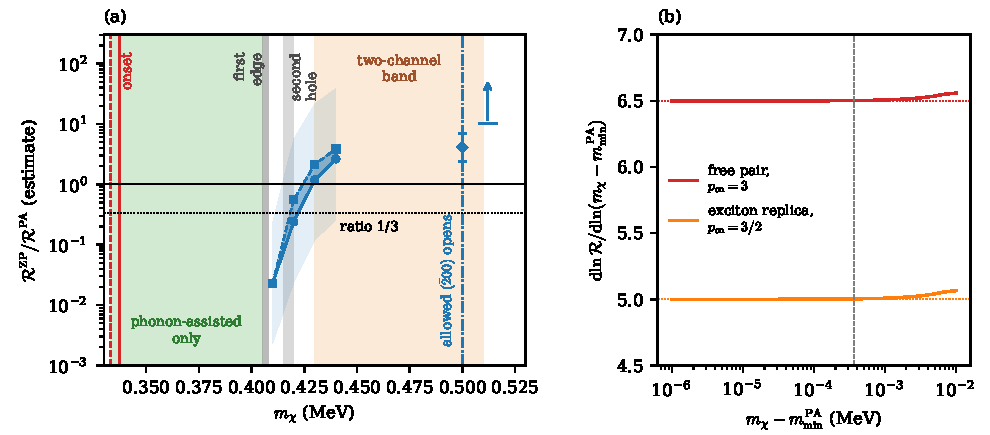
\includegraphics[width=\linewidth]{figures/ch13/fig13_9.pdf}
  \caption{Rates across the silicon window. (a)~Estimated ratio of the zero-phonon to the phonon-assisted electron-recoil rate against the dark-matter mass. Green band: phonon-assisted only, from the onsets (red: free pair \SI{0.3374}{MeV}, solid; exciton replica \SI{0.3332}{MeV}, dashed) to the first zero-phonon edge; gray bands: the first zero-phonon edge (0.405--\SI{0.408}{MeV}) and the edge of the second heavy hole (0.415--\SI{0.420}{MeV}). Blue points: the ratio with the second-hole edge at \SI{0.420}{MeV} (circles) and \SI{0.415}{MeV} (squares), each channel at the largest energy above the first edge that the mass reaches; dark band between them, light band the factor of ten of the phonon-assisted side. Diamond: the allowed $(\bar2\,0\,0)$ line at its opening, \SI{0.50}{MeV} (dash-dotted), with one or two conduction bands reached; bar and arrow: ratio of 10 or more from \SI{0.51}{MeV}. Black lines: ratio one and one third. Orange: the two-channel band. Estimates: phonon-assisted side from the measured cold absorption (\SI{20}{K} data~\cite{macfarlane1958fine}; the \SI{0.5}{K} fit of \cref{we:13-darkphoton-edge} changes the ratios by at most \SI{5}{\percent}) and a computed vertex form factor; zero-phonon side a Wannier--Mott continuum with computed vertices; between 0.44 and \SI{0.50}{MeV} no ratio has been evaluated. (b)~Local power of the model rate, $\dd\ln\mathcal{R}/\dd\ln(\mchi - m_{\mathrm{min}}^{\mathrm{PA}})$, for a loss function $Cx^{p_{\mathrm{on}}}$ above the computed transverse acoustic onset on the valley axis (PBE force constants of \cref{sec:5.2}), the standard halo (\cref{tab:1-shm}) and a heavy mediator, with the asymptotes $p_{\mathrm{on}} + 7/2$ of \cref{eq:13.9-medge} (dotted). Dashed: the mass at which the largest energy above threshold reaches \SI{1.3}{meV}, the end of the $x^3$ range of \cref{fig:13-paloss}.}
  \label{fig:13-window-rates}
\end{figure}

The phonon-assisted rate leads the electron recoil of silicon at least to about \SI{0.42}{MeV} and centrally to about \SI{0.43}{MeV}. From there to about \SI{0.51}{MeV} lies a two-channel band, in which the rates are comparable and neither can be quoted alone with confidence. Above about \SI{0.51}{MeV} the allowed zero-phonon line leads. The biases point both ways. The isotropic exciton mass underestimates the zero-phonon density of states by a factor 1.3 to 1.6, which makes the ratios too low. The form factor, more likely low than high, makes them too high; the second-hole vertex and the evaluation at the largest energy make the zero-phonon side an upper estimate. A rate computed from the amplitude on the same bins as the zero-phonon rate would settle all of it.

\subsection{Germanium and GaAs}\label{sec:13.9-ge-gaas}

The germanium window has a known lower end and an unknown upper end. Its onset, 0.2119 to \SI{0.2141}{MeV}, rests only on the gap, the position of L and the measured transverse acoustic branch (\cref{sec:13.1}); the computed PBE branch is \SI{13.5}{\percent} low at X and \SI{11.6}{\percent} low at L, so its $\omega_{\mathrm{TA}}(\vect{Q}^*) = \SI{6.70}{meV}$ on a $6^3$ grid is too soft by about as much. It places the onset at \SI{0.21380}{MeV} for a free pair and \SI{0.21264}{MeV} for the bound $1s$ exciton, with an estimated binding of \SI{4.0}{meV}. Both lie inside the bracket, and scaling the branch to the neutron data moves them by at most \SI{0.0003}{MeV}, so the softness does not reach the onset (\cref{app:E.14}). The zero-phonon edge is not known. PBE puts the conduction state at $\mathrm{\Gamma}$ below the L valley, so no scissor-corrected PBE calculation can locate it (\cref{app:E.1}), and the joint minimization on quasiparticle bands with spin--orbit coupling is open. The value \SI{0.32}{MeV} of \cref{sec:13.1}, from the parabola on the L axis, assumes a parabolic pair with the hole at $\mathrm{\Gamma}$, and it brackets the edge in neither direction. Only the joint minimum restricted to the axis, evaluated on the true bands, would be an upper value. The silicon result does not settle whether the germanium optimum leaves the axis. The [111] valley axis of germanium is already its heavy-hole direction, and the silicon optimum came from a hole moving into a flat direction away from the valley axis. What does carry over is that spin--orbit coupling must be in the bands, and that the hole must be free in the minimization. The selection rule differs as well. The mirror planes that contain a [111] axis are the diagonal planes of the $\{110\}$ family, which belong to $\bar43m$ and carry no fractional translation (\cref{app:C.17}); there is no glide phase, and on the L axis the vertex at the extrema does not vanish (\cref{sec:10.5-rules}). Whether the first zero-phonon state of germanium is weakly coupled has to be checked at its optimum. Until then germanium has a phonon-assisted onset, the onset exponent 3 for every branch (\cref{sec:13.3}), and no window.

GaAs is the control: a direct gap with its own phonon-assisted band, which in the parabolic description of the $\mathrm{\Gamma}$ pair runs from an onset of 0.433 to \SI{0.436}{MeV} to the opening of the zero-phonon channel through the L valleys, between 0.517 and \SI{0.560}{MeV} (\cref{sec:13.1}). Both ends of that bracket are rigorous for the given L energy; only the position of the edge between them needs bands. The top scales as $2E_{\mathrm{L}}/v_{\mathrm{max}}^2$, and for a detector the low-temperature L energy applies. That GaAs reproduces this band, and that its phonon-assisted rate is a small correction wherever a zero-phonon line is open, is the control that \cref{app:E.14} specifies.

\subsection{The silicon window in one table}\label{sec:13.9-table}

\Cref{tab:13-window} collects the window in two blocks: what two independent calculations or a symmetry argument with a numerical check establish, and what rests on one calculation or an estimate, or is open.

\begin{table}[tbp]
  \caption{The silicon window, with germanium and GaAs. Masses in MeV. Status: ``two independent calculations'', ``symmetry, confirmed numerically'', ``derivation'', ``one calculation'', ``measured data'', ``estimate'' (a model in which the phonon-assisted rate is known to a factor of ten either way, apart from the unsized pair channel), ``open''. Bands at the measured lattice constant with spin--orbit coupling, gap $\Eg(0) = \SI{1.170}{eV}$, halo of \cref{tab:1-shm}.}
  \label{tab:13-window}
  \centering\footnotesize\setlength{\tabcolsep}{3pt}
  \begin{tabular}{@{}>{\raggedright\arraybackslash}p{0.33\linewidth}>{\raggedright\arraybackslash}p{0.27\linewidth}>{\raggedright\arraybackslash}p{0.2\linewidth}>{\raggedright\arraybackslash}p{0.13\linewidth}@{}}
    \toprule
    Quantity & Value & Status & Section \\
    \midrule
    \multicolumn{4}{@{}l}{\emph{Established}} \\
    First zero-phonon edge, continuum & 0.405--0.408 (best 0.407); off the axis, $\{001\}$ mirror plane, tilt \SI{0.18}{rad} & two independent calculations & \cref{sec:13.9-edges} \\
    First zero-phonon edge, $1s$ line & 0.402--0.405 & two independent calculations & \cref{sec:13.9-edges} \\
    Second (mirror-even) heavy hole & from 0.415--0.420 & 0.415: two independent calculations; 0.420: estimate & \cref{sec:13.9-edges} \\
    Allowed $(\bar2\,0\,0)$ line opens & $\approx 0.50$ (X face); vertex at the class extremum $\sum_v|\rho_{cv}|^2 = 0.150$ & two independent calculations & \cref{sec:13.9-edges,sec:13.9-glide} \\
    Selection rule & first line second class by the glide; $(\bar2\,0\,0)$ class allowed; spin--orbit lift $3.6\times10^{-6}$ (axis), $1.3\times10^{-4}$ (plane) & symmetry, confirmed numerically & \cref{sec:13.9-glide} \\
    Order of the edges & onset $<$ first edge $<$ second hole $<$ allowed line & two independent calculations & \cref{sec:13.9-edges} \\
    \midrule
    \multicolumn{4}{@{}l}{\emph{Estimated or open}} \\
    Phonon-assisted onset & 0.3332 (exciton replica), 0.3374 (free pair) & one calculation & \cref{sec:13.1} \\
    Phonon-assisted rate leads & centrally to $\approx 0.43$ (0.424--0.428), at least to $\approx 0.42$ (0.418--0.421) & estimate & \cref{sec:13.9-rates} \\
    Two-channel band & 0.43--0.51 & estimate & \cref{sec:13.9-rates} \\
    Zero-phonon rate leads & above $\approx 0.51$ (ratio 2.4--7.0 at 0.50, $\ge 10$ pointwise from 0.51) & estimate & \cref{sec:13.9-rates} \\
    Screening correction relative to the optical calibration & 0.3--2.6 on $L^{\mathrm{PA}}$ (external factor and local-field wings); pair channel beyond the calibration not sized & estimate & \cref{sec:13.4,sec:13.9-rates} \\
    Rate and reach & $\sigmae \approx 3\times10^{-30}$--$3\times10^{-29}$ (0.36; the \SI{0.5}{K} fit extrapolated below \SI{1.206}{eV} carries half of it), $4\times10^{-32}\,\si{cm^2}$ (0.40), heavy mediator, \SI{1}{kg.yr}; power $p_{\mathrm{on}} + 7/2$ at the onset & estimate (factor 10 at 0.40; 15 at 0.36); power: derivation & \cref{sec:13.9-onset,sec:13.9-rates} \\
    Germanium & onset 0.2119--0.2141; zero-phonon edge not known & onset from measured data; edge open & \cref{sec:13.1,sec:13.9-ge-gaas} \\
    GaAs & phonon-assisted band 0.43 to 0.52--0.56 & estimate (parabolic $\mathrm{\Gamma}$ pair) & \cref{sec:13.1,sec:13.9-ge-gaas} \\
    \bottomrule
  \end{tabular}
\end{table}

\subsection{Nuisance table of the phonon-assisted sector}\label{sec:13.9-nuisances}

\Cref{tab:13-nuisances} collects the truncations and inputs of the chapter, each with its size and the section that treats it, in the classes of \cref{sec:8.8}.

\begin{table}[tbp]
  \caption{Nuisances of the phonon-assisted sector. Type in the classes of \cref{sec:8.8}: normalization, tilt (in $\omega$, in $q$ or in the dark-matter mass), threshold and new support. Basis of the size: ``computed'' (next order computed), ``model'' (next order computed in a model), ``est.''\ (parametric estimate), ``bound'' (only an inequality or two limits are known), ``named'' (no size). Sizes are for silicon unless another crystal is named. The last column gives the section where the item is treated.}
  \label{tab:13-nuisances}
  \centering\scriptsize\setlength{\tabcolsep}{3pt}
  \begin{tabular}{@{}>{\raggedright\arraybackslash}p{0.27\linewidth}>{\raggedright\arraybackslash}p{0.12\linewidth}>{\raggedright\arraybackslash}p{0.36\linewidth}>{\raggedright\arraybackslash}p{0.09\linewidth}>{\raggedright\arraybackslash}p{0.10\linewidth}@{}}
    \toprule
    Truncation or input & Type & Size & Basis & Section \\
    \midrule
    Transverse acoustic energy at $\vect{Q}^*$ (PBE branch \SI{8}{\percent} soft at X) & threshold & onset $+\SI{0.0004}{MeV}$ with the branch scaled to the neutron data; \SI{2.8e-4}{MeV} per meV & computed & \cref{sec:13.1} \\
    Exciton binding & threshold & phonon-assisted onset 0.3374 $\to$ \SI{0.3332}{MeV}; zero-phonon edge $-\SI{0.0028}{MeV}$ & computed & \cref{sec:13.1,sec:13.9} \\
    Fixed directions of $\vect{q}$, hole at the valence maximum & threshold & zero-phonon edge 0.405--0.408 against 0.420--\SI{0.425}{MeV} on the axis & computed & \cref{sec:13.1,sec:13.9} \\
    Spin--orbit coupling in the bands & threshold & first zero-phonon edge $+\SI{0.003}{MeV}$; on the axis $< \SI{0.0002}{MeV}$ & computed & \cref{sec:13.9} \\
    Band sum cut to empty bands & normali\-zation & $|M|^2$ off by a factor 1.6 to 2.4 in a two-band chain (two phase conventions of its phonon vertex) & model & \cref{sec:13.2} \\
    Adiabatic (Herzberg--Teller) amplitude & normali\-zation & \SI{1.6}{\percent} (TA), \SI{5.2}{\percent} (TO) at the edge; \SI{10}{\percent} when $E_{\mathrm{min}}(\vect{q}) - \omega$ falls to \SI{0.18}{eV} (TA) & est. & \cref{sec:13.2} \\
    Next order in the electron--phonon vertex ($n_g = 4$) & normali\-zation & $\theta_{\mathrm{ep}} = 0.010$--0.016 at the absorption edge; $\approx 0.2$ at the window edge & est.; bound & \cref{sec:13.3,sec:13.6} \\
    Tilt of the pair minimum, branch curvature & threshold & \SI{0.02}{meV} (TA), \SI{0.18}{meV} (LA) at \SI{1}{keV}; masses \SI{1}{\percent} & computed & \cref{sec:13.3} \\
    External screening $1/(\varepsilon_1^0)^2$ & normali\-zation & 1/30--1/38 at \SI{1}{keV}; 3.7--\SI{4.4}{\percent} across the window & computed & \cref{sec:13.4} \\
    Screening relative to the optical calibration: external model factor, local-field wings, pair channel & normali\-zation & 0.3--2.6 on $L^{\mathrm{PA}}$ for the external factor and the wings; pair ratio one in both solvable limits at exact pinning; residual from the \SI{0.2}{keV} spread of pair momenta and the range between the limits not sized & est.; named & \cref{sec:13.4,sec:13.9} \\
    Adiabatic local-density source & normali\-zation & about \SI{5}{\percent} of the pair term & est. & \cref{sec:13.4} \\
    Parabolic pockets, constant vertex (edge form) & tilt in $\omega$ & within \SI{15}{\percent} of the \SI{300}{K} data from 55 to \SI{490}{meV} above the gap; factor 2 at \SI{17}{meV} & computed & \cref{sec:13.5} \\
    Temperature of absorption data & tilt in $\omega$ & untransferred \SI{77}{K} data $\times2.3$--2.6, 1.7--1.9, 1.3--1.5, 1.1--1.3 at 15, 25, 50, \SI{100}{meV}; strength factor 0.88 (\SI{77}{K}), 0.61 (\SI{295}{K}); branch weights $\pm\SI{25}{\percent}$: $<\SI{1}{\percent}$ from \SI{77}{K} & computed & \cref{sec:13.5} \\
    Cold absorption data: \SI{0.5}{K} fit against \SI{20}{K} data & normali\-zation; tilt in $\omega$ & $\times20$ at \SI{1.20}{eV}, $\times2.1$ at \SI{1.25}{eV}, within \SI{5}{\percent} above \SI{1.37}{eV}; rate $\times9$ at \SI{0.36}{MeV}, $\times1.8$ at \SI{0.40}{MeV}; \SI{55}{\percent} of the \SI{0.36}{MeV} rate from the fit below its lowest data point & computed & \cref{sec:13.8,sec:13.9} \\
    Margin of the off-shell window, pair widths & tilt in $q$ & controlling ratios $\le 0.21$ at $\delta_{\mathrm{w}} = \SI{0.3}{eV}$; widths 3--\SI{21}{meV}; window to $|\vect{q}| = \SI{1.33}{keV}$ (parabolic), \SI{1.27}{keV} (computed bands) & est.; model & \cref{sec:13.6} \\
    Fano term & tilt & zero in Si and Ge; GaAs $\lesssim 0.3\varGamma/\delta_{\mathrm{F}}$, a few percent of first emissions moved & est. & \cref{sec:13.6} \\
    Nonadiabatic zero-point renormalization & threshold & \SI{8}{meV} on the gap; onset \SI{0.0023}{MeV} if the gap is built from a computed renormalization; with the measured gap only its variation across the zone, zero-phonon edge $\le\SI{0.002}{MeV}$ & computed; bound & \cref{sec:13.7} \\
    Exciton--phonon replicas beyond the two-pair sector & new support & no size & named & \cref{sec:13.8} \\
    Singlet against triplet pairs in axion-like absorption & normali\-zation & no pair channel in the triplet response, size not known; replica lines shifted by the exchange splitting, about $2\times10^{-3}$ of $E_x^b$ & named (open) & \cref{sec:13.8} \\
    Finite-$q$ form factor of the rate estimate & normali\-zation; tilt in $\mchi$ & factor 3; combined factor 6.5 at 0.38--\SI{0.43}{MeV}, quoted as 10 & est. & \cref{sec:13.9} \\
    Completeness of the plane-wave band sum ($f$-sum) & normali\-zation & 0.81 $\to$ 0.89 of $q^2/2m_e$ with 16 $\to$ 100 bands; nonlocal and truncation parts not separated & computed & \cref{sec:13.9} \\
    Zero-phonon side of the ratio (isotropic exciton mass, second-hole vertex) & normali\-zation & density of states low by 1.3--1.6; second-hole term an upper estimate & est. & \cref{sec:13.9} \\
    Spin--orbit lift of symmetry zeros & new support & zero-phonon ratio $\le 0.01$; longitudinal acoustic kink $<10^{-4}$ on the axis & computed; est. & \cref{sec:13.3,sec:13.9} \\
    \bottomrule
  \end{tabular}
\end{table}

For the rate in the window, three rows dominate: the finite-$q$ form factor of the estimate, a factor three either way and probably low; the screening correction relative to the optical calibration, whose pair-channel part no calculation sizes; and, near the onset, the spread of the cold data. Every threshold row is small in mass, a few thousandths of an MeV at most, and the order of the edges survives all of them together. What a threshold error costs, however, is not small near the onset, where \cref{eq:13.9-medge} raises it to the power $p_{\mathrm{on}} + 7/2$.

\subsection{Open problems}\label{sec:13.9-open}

The onset rests on one set of force constants, soft on exactly the branch that sets it, and a direct calculation of $\omega_{\mathrm{TA}}(\vect{Q}^*)$ at two lattice constants and with a second pseudopotential would verify it (\cref{app:E.14}). The end of the phonon-assisted lead, the width of the two-channel band and the mass from which the zero-phonon line leads follow from the ratio of the two rates computed on common bins, with the full amplitude on the phonon-assisted side and the mirror-plane cones, the second heavy hole and the X-face edge on the zero-phonon side (\cref{app:E.14}). The same calculation gives the rate and the reach with their controls: the optical limit, the symmetry zeros, the soft acoustic limit and the completeness of the band sum, whose plane-wave $f$-sum with a norm-conserving pseudopotential reaches 0.81 of $q^2/2m_e$ with 16 bands and 0.89 with 100 at $|\vect{q}| = 0.1$ to \SI{0.5}{\angstrom^{-1}}, the bands left out and the nonlocal term not yet separated. The pair channel beyond the optical calibration needs the supercell calculation of \cref{app:E.16}, with local fields in the supercell basis. Germanium needs quasiparticle bands with spin--orbit coupling for its zero-phonon edge and phonons that pass the neutron data on the transverse acoustic branch, and GaAs, the control of the whole chain, its band calculation and its rate with the polar vertex (\cref{app:E.14}).

One measurement would test the chain directly: the cold absorption edge of silicon within \SI{25}{meV} of its threshold, which no measurement at millikelvin temperatures covers. There the untransferred \SI{77}{K} data are off by more than a factor of two (\cref{sec:13.5}), and the two cold datasets of \cref{sec:13.9-rates} differ by a factor of twenty at \SI{1.20}{eV}.

\section*{Summary}

Dark matter lighter than about \SI{0.4}{MeV} cannot create an electron--hole pair in silicon on its own: where it deposits the gap it transfers about \SI{0.9}{keV}, and a pair with that momentum costs more than the gap. A phonon of about \SI{15}{meV} takes the missing crystal momentum (\cref{sec:13.1}). The lightest mass that creates a pair without a phonon is a joint minimum over the momentum transfer and the hole's crystal momentum. The lightest that creates one with a phonon is the kinematic floor with the gap raised by one phonon energy, at the wavevector the dark matter leaves for the phonon: \SI{0.3374}{MeV} for the free pair, \SI{0.3332}{MeV} for the exciton replica. The onset is insensitive to the band structure and rests on one phonon energy. Germanium has its onset at 0.212 to \SI{0.214}{MeV} from the measured transverse acoustic branch alone, and GaAs, though direct, has a phonon-assisted band of its own above \SI{0.433}{MeV}, because its light pair cannot absorb the momentum either.

The amplitude is of second order, one density vertex and one electron--phonon vertex on four paths (\cref{sec:13.2}). The exclusion principle turns the paths through filled states into exchange partners of the blocked ones, and on shell the amplitude becomes a one-electron sum over all bands, filled ones included; cutting it to empty bands is wrong by a factor of order one. The intraband terms cancel at $\vect{q} = 0$, so the amplitude starts at first order in $q$. It does not interfere with the zero-phonon line, whose final states have one phonon fewer. Its adiabatic form is the derivative of the zero-phonon transition density with respect to a frozen phonon, the Herzberg--Teller term, accurate to a few percent at the absorption edge.

Squared and summed, the amplitude gives the phonon-assisted structure factor and loss function, which enter the rate exactly as the zero-phonon ones do (\cref{sec:13.3}). Inside the off-shell window they are the whole electronic response; above the zero-phonon edge they add to it, and the $f$-sum rule they share forbids adding a bare zero-phonon rate to them without the renormalization of \cref{sec:13.7}. At its threshold the direction-averaged loss function rises as the cube of the energy above it, as the fourth power at the longitudinal acoustic kink, which a selection rule on the valley axis forbids, and as the power 3/2 for an exciton replica.

Screening acts on the density vertex and on the final pair (\cref{sec:13.4}). The external factor is one inverse macroscopic dielectric function for the whole amplitude, $1/30$ to $1/38$ in the loss function at \SI{1}{keV} in silicon, far from the optical $1/\varepsilon_\infty^2$. The pair channel screens at the pinned momentum of the final pair, the same for every $\vect{q}$; its size and sign are open, bracketed only by two solvable limits a factor of ten apart, and in both limits a measured optical edge calibrates it at every $\vect{q}$.

As $\vect{q} \to 0$ the loss function becomes phonon-assisted optical absorption, by the continuity equation applied to the second-order amplitude (\cref{sec:13.5}). The measured edge of silicon is its test: the Hall--Bardeen--Blatt form, with one fitted scale, lies within \SI{15}{\percent} of the \SI{300}{K} data over 55 to \SI{490}{meV} above the gap. Absorption data must be transferred to the temperature of a detector branch by branch. The inverse transfer is exact for branch-resolved spectra and ill-posed without them, and untransferred \SI{77}{K} data overstate the cold edge by more than a factor of two within 18 to \SI{23}{meV} of it.

Two kinds of small denominator threaten the amplitude (\cref{sec:13.6}). Soft acoustic phonons give finite amplitudes once the recoil, deformation and velocity terms of a Ward identity are kept, and inside the window the soft limit is never reached. Zero-phonon detunings fix the window. The phonon-assisted rate is a channel of its own only where every first-order transition is off shell by a margin, \SI{0.3}{eV} in silicon. The margin confines it to $|\vect{q}| \le \SI{1.33}{keV}$ on the valley axis in the parabolic description and \SI{1.27}{keV} with the computed bands. Beyond the window only totals are defined, with the Dyson convention, and the Fano term vanishes in silicon and germanium.

At finite temperature and zero point the bands are renormalized, and a special-displacement calculation contains the adiabatic sideband, which places the phonon-assisted onset one phonon energy too low (\cref{sec:13.7}). Between room temperature and \SI{10}{mK} the gap opens by \SI{46}{meV} and the onset moves from 0.324 to \SI{0.337}{MeV}; below a few kelvin the window does not move. The nonadiabatic part of the zero-point renormalization, \SI{8}{meV} on the silicon gap, is already in the measured gap, and only its variation across the zone, at most \SI{0.002}{MeV} on the zero-phonon edge, can move the window. Excitons with phonons add replica edges below the free-pair edges, each rising as a square root at fixed $\vect{q}$, with a completeness condition that reduces to the two-pair sector; at the optical edge of cold silicon they carry most of the absorption. The same vertices give the phonon-assisted absorption of dark photons, axion-like particles and scalars at the indirect edge; the dark photon has no new pair-plus-phonon amplitude at first order in its coupling (\cref{sec:13.8}).

In silicon the first zero-phonon edge lies at 0.405 to \SI{0.408}{MeV}, off the valley axis in a mirror plane, with its $1s$ line at 0.402 to \SI{0.405}{MeV} (\cref{sec:13.9}). The glide of the diamond structure forbids its vertex, so the first zero-phonon line is weak; the second heavy hole opens from 0.415 to \SI{0.420}{MeV}, and an allowed Umklapp line of full size opens at \SI{0.50}{MeV}, where the same glide inverts the rule. These edges, the rule and their order are established. Between the onset and the first edge the phonon-assisted rate is the only electron-recoil channel. Its rate rises from the onset as the power $p_{\mathrm{on}} + 7/2$ of the distance in mass, so that near the onset only the exponent is predicted. By an estimate normalized to the measured cold edge, with rates uncertain by a factor of ten apart from the pair channel's dependence on $q$, it leads to about \SI{0.43}{MeV}, the two channels share 0.43 to \SI{0.51}{MeV}, and the zero-phonon line leads above. The nuisances of the chapter are collected in \cref{tab:13-nuisances}. Germanium and GaAs need quasiparticle band calculations. Throughout, the dark matter coupled to the electron density, which does not act on spin; \cref{chap:14} turns to couplings that reach the spins of a magnet.

\printbibliography[heading=subbibliography]
